% Options for packages loaded elsewhere
\PassOptionsToPackage{unicode}{hyperref}
\PassOptionsToPackage{hyphens}{url}
\documentclass[
]{book}
\usepackage{xcolor}
\usepackage{amsmath,amssymb}
\setcounter{secnumdepth}{5}
\usepackage{iftex}
\ifPDFTeX
  \usepackage[T1]{fontenc}
  \usepackage[utf8]{inputenc}
  \usepackage{textcomp} % provide euro and other symbols
\else % if luatex or xetex
  \usepackage{unicode-math} % this also loads fontspec
  \defaultfontfeatures{Scale=MatchLowercase}
  \defaultfontfeatures[\rmfamily]{Ligatures=TeX,Scale=1}
\fi
\usepackage{lmodern}
\ifPDFTeX\else
  % xetex/luatex font selection
\fi
% Use upquote if available, for straight quotes in verbatim environments
\IfFileExists{upquote.sty}{\usepackage{upquote}}{}
\IfFileExists{microtype.sty}{% use microtype if available
  \usepackage[]{microtype}
  \UseMicrotypeSet[protrusion]{basicmath} % disable protrusion for tt fonts
}{}
\makeatletter
\@ifundefined{KOMAClassName}{% if non-KOMA class
  \IfFileExists{parskip.sty}{%
    \usepackage{parskip}
  }{% else
    \setlength{\parindent}{0pt}
    \setlength{\parskip}{6pt plus 2pt minus 1pt}}
}{% if KOMA class
  \KOMAoptions{parskip=half}}
\makeatother
\usepackage{color}
\usepackage{fancyvrb}
\newcommand{\VerbBar}{|}
\newcommand{\VERB}{\Verb[commandchars=\\\{\}]}
\DefineVerbatimEnvironment{Highlighting}{Verbatim}{commandchars=\\\{\}}
% Add ',fontsize=\small' for more characters per line
\usepackage{framed}
\definecolor{shadecolor}{RGB}{248,248,248}
\newenvironment{Shaded}{\begin{snugshade}}{\end{snugshade}}
\newcommand{\AlertTok}[1]{\textcolor[rgb]{0.94,0.16,0.16}{#1}}
\newcommand{\AnnotationTok}[1]{\textcolor[rgb]{0.56,0.35,0.01}{\textbf{\textit{#1}}}}
\newcommand{\AttributeTok}[1]{\textcolor[rgb]{0.13,0.29,0.53}{#1}}
\newcommand{\BaseNTok}[1]{\textcolor[rgb]{0.00,0.00,0.81}{#1}}
\newcommand{\BuiltInTok}[1]{#1}
\newcommand{\CharTok}[1]{\textcolor[rgb]{0.31,0.60,0.02}{#1}}
\newcommand{\CommentTok}[1]{\textcolor[rgb]{0.56,0.35,0.01}{\textit{#1}}}
\newcommand{\CommentVarTok}[1]{\textcolor[rgb]{0.56,0.35,0.01}{\textbf{\textit{#1}}}}
\newcommand{\ConstantTok}[1]{\textcolor[rgb]{0.56,0.35,0.01}{#1}}
\newcommand{\ControlFlowTok}[1]{\textcolor[rgb]{0.13,0.29,0.53}{\textbf{#1}}}
\newcommand{\DataTypeTok}[1]{\textcolor[rgb]{0.13,0.29,0.53}{#1}}
\newcommand{\DecValTok}[1]{\textcolor[rgb]{0.00,0.00,0.81}{#1}}
\newcommand{\DocumentationTok}[1]{\textcolor[rgb]{0.56,0.35,0.01}{\textbf{\textit{#1}}}}
\newcommand{\ErrorTok}[1]{\textcolor[rgb]{0.64,0.00,0.00}{\textbf{#1}}}
\newcommand{\ExtensionTok}[1]{#1}
\newcommand{\FloatTok}[1]{\textcolor[rgb]{0.00,0.00,0.81}{#1}}
\newcommand{\FunctionTok}[1]{\textcolor[rgb]{0.13,0.29,0.53}{\textbf{#1}}}
\newcommand{\ImportTok}[1]{#1}
\newcommand{\InformationTok}[1]{\textcolor[rgb]{0.56,0.35,0.01}{\textbf{\textit{#1}}}}
\newcommand{\KeywordTok}[1]{\textcolor[rgb]{0.13,0.29,0.53}{\textbf{#1}}}
\newcommand{\NormalTok}[1]{#1}
\newcommand{\OperatorTok}[1]{\textcolor[rgb]{0.81,0.36,0.00}{\textbf{#1}}}
\newcommand{\OtherTok}[1]{\textcolor[rgb]{0.56,0.35,0.01}{#1}}
\newcommand{\PreprocessorTok}[1]{\textcolor[rgb]{0.56,0.35,0.01}{\textit{#1}}}
\newcommand{\RegionMarkerTok}[1]{#1}
\newcommand{\SpecialCharTok}[1]{\textcolor[rgb]{0.81,0.36,0.00}{\textbf{#1}}}
\newcommand{\SpecialStringTok}[1]{\textcolor[rgb]{0.31,0.60,0.02}{#1}}
\newcommand{\StringTok}[1]{\textcolor[rgb]{0.31,0.60,0.02}{#1}}
\newcommand{\VariableTok}[1]{\textcolor[rgb]{0.00,0.00,0.00}{#1}}
\newcommand{\VerbatimStringTok}[1]{\textcolor[rgb]{0.31,0.60,0.02}{#1}}
\newcommand{\WarningTok}[1]{\textcolor[rgb]{0.56,0.35,0.01}{\textbf{\textit{#1}}}}
\usepackage{longtable,booktabs,array}
\usepackage{calc} % for calculating minipage widths
% Correct order of tables after \paragraph or \subparagraph
\usepackage{etoolbox}
\makeatletter
\patchcmd\longtable{\par}{\if@noskipsec\mbox{}\fi\par}{}{}
\makeatother
% Allow footnotes in longtable head/foot
\IfFileExists{footnotehyper.sty}{\usepackage{footnotehyper}}{\usepackage{footnote}}
\makesavenoteenv{longtable}
\usepackage{graphicx}
\makeatletter
\newsavebox\pandoc@box
\newcommand*\pandocbounded[1]{% scales image to fit in text height/width
  \sbox\pandoc@box{#1}%
  \Gscale@div\@tempa{\textheight}{\dimexpr\ht\pandoc@box+\dp\pandoc@box\relax}%
  \Gscale@div\@tempb{\linewidth}{\wd\pandoc@box}%
  \ifdim\@tempb\p@<\@tempa\p@\let\@tempa\@tempb\fi% select the smaller of both
  \ifdim\@tempa\p@<\p@\scalebox{\@tempa}{\usebox\pandoc@box}%
  \else\usebox{\pandoc@box}%
  \fi%
}
% Set default figure placement to htbp
\def\fps@figure{htbp}
\makeatother
\setlength{\emergencystretch}{3em} % prevent overfull lines
\providecommand{\tightlist}{%
  \setlength{\itemsep}{0pt}\setlength{\parskip}{0pt}}
\usepackage[]{natbib}
\bibliographystyle{apalike}
\usepackage{booktabs}
\usepackage{amsthm}
\makeatletter
\def\thm@space@setup{%
  \thm@preskip=8pt plus 2pt minus 4pt
  \thm@postskip=\thm@preskip
}
\makeatother
\usepackage{bookmark}
\IfFileExists{xurl.sty}{\usepackage{xurl}}{} % add URL line breaks if available
\urlstyle{same}
\hypersetup{
  pdftitle={Quantitive Methods 2, ZHAW},
  pdfauthor={Jürgen Degenfellner},
  hidelinks,
  pdfcreator={LaTeX via pandoc}}

\title{Quantitive Methods 2, ZHAW}
\author{Jürgen Degenfellner}
\date{2025-02-07}

\begin{document}
\maketitle

{
\setcounter{tocdepth}{1}
\tableofcontents
}
\chapter{Introduction}\label{intro0}

This script is a continuation of
\href{https://jdegenfellner.github.io/Script_QM1_ZHAW/}{the first one} for Quantitative Methods 1
at ZHAW.

In the first part, we learned about the basics of probability theory,
descriptive statistics, Bayesian statistics, and hypothesis testing.

In this script, we will dive into the basics of statistical modeling -
a world of aesthetic wonder and surprises.

This script is a first draft as you are the first group to be working with it.

Please feel free to send me suggestions for improvements or corrections.

This \textbf{should be a collaborative effort} and will (hopefully)
never be finished as our insight grows over time.

The script can also be seen as a pointer to great sources which are
fit to deepen your understanding of the topics. Knowledge is decentralized,
and there are many great ressources out there.

For the working setup with R, please
see \href{https://jdegenfellner.github.io/Script_QM1_ZHAW/index.html\#section}{this}
and the following sections in the first script.

The complete code for this script can be found
\href{https://github.com/jdegenfellner/Script_QM2_ZHAW}{here}.

\section{Books we will heavily borrow from are:}\label{books-we-will-heavily-borrow-from-are}

\begin{itemize}
\tightlist
\item
  (Free) \href{https://civil.colorado.edu/~balajir/CVEN6833/bayes-resources/RM-StatRethink-Bayes.pdf}{Statistical Rethinking}, YouTube-Playlist: \href{https://youtu.be/FdnMWdICdRs?si=q2py5QVY_L299hEa}{Statistical Rethinking 2023}
\item
  (Free) \href{https://vdoc.pub/documents/understanding-regression-analysis-a-conditional-distribution-approach-84oqjr8sqva0}{Understanding Regression Analysis: A Conditional Distribution Approach}
\item
  \href{http://www.stat.columbia.edu/~gelman/arm/}{Data Analysis Using Regression and Multilevel/Hierarchical Models}
\item
  (Free) \href{https://nyu-cdsc.github.io/learningr/assets/kruschke_bayesian_in_R.pdf}{Doing Bayesian Data Analysis}
\end{itemize}

\section{If you need a good reason to buy good books\ldots{}}\label{if-you-need-a-good-reason-to-buy-good-books}

Think of the total costs of your education. You want to extract maximum
benefit from it. In the US, an education costs \href{https://www.finaid.ucsb.edu/docs/default-source/default-document-library/2024-2025-undergrad-coa.pdf?sfvrsn=fb791f8a_4}{a lot}.
In beautiful Switzerland, the \href{https://www.zhaw.ch/de/sml/studium/master/kosten}{tuition fees} (if applicable) are nowhere near these figures.
Costs you could consider are opportunity costs of not working.
A comparison with both, a foreign education or opportunity costs,
justifies the investment in good books.
Or: The costs of all the good books of your education combined are probably less than an iPhone Pro.

\chapter{Introduction}\label{intro}

\section{What is statistical modeling and what do we need this for?}\label{what-is-statistical-modeling-and-what-do-we-need-this-for}

Typically, one simplifies the complex reality (and loses information) in order to make it better
understandable, mathematically treatable and to make predictions.

Underlying our models, there are theories which should be \href{https://en.wikipedia.org/wiki/Falsifiability}{falsifiable}
and testable.
For instance, I would be really surprised if I pull up my multimeter and measure the voltage (V) and
electric current (I) at a resistence (R) in a circuit and find that \href{https://en.wikipedia.org/wiki/Ohm\%27s_law}{Ohm's law} \(V = IR\) is not true.
This \href{https://en.wikipedia.org/wiki/Scientific_law}{\textbf{law}}
can be tested over and over again and if one would find a single valid counterexample,
the law would be falsified. It is also true that the law is probably not 100\% accularate,
but an extremely good approximation of reality. Real-world measurements carry
measurement errors and when plotting the data, one would see that the data points
might not lie exactly on a straight line. This is not a problem.

A \href{https://en.wikipedia.org/wiki/Statistical_model}{statistical model}
is a mathematical framework that represents the
relationships between variables, helping us understand, infer, and
predict patterns in data. It acts as a bridge between observed data
and the real-world processes that generated them. In health research,
where variability and uncertainty are inherent, statistical models are
valuable tools for making sense of complex phenomena.
You can watch \href{https://www.youtube.com/watch?v=3d5ivs_8amQ&ab_channel=VeryNormal}{this} as short intro.

In \href{https://jdegenfellner.github.io/Script_QM1_ZHAW/probs.html}{QM1} we have already
made testable predictions with respect to the probability of an event.
In our 1000-researcher experiment we stated for instance, that the probability of
obeserving \(66\) or more findings would be very unlikely. If such an event would
occur (while not repeating the experiment many times), we would reconsider our model.
Inexactly, we could have stated something like: ``We will not see more than 100 findings by chance.''
With respect to our multiple choice test we could predict:
``We will not see a single person answering all questions correctly by chance in our
lifetime (given the frequency of tests).'' Note, that in this context, the word \textbf{predict}
is used with respect to a future event (chance finding or chance passing of the test).
As we will see, there does not necessarily have to be a temporal connection in order
to \emph{predict} something.

Depending on the task at hand, we would use different models.
In any case, logical reasoning and critical thinking comes first,
then comes the model. \textbf{It makes no sense to estimate statistical models just for the sake of it}.

\textbf{All models are wrong, but some are useful}.
Or to quote \href{https://www.tandfonline.com/doi/abs/10.1080/01621459.1976.10480949}{George Box}:

\begin{quote}
``Since all models are wrong the scientist cannot obtain
a `correct' one by excessive elaboration. On the contrary
following William of Occam he should seek an economical
description of natural phenomena. Just as the ability to
devise simple but evocative models is the signature of the
great scientist so overelaboration and overparameterization is often the mark of mediocrity.''
\end{quote}

In my opinion, statistical modeling is an art form: difficult and beautiful.

\textbf{One goal of this course} is to improve interpretation and limitations of statistical models.
They are not magical turning data into truth. Firstly, the rule gargabe in, garbage out (GABA) applies.
Secondly, statistical models are based on data and their variability and have inherent limitations
one cannot overcome even with the most sophisticated models. This is expressed for instance
in the so-called \href{https://en.wikipedia.org/wiki/Bias\%E2\%80\%93variance_tradeoff}{bias-variance trade-off}.
You can't have it all.

\subsection{Explanatory vs.~Predictive Models}\label{explanatory-vs.-predictive-models}

I can recommend reading \href{https://projecteuclid.org/journals/statistical-science/volume-25/issue-3/To-Explain-or-to-Predict/10.1214/10-STS330.full}{this}
article by Shmueli et al.~(2010) on this topic.

Statistical models serve different purposes depending on the research question. Two primary goals are \textbf{explanation}
and \textbf{prediction}, and each requires a different approach:

\textbf{Explanatory Models} focus on understanding causal relationships.
These models aim to uncover mechanisms and answer \textbf{``why''}
questions. For example:

\begin{itemize}
\tightlist
\item
  Does smoking increase the risk of lung cancer? \textbf{Yes}. (If you want to see what a large effect-size looks like, check out \href{https://bmjopen.bmj.com/content/bmjopen/8/10/e021611.full.pdf}{this study}.)
\item
  How large is the \textbf{effect} (causal) of smoking on lung cancer? \textbf{Large}.
\item
  Does pain education and graded sensorimotor relearning improve disability (a question we ask in
  our \href{https://data.snf.ch/grants/grant/220585}{Resolve Swiss project})?
\end{itemize}

Explanatory models are \textbf{theory-driven}, designed to test hypotheses. Here, one wants to understand the underlying
mechanisms and the relationships between variables and hence often uses (parsimonious) models that are more interpretable,
like linear regression.

\textbf{Predictive Models} prioritize forecasting future outcomes based on patterns in the data.
These models aim to answer \textbf{``what will happen?''} For instance:

\begin{itemize}
\tightlist
\item
  \href{https://www.tandfonline.com/doi/abs/10.1080/03091902.2020.1822940}{Gait analysis} using Machine Learning (ML)?
\item
  \href{https://jamanetwork.com/journals/jamadermatology/fullarticle/2756346}{Skin cancer detection} using neural networks?
\end{itemize}

Predictive models are \textbf{data-driven}, often using complex algorithms to achieve high accuracy.
Their success is measured using metrics like \href{https://computersciencewiki.org/index.php/Root-mean-square_error_(RMSE)}{Root Means Square Error}
(RMSE), \href{https://en.wikipedia.org/wiki/Receiver_operating_characteristic\#:~:text=The\%20area\%20under\%20the\%20curve,ranks\%20higher\%20than\%20'negative'}{Area Unter the Curve}
(AUC), or \textbf{prediction error on new, unseen data}.
Any amount of model complexity is allowed. One could for instance estimate a
\href{https://en.wikipedia.org/wiki/Neural_network_(machine_learning)}{neural network} (``just'' another statistical model)
with many hidden layers and neurons in order to improve prediction quality. Interpretability of the model weights is not a priority here.

While explanatory and predictive goals often complement each other,
their differences highlight the importance of clearly defining the purpose
of your analysis. In applied health research, explanatory models help identify
causal mechanisms, while predictive models can guide real-world decisions by
providing actionable forecasts. Together, they enhance both our understanding
of phenomena and our ability to make informed decisions in complex environments.

\subsection{Individual vs.~Population Prediction}\label{individual-vs.-population-prediction}

Another important distinction is between \textbf{individual vs.~population} prediction.
In the smoking example above, we can be very sure about the mean effects that smoking has on lung cancer.
On an individual level, it is \href{https://www.liebertpub.com/doi/10.1089/rej.2019.2298}{harder to predict the outcome}.
Nevertheless, individual predictions will be (notably) better than random guessing. We will discuss this in greater detail.

\subsection{Practical Use of Statistical Models}\label{practical-use-of-statistical-models}

In my optinion, we should never be afraid to test our statistical models (as honestly as possible) against reality.
We could for instance ask ourselves:

\begin{itemize}
\item
  ``How much better does this model classify than the arithmetic mean?
  (i.e., the linear model with just an intercept)''
\item
  ``How much better does this model classify than random guessing?''
\item
  Is it worth the effort to collect data and estimate this model by using hundreds of hours of our time?
\end{itemize}

In some cases, these questions can be answered straightforwardly.

\begin{itemize}
\item
  In advertising (Google, Facebook, \ldots), a couple of percentage points in prediction quality might make a difference of millions
  of dollars in revenue offsetting the statistitians salary.
\item
  Improved forecasts of a few percentage points in the stock market or just being \href{https://en.wikipedia.org/wiki/Jim_Simons}{slightly better}
  than the average, will make you faboulously rich.
\item
  Improved cancer forecasting might save lives, money and pain and is not only measured in money.
\end{itemize}

\subsection{Start at the beginning}\label{start-at-the-beginning}

What do we actually want to do in general? Very broadly speaking we want to:
\textbf{describe} the association of variables to each other that carry variability.
Hence, the relationship is not deterministic like \[y = 2x + 3\] but rather we need
to ``loosen up'' the relationship to account for variability (in \(x\) and \(y\)).
So, \(y\) and \(x\) are not fixed but aflicted with uncertainty.
Depending on your philosophical view, you might say you want to find
the ``true'' but unknown relationship (here, \(2\) and \(3\) are the true coefficients) between variables.
This is what we do in simulation studies all the time: We know the true relationship,
simulate data by adding variability and then try to estimate the true relationship we assumed in the first place.
This is an \textbf{advantage} the pioneers of statistics did not have. We can simulate
millions of lines of data at the click of a button.
For some practical applications, we can get a really nice and complete answer to our question
(for instance sample size for proportions).

So we are looking for a function \(f\) such that

\[ Y = f(X) \]

where

\begin{itemize}
\tightlist
\item
  \(Y\) is the ``outcome'', ``dependent variable'' or ``response''.
\item
  \(X\) are the ``predictors''. \(X\) can be a single Variable \(x\) or many
  variables \(x_1, x_2, \ldots, x_p\).
\end{itemize}

It is important to be aware of the notation here:
``Predict'' does \textbf{not necessarily} mean that we can predict the value in
the future. It merely means we estimate the value (or mean) of \(Y\) given \(X\).

\begin{itemize}
\tightlist
\item
  This can be done at the same time points, known as \textbf{cross-sectional} analysis (``What is the maximum jumping height
  of a person given their age at a certain point in time, whereas both variables are measured at the same time?'');
\item
  or at different time points, known as \textbf{longitudinal analysis} (``What is the maximum jumping height of a person 10 years later (\(t_2\))
  given their baseline health status at time \(t_1\)?'').
\end{itemize}

The \textbf{simplest statistical model} would be the mean model where \(Y\) is ``predicted'' by a
constant: \(Y = c\) which (at least in the classical linear regression) turns out to be \(c = \bar{x}\).
This simple model is often surprisingly good, or, to put it in other words, models with more complexity
are often not that much better.

\section{A (simple) model for adult body heights in the Bayesian framework}\label{a-simple-model-for-adult-body-heights-in-the-bayesian-framework}

As repetition, read the parts about \href{https://jdegenfellner.github.io/Script_QM1_ZHAW/bayes_statistics.html}{Bayes statistics from QM1}
again to refresh your memory about the Bayesian framework.

It's recommendable to read the beginning of the book \href{https://civil.colorado.edu/~balajir/CVEN6833/bayes-resources/RM-StatRethink-Bayes.pdf}{Statistical rethinking}
(hint: the online-version of the book differs a bit from the paper-version)
up until page 39 as well. We are not completely new to the topic of Bayes due
to QM1.

We want to \textbf{start building our first model} right away.

Let's begin with the example in
\href{https://civil.colorado.edu/~balajir/CVEN6833/bayes-resources/RM-StatRethink-Bayes.pdf}{Statistical rethinking}
using data from the \href{https://en.wikipedia.org/wiki/\%C7\%83Kung_people}{!Kung San}
people.

\begin{Shaded}
\begin{Highlighting}[]
\FunctionTok{library}\NormalTok{(rethinking)}
\FunctionTok{data}\NormalTok{(}\StringTok{"Howell1"}\NormalTok{)}
\NormalTok{d }\OtherTok{\textless{}{-}}\NormalTok{ Howell1}
\FunctionTok{str}\NormalTok{(d)}
\end{Highlighting}
\end{Shaded}

\begin{verbatim}
## 'data.frame':    544 obs. of  4 variables:
##  $ height: num  152 140 137 157 145 ...
##  $ weight: num  47.8 36.5 31.9 53 41.3 ...
##  $ age   : num  63 63 65 41 51 35 32 27 19 54 ...
##  $ male  : int  1 0 0 1 0 1 0 1 0 1 ...
\end{verbatim}

\begin{Shaded}
\begin{Highlighting}[]
\NormalTok{d2 }\OtherTok{\textless{}{-}}\NormalTok{ d[d}\SpecialCharTok{$}\NormalTok{age }\SpecialCharTok{\textgreater{}=} \DecValTok{18}\NormalTok{, ] }\CommentTok{\# only adults}
\end{Highlighting}
\end{Shaded}

We want to model the adult height of the !Kun San people
using prior knowledge (about the Swiss population) and data.

\begin{Shaded}
\begin{Highlighting}[]
\FunctionTok{library}\NormalTok{(tidyverse)}
\NormalTok{d2 }\SpecialCharTok{\%\textgreater{}\%} \FunctionTok{ggplot}\NormalTok{(}\FunctionTok{aes}\NormalTok{(}\AttributeTok{x =}\NormalTok{ height)) }\SpecialCharTok{+} \FunctionTok{geom\_histogram}\NormalTok{()}
\end{Highlighting}
\end{Shaded}

\pandocbounded{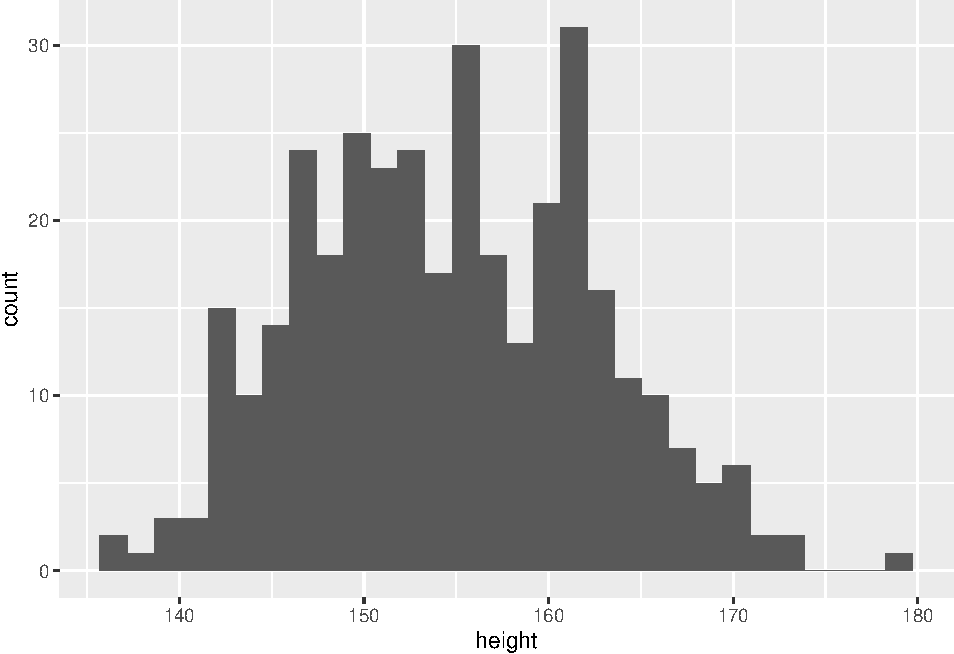
\includegraphics[keepaspectratio]{bookdown-demo_files/figure-latex/unnamed-chunk-2-1.pdf}}

Since we already have domain knowledge in this area, we can say that heights are usually normally distributed,
or at least a mixture of normal distrubutions (female/male).
We assume the following model:
\[h_i \sim \text{Normal}(\mu, \sigma)\]

As in \href{https://jdegenfellner.github.io/Script_QM1_ZHAW/}{QM1},
we want to start with a Bayesian model and hence, we need some priors.

Since we are in Switzerland and just for fun, we use the mean of
\href{https://www.bfs.admin.ch/asset/de/30305714}{Swiss body heights}
as expected value for the \textbf{prior for the mean}.
According to the link (Bundesamt für Statistik),
the mean height of \(n=21,873\) people in the Swiss sample is
\(171.1\) cm. We choose the same \(\sigma\) for the prior of the normal
as in the book not to deviate too much from the example at hand.

Next comes our \textbf{model definition in the Bayesian framework}, which
I often find more intuitive than the frequentist approach:

\[
h_i \sim \text{Normal}(\mu, \sigma)
\]
\[
\mu \sim \text{Normal}(171.1, 20)
\]
\[
\sigma \sim \text{Uniform}(0, 50)
\]

\textbf{Description of the model definition}: The heights are normally distributed with unknown mean and
standard deviation. As our current knowledge about the mean height, we use
a prior distribution for the mean (we do not know but want to estimate) by
assuming the mean of a population we know and a standard deviation of \(20\) cm which
allows are rather large range of possible values for \(\mu\)
(the unobserved population mean of the !Kung San people).
\(\sigma\) (the unobserved standard deviation of the population of !Kun San people)
is also unknown and a priori we restrict ourselves to values
between \(0\) and \(50\) cm, whereas we assign equal plausibility to all
values in this range (which can and should be critically discussed).

\textbf{Vizualisation of the model structure}:
\pandocbounded{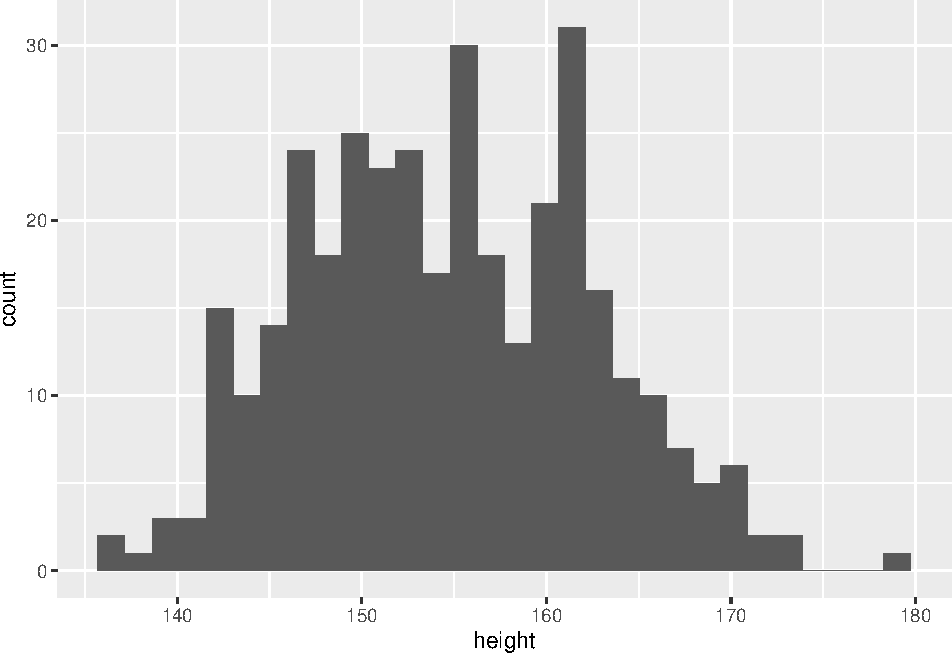
\includegraphics[keepaspectratio]{bookdown-demo_files/figure-latex/unnamed-chunk-3-1.pdf}}

Mind that there is a \textbf{conceptual difference} between the normal distribution of the heights
and the normal prior distribution of the mean. The latter expresses our prior knowledge/insecurity
about the unobserved mean. The normal distribution of the heights says we expect the heights to be normally distributed
but we do not know the parameters (\(\mu\) and \(\sigma\)) yet. We will
estimate these parameters using prior knowledge and the data.

Of course we would not need the prior here due to the large sample size,
but let's do it anyways for demonstration purposes.
We are not completely uninformed about body heights and express our
knowledge with the prior for \(\mu\).
The \(20\) in the prior for the mean expresses our range of possible true
mean values and aknowledge
that there are a variety of different subpopulations with different means.

Using the Swiss data in the \href{https://www.bfs.admin.ch/asset/de/30305714}{link}
one could estimate that the standard deviation of the heights
from \(21,873\) Swiss people is around is \(25.67\) cm (\hyperref[exercise1_Intro]{Exercise 1}).

Remember, in the Baysian world, there is no \textbf{fixed but unknown}
parameter, but instead we define a distribution over the unobserved parameter.

We \textbf{visualize the prior for \(\mu\)}:

\begin{Shaded}
\begin{Highlighting}[]
\FunctionTok{curve}\NormalTok{(}\FunctionTok{dnorm}\NormalTok{(x, }\FloatTok{171.1}\NormalTok{, }\DecValTok{20}\NormalTok{), }\AttributeTok{from =} \DecValTok{100}\NormalTok{, }\AttributeTok{to =} \DecValTok{250}\NormalTok{)}
\end{Highlighting}
\end{Shaded}

\pandocbounded{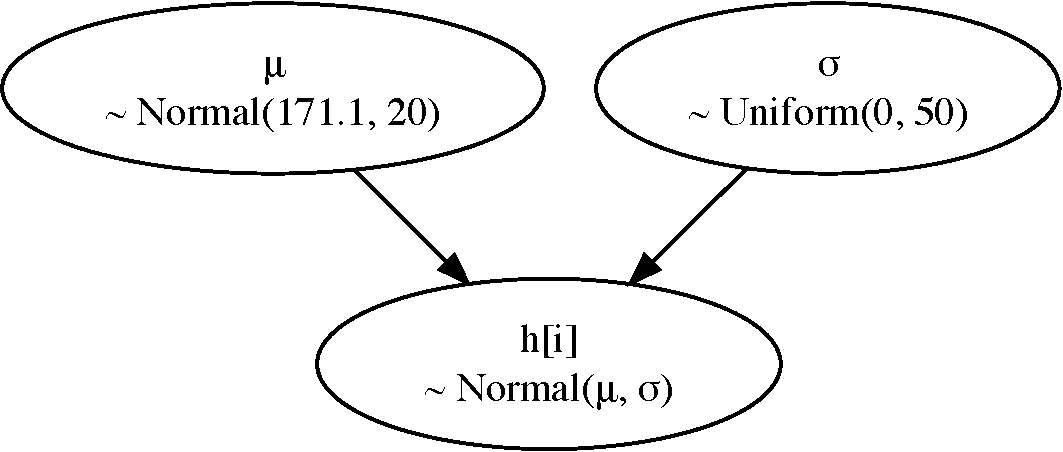
\includegraphics[keepaspectratio]{bookdown-demo_files/figure-latex/unnamed-chunk-4-1.pdf}}

A wide range of population means is possible. Once could discuss this distribution
and maybe further restrict it.

The \textbf{prior for \(\sigma\)} is uniform between \(0\) and \(50\) cm. This is a very wide prior and
just constrains the values to be positive and below \(50\) cm.
This could be stronger of course.

\textbf{Visualization of the prior for \(\sigma\)}:

\begin{Shaded}
\begin{Highlighting}[]
\FunctionTok{curve}\NormalTok{(}\FunctionTok{dunif}\NormalTok{(x, }\DecValTok{0}\NormalTok{, }\DecValTok{50}\NormalTok{), }\AttributeTok{from =} \SpecialCharTok{{-}}\DecValTok{10}\NormalTok{, }\AttributeTok{to =} \DecValTok{60}\NormalTok{)}
\end{Highlighting}
\end{Shaded}

\pandocbounded{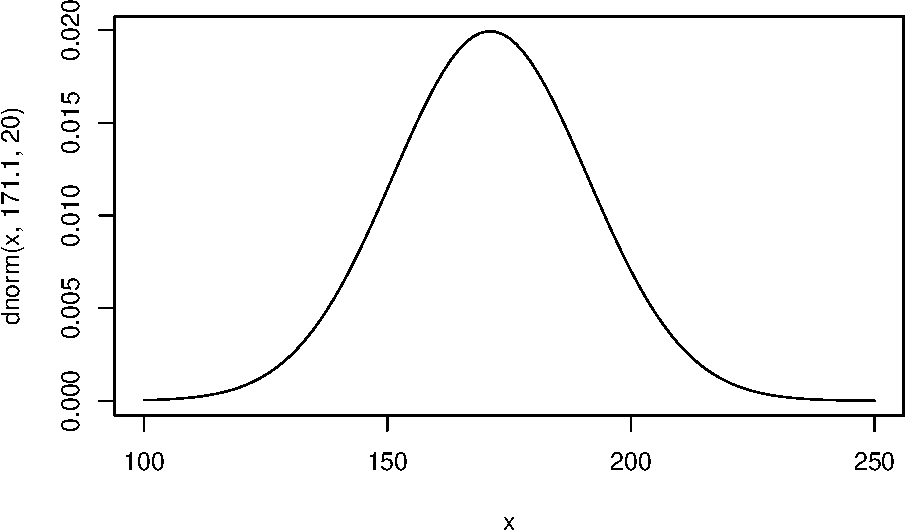
\includegraphics[keepaspectratio]{bookdown-demo_files/figure-latex/unnamed-chunk-5-1.pdf}}

Note, we didn't specify a prior probability distribution of heights
directly, but once we've chosen priors for \(\mu\) and \(\sigma\), these imply a
prior distribution of individual heights.

\textbf{Without} even having seen the \textbf{new data}, we can check what our prior
(model) for heights would predict. This is important. If the prior already
predicts impossible values, we should reconsider our priors and/or model.

So, we simply draw \(\mu\) and \(\sigma\) from the priors and then draw heights
from the normal distribution using the drawn parameters.

\textbf{Vizualisation of the prior for heights}:

\begin{Shaded}
\begin{Highlighting}[]
\NormalTok{sample\_mu }\OtherTok{\textless{}{-}} \FunctionTok{rnorm}\NormalTok{(}\DecValTok{10}\SpecialCharTok{\^{}}\DecValTok{4}\NormalTok{, }\FloatTok{171.1}\NormalTok{, }\DecValTok{20}\NormalTok{)}
\NormalTok{sample\_sigma }\OtherTok{\textless{}{-}} \FunctionTok{runif}\NormalTok{(}\DecValTok{10}\SpecialCharTok{\^{}}\DecValTok{4}\NormalTok{, }\DecValTok{0}\NormalTok{, }\DecValTok{50}\NormalTok{)}
\NormalTok{prior\_h }\OtherTok{\textless{}{-}} \FunctionTok{rnorm}\NormalTok{(}\DecValTok{10}\SpecialCharTok{\^{}}\DecValTok{4}\NormalTok{, sample\_mu, sample\_sigma)}
\FunctionTok{length}\NormalTok{(prior\_h)}
\end{Highlighting}
\end{Shaded}

\begin{verbatim}
## [1] 10000
\end{verbatim}

\begin{Shaded}
\begin{Highlighting}[]
\FunctionTok{dens}\NormalTok{(prior\_h)}
\end{Highlighting}
\end{Shaded}

\pandocbounded{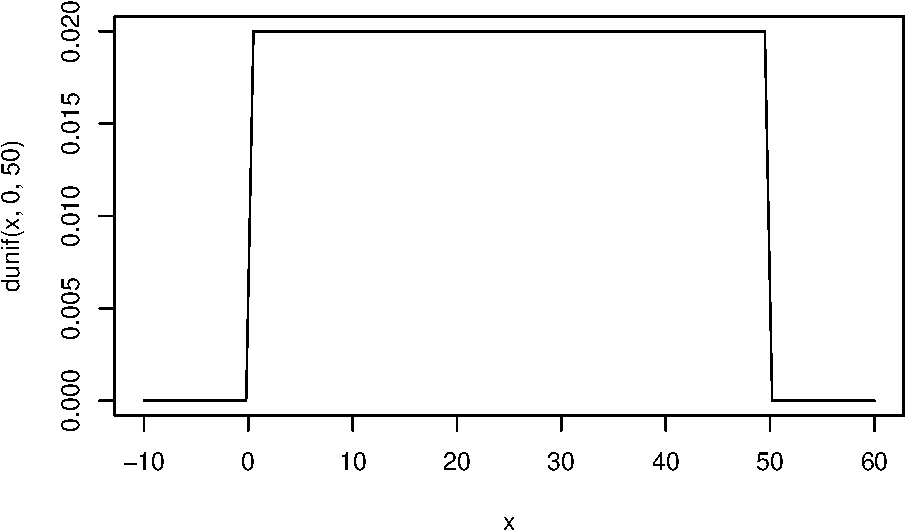
\includegraphics[keepaspectratio]{bookdown-demo_files/figure-latex/unnamed-chunk-6-1.pdf}}

The prior is not itself a Gaussian distribution, but a distribution of
relative plausibilities of different heights, before seeing the data.

Now, there are a couple of different ways to estimtate the model incorporating
the new data. For didactic reasons, grid approximation is often used (as in the book).
For many parameters, this approach becomes more and more infeasible (due to combinatorial explosion).

We will skip that for now and use quadratic approximation instead which
works well for many common procedures in applied statistics (like linear regression).
Later, you'll probably use (or the software in the background) mostly Markov
chain Monte Carlo (MCMC) sampling to get the posterior.
\href{https://civil.colorado.edu/~balajir/CVEN6833/bayes-resources/RM-StatRethink-Bayes.pdf}{Pages 39 and the following}
explain the 3 concepts grid approximation, quadratic approximation and MCMC.

In short, \textbf{quadratic approximation} assumes that our posterior distribution
of body heights can be approximated well by a normal distribution,
at least near the peak.

Please read the \hyperref[bivariate_normal]{addendum} to get a clearer picture of
what a bivariate normal distribution is.

Using the library \texttt{rethinking} we can estimate the model using quadratic approximation.
First, we define the model in the \texttt{rethinking} syntax (see R code 4.25 in the book).

\begin{Shaded}
\begin{Highlighting}[]
\FunctionTok{library}\NormalTok{(rethinking)}
\NormalTok{flist }\OtherTok{\textless{}{-}} \FunctionTok{alist}\NormalTok{(}
\NormalTok{  height }\SpecialCharTok{\textasciitilde{}} \FunctionTok{dnorm}\NormalTok{(mu, sigma),}
\NormalTok{  mu }\SpecialCharTok{\textasciitilde{}} \FunctionTok{dnorm}\NormalTok{(}\FloatTok{171.1}\NormalTok{, }\DecValTok{20}\NormalTok{),}
\NormalTok{  sigma }\SpecialCharTok{\textasciitilde{}} \FunctionTok{dunif}\NormalTok{(}\DecValTok{0}\NormalTok{, }\DecValTok{50}\NormalTok{)}
\NormalTok{)}
\end{Highlighting}
\end{Shaded}

Then we estimate/fit the model using quadratic approximation.

\begin{Shaded}
\begin{Highlighting}[]
\NormalTok{m\_heights }\OtherTok{\textless{}{-}} \FunctionTok{quap}\NormalTok{(flist, }\AttributeTok{data =}\NormalTok{ d2)}
\end{Highlighting}
\end{Shaded}

Now let's take a look at the fitted model:
(Note: In the online-version of the book, they used the command \texttt{map} instead of \texttt{quap}.)

The \texttt{precis}function displays concise parameter estimate information
(from the posterior) for an existing model fit.

\begin{Shaded}
\begin{Highlighting}[]
\FunctionTok{precis}\NormalTok{(m\_heights)}
\end{Highlighting}
\end{Shaded}

\begin{verbatim}
##            mean        sd       5.5%      94.5%
## mu    154.60365 0.4119936 153.945203 155.262093
## sigma   7.73132 0.2913847   7.265631   8.197009
\end{verbatim}

Above, we see the mean of the posterior for \(\mu\) \textbf{and} \(\sigma\);
and a \textbf{89\% credible interval} for those parameters.
Note that these are rather tight credible intervals. We are rather confident that the mean is somewhere between
\(154\) and \(155\) cm and the standard deviation is between \(7\) and \(8\) cm.

We can now plot the posterior distribution of the mean (\(\mu\)) and the standard
deviation (\(\sigma\)) separately by drawing from the posterior distribution.

\begin{Shaded}
\begin{Highlighting}[]
\NormalTok{post }\OtherTok{\textless{}{-}} \FunctionTok{extract.samples}\NormalTok{(m\_heights, }\AttributeTok{n =} \DecValTok{10}\SpecialCharTok{\^{}}\DecValTok{4}\NormalTok{)}
\FunctionTok{head}\NormalTok{(post)}
\end{Highlighting}
\end{Shaded}

\begin{verbatim}
##         mu    sigma
## 1 155.0443 7.523394
## 2 154.8819 7.810746
## 3 154.2174 7.743306
## 4 154.6609 7.780407
## 5 154.4437 7.924487
## 6 154.2984 8.052071
\end{verbatim}

\begin{Shaded}
\begin{Highlighting}[]
\FunctionTok{dens}\NormalTok{(post}\SpecialCharTok{$}\NormalTok{mu)}
\end{Highlighting}
\end{Shaded}

\pandocbounded{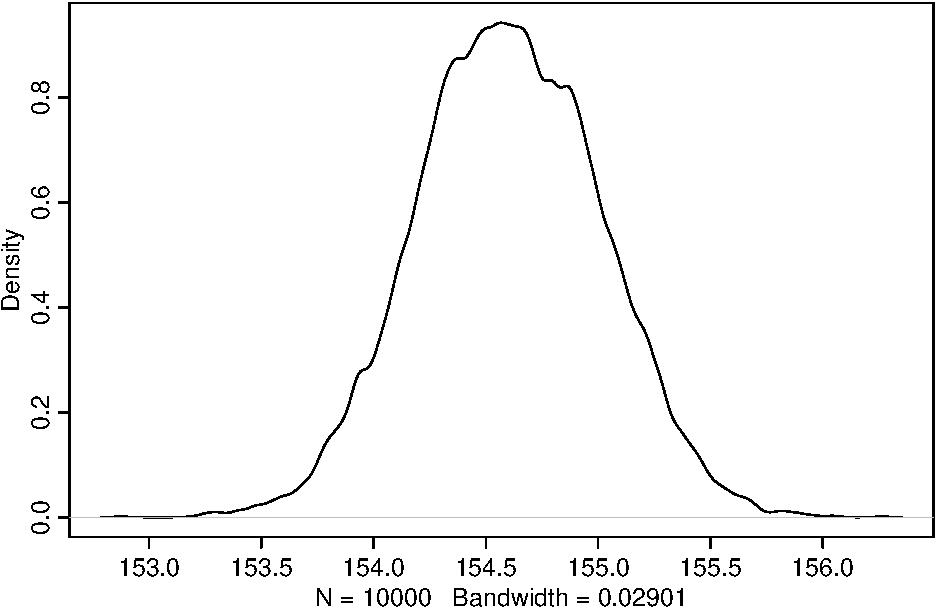
\includegraphics[keepaspectratio]{bookdown-demo_files/figure-latex/unnamed-chunk-10-1.pdf}}

\begin{Shaded}
\begin{Highlighting}[]
\FunctionTok{dens}\NormalTok{(post}\SpecialCharTok{$}\NormalTok{sigma)}
\end{Highlighting}
\end{Shaded}

\pandocbounded{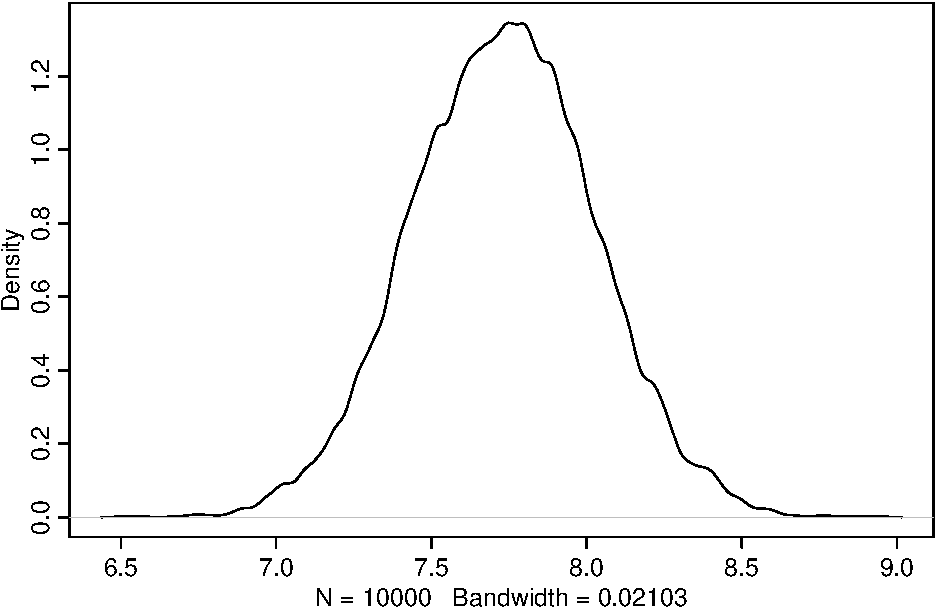
\includegraphics[keepaspectratio]{bookdown-demo_files/figure-latex/unnamed-chunk-10-2.pdf}}

Note, that \textbf{these samples come from a multi-dimensional posterior distribution}.
In our case, we approximated the \textbf{joint} posterior distribution of \(\mu\) \emph{and} \(\sigma\) with a
\href{https://en.wikipedia.org/wiki/Multivariate_normal_distribution}{bivariate normal distribution}.
They are not necessarily independent from each other, but in this case they are.
We know this from the prior definition above. \(\mu\) and \(\sigma\) are both
defined as normal respectively uniform distributions and by definition do not
influence each other. This is also visible in the vizualisation of the model structure:
There is no confounding variable or connection between those priors. One could
think of a common variable \(Z\) that influences both \(\mu\) and \(\sigma\). This could
be genetic similarity which could influence both \(\mu\) and \(\sigma\).

Let's verify that \(\mu\) and \(\sigma\) are uncorrelated:

\begin{Shaded}
\begin{Highlighting}[]
\FunctionTok{vcov}\NormalTok{(m\_heights)}
\end{Highlighting}
\end{Shaded}

\begin{verbatim}
##                 mu        sigma
## mu    0.1697387217 0.0001439151
## sigma 0.0001439151 0.0849050480
\end{verbatim}

gives you the variance-covariance matrix of the parameters of the posterior
distribution. In the diagonal you see the variance of the parameters.

\begin{Shaded}
\begin{Highlighting}[]
\FunctionTok{diag}\NormalTok{(}\FunctionTok{vcov}\NormalTok{(m\_heights))}
\end{Highlighting}
\end{Shaded}

\begin{verbatim}
##         mu      sigma 
## 0.16973872 0.08490505
\end{verbatim}

And we can compute the correlation matrix easily:

\begin{Shaded}
\begin{Highlighting}[]
\FunctionTok{cov2cor}\NormalTok{(}\FunctionTok{vcov}\NormalTok{(m\_heights))}
\end{Highlighting}
\end{Shaded}

\begin{verbatim}
##                mu       sigma
## mu    1.000000000 0.001198807
## sigma 0.001198807 1.000000000
\end{verbatim}

Let's plot the posterior in 3D, because we \textbf{can}:

\pandocbounded{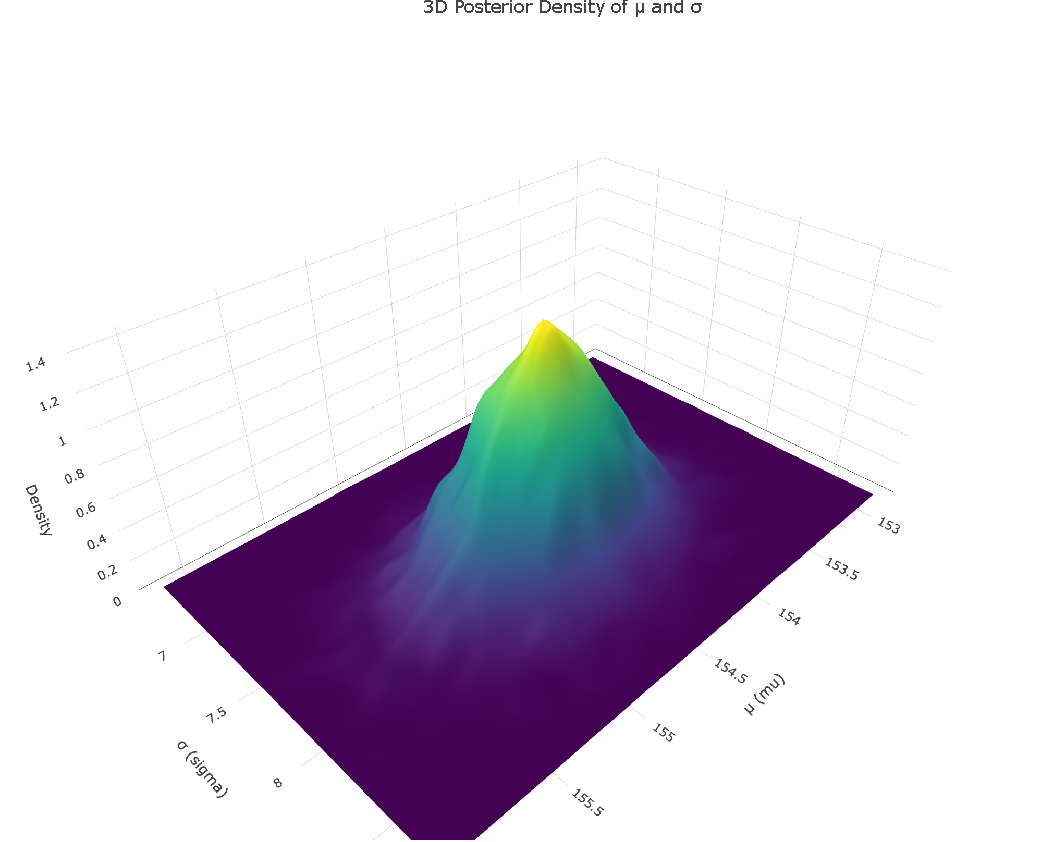
\includegraphics[keepaspectratio]{bookdown-demo_files/figure-latex/posterior-3d-correct-1.pdf}}

\textbf{How beautiful ist that?}

This shows how credible each combination of \(\mu\) and \(\sigma\) is based on our priors and the data observed.
The higher the mountain for a certain parameter combination, the more credible this combination is.

We see in the 3D plot, that the ``mountain'' is not rotated, indicating
graphically that the parameters are independent from each other.

We also see in the correlation matrix, the correlation of the parameters is \(\sim 0\).
In the \href{https://en.wikipedia.org/wiki/Correlation\#Correlation_and_independence}{context of a joint normal distribution},
this means that the parameters are independent.

And, it is not an accident that the posterior looks like this. Using quadratic approximation,
we used the bivariate normal distribution to \textbf{approximate} the posterior.

\section{Classical approach for the simplest model}\label{classical-approach-for-the-simplest-model}

We have seen, how we could use domain and prior knowledge to fit a very simple model
for body heights of a population (!Kung San) in the Bayesian framework.

Now, let's start at the same point in the classical framework.
Here, we do not use any prior knowledge, at least not that explicitely.

The classical approach to fit a regression line is the so-called
\textbf{\href{https://en.wikipedia.org/wiki/Least_squares}{least squares method}}.

There are hundreds of \href{https://www.youtube.com/results?search_query=linear+regression}{videos online}
explaining this method in great detail
with animations. Maybe watch these videos, when we add a predictor to the mean model,
since most of instructional videos start at the simple linear regression using
two parameters (intercept (\(\beta_0\) or \(\alpha\)) and slope (\(\beta_1\))).

The \textbf{(simple mean-) model} is:

\[ Y_i = height_i = c + \varepsilon_i \]

\begin{itemize}
\tightlist
\item
  for some \(c \in \mathbb{R}\) and
\item
  normally distributed errors \(\varepsilon_i \sim \text{Normal}(0, \sigma)\).
\end{itemize}

The errors \(\varepsilon_i\) are on average zero and have a constant standard deviation of \(\sigma\).
So, we assume there is a fixed, but unknown, constant \(c\) that we want to estimate and we
assume that there is a special sort of error in our model that is normally distributed.
Sometimes there is a large deviation from the true \(c\), sometimes there is a small deviation.
On average, the deviations are zero and the \textbf{errors should also be independent from each other}:
\[ \varepsilon_i \perp \varepsilon_j \text{ for } i \neq j\]
This means that just because I have just observed a large deviation from the true \(c\)
does not mean, that the probability of a large deviation in the next observation is higher/lower.
Note, that we cannot readily define different types of errors in the classical framework.

But what is \(c\)? We determine the shape of the model
ourselves (constant model, or mean model) and then estimate the parameter \(c\).
By defining the shape of the model ourselves and imposing a distribution where we want to
estimate the parameter of said distribution, we are in \textbf{parametric statistics}.

We choose the \(c\) which minimizes the sum of squared errors from the actual heights.
This has the advantage that deviations upper and lower from the actual height are
equally weighted. The larger the deviation the (quadratically) larger the penalty.

\textbf{Why do we do that?} Because, if the model assumptions (more on that later)
are correct, the least squares
estimator is a really good estimator. How good? Later\ldots{}

We want to miminize the following function:

\[ SSE \text{ (Sum of Squared Errors) }(c) = (height_1 - c)^2 + (height_2 - c)^2 + 
\ldots + (height_n - c)^2 =\]
\[ = \sum_{i=1}^{n} (height_i - c)^2\]

The SSE is a function of \(c\) and we want to find the \(c\) that minimizes the function.
Since it is a quadratic function, we can always find the minimum.
We have learnt in school how to do this (hopefully): Take the derivative of the function
and set it to zero. Solve for \(c\) and you have the \(c\) which yields the minimum of SSE(c).

Let's do that:

\[ \frac{d}{dc} SSE(c) =  2(height_1 - c)(-1) + 2(height_2 - c)(-1) + 
\ldots + 2(height_n - c)(-1) =\]
\[ = -2 \sum_{i=1}^{n} (height_i - c)\]

This should be zero for the minimum:
\[ -2 \sum_{i=1}^{n} (height_i - c) = 0\]
\[ \sum_{i=1}^{n} (height_i - c) = 0\]
\[ \sum_{i=1}^{n} height_i - n \cdot c = 0\]
\[ \hat{c} = \frac{1}{n} \sum_{i=1}^{n} height_i = \overline{height_i}\]

The hat over the \(c\) indicates that this is the estimated value of \(c\).
Everytime we estimate a parameter, we put a hat over it.

And voilà, we have estimated the parameter \(c\) of the model, which is just the
sample mean of all the heights. In contrast to before, we did not put
in a lot of prior knowledge, but just estimated the parameter from the data.

In R, we can do this easily:

\begin{Shaded}
\begin{Highlighting}[]
\NormalTok{mod }\OtherTok{\textless{}{-}} \FunctionTok{lm}\NormalTok{(height }\SpecialCharTok{\textasciitilde{}} \DecValTok{1}\NormalTok{, }\AttributeTok{data =}\NormalTok{ d2)}
\FunctionTok{summary}\NormalTok{(mod)}
\end{Highlighting}
\end{Shaded}

\begin{verbatim}
## 
## Call:
## lm(formula = height ~ 1, data = d2)
## 
## Residuals:
##      Min       1Q   Median       3Q      Max 
## -18.0721  -6.0071  -0.2921   6.0579  24.4729 
## 
## Coefficients:
##             Estimate Std. Error t value Pr(>|t|)    
## (Intercept) 154.5971     0.4127   374.6   <2e-16 ***
## ---
## Signif. codes:  0 '***' 0.001 '**' 0.01 '*' 0.05 '.' 0.1 ' ' 1
## 
## Residual standard error: 7.742 on 351 degrees of freedom
\end{verbatim}

\begin{Shaded}
\begin{Highlighting}[]
\FunctionTok{dim}\NormalTok{(d2)}
\end{Highlighting}
\end{Shaded}

\begin{verbatim}
## [1] 352   4
\end{verbatim}

\begin{Shaded}
\begin{Highlighting}[]
\FunctionTok{mean}\NormalTok{(d2}\SpecialCharTok{$}\NormalTok{height) }\CommentTok{\# same as the intercept}
\end{Highlighting}
\end{Shaded}

\begin{verbatim}
## [1] 154.5971
\end{verbatim}

\begin{Shaded}
\begin{Highlighting}[]
\FunctionTok{sd}\NormalTok{(d2}\SpecialCharTok{$}\NormalTok{height) }\SpecialCharTok{/} \FunctionTok{sqrt}\NormalTok{(}\FunctionTok{nrow}\NormalTok{(d2)) }\CommentTok{\# standard error of the estimator}
\end{Highlighting}
\end{Shaded}

\begin{verbatim}
## [1] 0.4126677
\end{verbatim}

\begin{Shaded}
\begin{Highlighting}[]
\CommentTok{\# test{-}statistic for the intercept:}
\FunctionTok{mean}\NormalTok{(d2}\SpecialCharTok{$}\NormalTok{height) }\SpecialCharTok{/}\NormalTok{ (}\FunctionTok{sd}\NormalTok{(d2}\SpecialCharTok{$}\NormalTok{height) }\SpecialCharTok{/} \FunctionTok{sqrt}\NormalTok{(}\FunctionTok{nrow}\NormalTok{(d2)))}
\end{Highlighting}
\end{Shaded}

\begin{verbatim}
## [1] 374.6285
\end{verbatim}

\begin{Shaded}
\begin{Highlighting}[]
\CommentTok{\# residual standard error:}
\FunctionTok{sqrt}\NormalTok{(}\FunctionTok{sum}\NormalTok{(mod}\SpecialCharTok{$}\NormalTok{residuals}\SpecialCharTok{\^{}}\DecValTok{2}\NormalTok{) }\SpecialCharTok{/}\NormalTok{ (}\FunctionTok{nrow}\NormalTok{(d2) }\SpecialCharTok{{-}} \DecValTok{1}\NormalTok{))}
\end{Highlighting}
\end{Shaded}

\begin{verbatim}
## [1] 7.742332
\end{verbatim}

The \texttt{\textasciitilde{}1} means that there is just a so-called \textbf{intercept} in the model.
There are \textbf{no covariates}, just the constant \(c\).
This is the simplest we can do. \texttt{lm} stands for linear model and with this base
command in R we ask the software to do the least squares estimation for us.

Let's look at the \textbf{R-output} of the model estimation:

\begin{itemize}
\tightlist
\item
  \texttt{lm(formula\ =\ height\ \textasciitilde{}\ 1,\ data\ =\ d2)}: This is the model we estimated.
\item
  \texttt{Residuals}: The difference between the actual height and the estimated height:
  \(r_i = height_i - \hat{c}\). A univariate 5-point summary is given.
\item
  \texttt{Coefficients}: The estimated coefficients of the model. In this case, there is just the intercept.
  We get the

  \begin{itemize}
  \tightlist
  \item
    \texttt{Std.\ Error} of the estimate, i.e.~the \href{https://en.wikipedia.org/wiki/Standard_error}{standard error} of the mean,
    which is (according to the Central Limit Theorem)
    \[\frac{\sigma}{\sqrt{n}}\] and can be estimated by the sample
    standard deviation divided by the square root of the sample size.
  \item
    the \texttt{t\ value} and the \texttt{Pr(\textgreater{}\textbar{}t\textbar{})} which is the \(p\)-value of the (Wald-)test of
    the null hypothesis that the
    coefficient is zero (\(H_0: \text{intercept}=0\)).
    This is a perfect example of an absolutely useless \(t\)-test.
    Why? Because obviously (\hyperref[exercise2_Intro]{exercise 2}) the population mean of body heights is not zero.
  \end{itemize}
\item
  \texttt{Residual\ standard\ error}: The standard deviation of the residuals \(r_i = height_i - \hat{c}\).
  In this case identical with the sample standard deviation
  of heights (\hyperref[exercise3_Intro]{exercise 3}). \(351\) degrees of freedom. There are \(352\) observations and
  \(1\) parameter estimated (intercept/mean). Hence, there are \(352-1=351\)
  freely movable variables in the statistic of the sample standard deviation.
\end{itemize}

Let's look at the situation graphically:

\pandocbounded{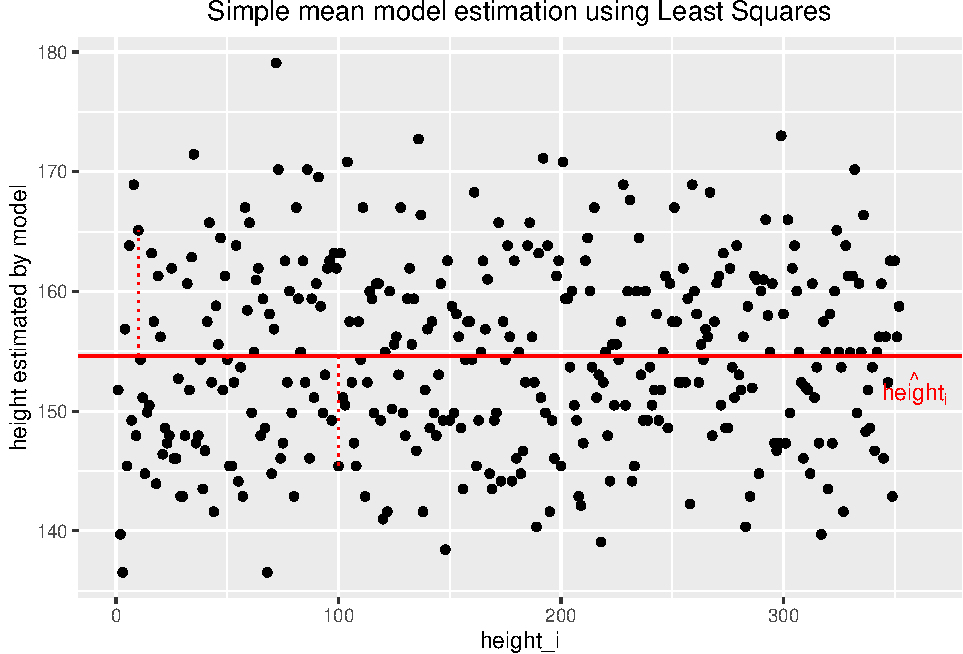
\includegraphics[keepaspectratio]{bookdown-demo_files/figure-latex/unnamed-chunk-15-1.pdf}}

Above, the heights are plotted against the index of the observation (the order does not matter).
The variability of heights around the regression line (constant in this case) seems to
stay constant, which is a good sign. We will call this
\href{https://en.wikipedia.org/wiki/Homoscedasticity_and_heteroscedasticity}{\textbf{homoscedasticity}} later.
The dashed vertical red lines show two residuals (one \(>0\), the other \(<0\)), the difference between the actual height
and the estimated height. The model-estimated heights (\(\widehat{heights_i}\))
are all identical and nothing but the mean of all heights.

Peter Westfall explains in his excellent book a conditional distribution
approach to regression. I highly recommend reading the first chapters.

\textbf{What does this mean in this context?}
This means, that for every fixed value of the predictor (which we formally do not have),
the distribution of the response is normal with mean \(\hat{c}\) and standard deviation \(\sigma\).
Since, we do not have a predictor, we can say, that the distribution of the heights is normal with mean \(\hat{c}\)
and standard deviation \(\sigma\). This is what we assumed in the model. It can also directly seen
in the formula:

\[ height_i = c + \varepsilon_i \]

If you add a normally distributed random variable (\(\varepsilon_i\)) to a constant (\(c\)),
the result is a normally distributed. No surprise here.

\section{Exercises}\label{exercises}

\subsection{{[}E{]} Exercise 1}\label{exercise1_Intro}

Use the \href{https://www.bfs.admin.ch/asset/de/30305714}{Swiss body heights} data to
determine

\begin{itemize}
\tightlist
\item
  the 95\% ``Vertrauensintervall'' for \(\mu\) and
\item
  calculate the standard deviation of the heights from \(21,873\) Swiss people.
\item
  Read the definition of the confidence interval in the footer of the table and
  explain why this is correct.
\end{itemize}

\subsection{{[}E{]} Exercise 2}\label{exercise2_Intro}

Why do we \textbf{not} need a hypothesis test to know that the population mean of body heights is not zero?
Give 2 reasons.

\subsection{{[}M{]} Exercise 3}\label{exercise3_Intro}

Verify analytically that the \texttt{Residual\ standard\ error} is identical with
the sample standard deviation of the heights.

\subsection{{[}M{]} Exercise 4}\label{exercise4_Intro}

Repeat the Bayesian and frequentist estimation of the simple model using a different data set about
\href{https://stat.ethz.ch/R-manual/R-devel/library/datasets/html/ChickWeight.html}{chicken weights},
which is included in R.

\begin{itemize}
\tightlist
\item
  Set useful priors for the mean and standard deviation of the model
  for the Baysian and the frequentist version considering
  your a priori knowledge about chicken weights.
\end{itemize}

\subsection{{[}M{]} Exercise 5}\label{exercise5_Intro}

Try to verify the simulation of probability in the \hyperref[addendum]{addendum} below.

\section{Addendum}\label{addendum}

\subsection{The bivariate normal distribution}\label{bivariate_normal}

As a refresher, you can look into the old QM1 script and read the
chapter ``4.7 Gemeinsame Verteilungen''.
Maybe \href{https://www.youtube.com/watch?v=SP2GKq8xJ5I&ab_channel=StatisticsNinja}{this video}
also helps.

The bivariate normal distribution is a generalization of the normal distribution to two dimensions.
Now, we look at the distribution of two random variables \(X\) and \(Y\) \textbf{at the same time}.

Instead of one Gaussian curve, we have a
\href{https://en.wikipedia.org/wiki/Multivariate_normal_distribution\#/media/File:Multivariate_Gaussian.png}{3D curve}.
This curve defines how plausible different combinations of \(X\) and \(Y\) are.

Single points (like (3,6)) still have probability zero, because now the \textbf{volume} over a single point
(\(x\), \(y\)) is zero. The probability of a certain area is now the \textbf{volume} under the
curve compared to the \textbf{area} under the density curve in the one-dimensional case.

\textbf{Example}: The following plot shows the density of a bivariate normal distribution of
two variables \(X\) and \(Y\)
with \(\mu_X = 0\), \(\mu_Y = 0\), \(\sigma_X = 1\), \(\sigma_Y = 1\) and \(\rho = \frac{2}{3}\).

Below is the correlation matrix of the bivariate normal distribution.

\begin{verbatim}
##           [,1]      [,2]
## [1,] 1.0000000 0.6666667
## [2,] 0.6666667 1.0000000
\end{verbatim}

\pandocbounded{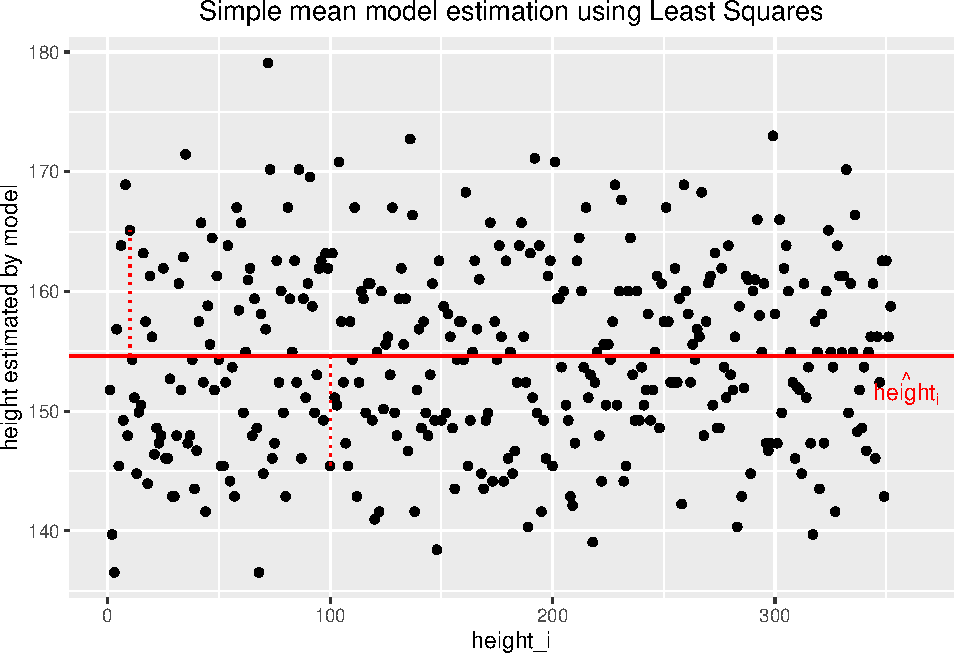
\includegraphics[keepaspectratio]{bookdown-demo_files/figure-latex/unnamed-chunk-16-1.pdf}}

If you move the plot around with your mouse, you see that there is a positive
correlation between \(X\) and \(Y\) (\(\rho = \frac{2}{3}\)). This means that if \(X\) is
above its mean, \(Y\) is also more likely to be above its mean.
The variances of \(X\) and \(Y\) are both \(1\). That means, that if you cut
through the plot in \(X=0\) or \(Y=0\), you see the same form of normal distribution.
If you look at if from above, we have hihglighted the section on the surface
over the area \(X \in [0.5, 2]\) and \(Y \in [0.5, 2]\). The volume over this area
under the density curve is the probability of this area: \(P(X \in [0.5, 2] \text{ and } Y \in [0.5, 2])\)

Calculate with R this probability with R:

\begin{Shaded}
\begin{Highlighting}[]
\CommentTok{\# Load the mvtnorm package}
\FunctionTok{library}\NormalTok{(mvtnorm)}

\CommentTok{\# Define the parameters of the bivariate normal distribution}
\NormalTok{mu }\OtherTok{\textless{}{-}} \FunctionTok{c}\NormalTok{(}\DecValTok{0}\NormalTok{, }\DecValTok{0}\NormalTok{)                       }\CommentTok{\# Mean}
\NormalTok{sigma }\OtherTok{\textless{}{-}} \FunctionTok{matrix}\NormalTok{(}\FunctionTok{c}\NormalTok{(}\FloatTok{0.75}\NormalTok{, }\FloatTok{0.5}\NormalTok{, }\FloatTok{0.5}\NormalTok{, }\FloatTok{0.75}\NormalTok{), }\AttributeTok{ncol =} \DecValTok{2}\NormalTok{) }\CommentTok{\# Covariance matrix}

\CommentTok{\# Define the bounds of the square}
\NormalTok{highlight\_x }\OtherTok{\textless{}{-}} \FunctionTok{c}\NormalTok{(}\FloatTok{0.5}\NormalTok{, }\DecValTok{2}\NormalTok{)}
\NormalTok{highlight\_y }\OtherTok{\textless{}{-}} \FunctionTok{c}\NormalTok{(}\FloatTok{0.5}\NormalTok{, }\DecValTok{2}\NormalTok{)}
\CommentTok{\# Calculate the probability using pmvnorm}
\FunctionTok{pmvnorm}\NormalTok{(}
  \AttributeTok{lower =} \FunctionTok{c}\NormalTok{(highlight\_x[}\DecValTok{1}\NormalTok{], highlight\_y[}\DecValTok{1}\NormalTok{]),}
  \AttributeTok{upper =} \FunctionTok{c}\NormalTok{(highlight\_x[}\DecValTok{2}\NormalTok{], highlight\_y[}\DecValTok{2}\NormalTok{]),}
  \AttributeTok{mean =}\NormalTok{ mu,}
  \AttributeTok{sigma =}\NormalTok{ sigma}
\NormalTok{)}
\end{Highlighting}
\end{Shaded}

\begin{verbatim}
## [1] 0.1526031
## attr(,"error")
## [1] 1e-15
## attr(,"msg")
## [1] "Normal Completion"
\end{verbatim}

Since we do not believe everything we are told, we rather check via simulation,
if \(0.1526\) is a plausible value for the probability:

\begin{Shaded}
\begin{Highlighting}[]
\CommentTok{\# Load necessary library}
\FunctionTok{library}\NormalTok{(MASS)}

\CommentTok{\# Define the parameters of the bivariate normal distribution}
\NormalTok{mu }\OtherTok{\textless{}{-}} \FunctionTok{c}\NormalTok{(}\DecValTok{0}\NormalTok{, }\DecValTok{0}\NormalTok{)                       }\CommentTok{\# Mean}
\NormalTok{sigma }\OtherTok{\textless{}{-}} \FunctionTok{matrix}\NormalTok{(}\FunctionTok{c}\NormalTok{(}\FloatTok{0.75}\NormalTok{, }\FloatTok{0.5}\NormalTok{, }\FloatTok{0.5}\NormalTok{, }\FloatTok{0.75}\NormalTok{), }\AttributeTok{ncol =} \DecValTok{2}\NormalTok{) }\CommentTok{\# Covariance matrix}

\CommentTok{\# Define the bounds of the square}
\NormalTok{highlight\_x }\OtherTok{\textless{}{-}} \FunctionTok{c}\NormalTok{(}\FloatTok{0.5}\NormalTok{, }\DecValTok{2}\NormalTok{)}
\NormalTok{highlight\_y }\OtherTok{\textless{}{-}} \FunctionTok{c}\NormalTok{(}\FloatTok{0.5}\NormalTok{, }\DecValTok{2}\NormalTok{)}

\CommentTok{\# Number of simulations}
\NormalTok{n\_sim }\OtherTok{\textless{}{-}} \DecValTok{10}\SpecialCharTok{\^{}}\DecValTok{4}

\FunctionTok{set.seed}\NormalTok{(}\DecValTok{343434}\NormalTok{)}
\CommentTok{\# Simulate bivariate normal samples}
\NormalTok{samples }\OtherTok{\textless{}{-}} \FunctionTok{mvrnorm}\NormalTok{(}\AttributeTok{n =}\NormalTok{ n\_sim, }\AttributeTok{mu =}\NormalTok{ mu, }\AttributeTok{Sigma =}\NormalTok{ sigma)}

\CommentTok{\# Count how many samples fall within the square}
\NormalTok{inside\_square }\OtherTok{\textless{}{-}} \FunctionTok{sum}\NormalTok{(}
\NormalTok{  samples[, }\DecValTok{1}\NormalTok{] }\SpecialCharTok{\textgreater{}=}\NormalTok{ highlight\_x[}\DecValTok{1}\NormalTok{] }\SpecialCharTok{\&}\NormalTok{ samples[, }\DecValTok{1}\NormalTok{] }\SpecialCharTok{\textless{}=}\NormalTok{ highlight\_x[}\DecValTok{2}\NormalTok{] }\SpecialCharTok{\&}
\NormalTok{  samples[, }\DecValTok{2}\NormalTok{] }\SpecialCharTok{\textgreater{}=}\NormalTok{ highlight\_y[}\DecValTok{1}\NormalTok{] }\SpecialCharTok{\&}\NormalTok{ samples[, }\DecValTok{2}\NormalTok{] }\SpecialCharTok{\textless{}=}\NormalTok{ highlight\_y[}\DecValTok{2}\NormalTok{]}
\NormalTok{)}

\CommentTok{\# Estimate the probability}
\NormalTok{inside\_square }\SpecialCharTok{/}\NormalTok{ n\_sim}
\end{Highlighting}
\end{Shaded}

\begin{verbatim}
## [1] 0.1557
\end{verbatim}

Looks good.

\chapter{Simple Linear Regression}\label{simple-linear-regression}

\section{Simple Linear Regression in the Bayesian Framework}\label{simple-linear-regression-in-the-bayesian-framework}

We will now add one covariate/explanatory variable to the model.
Refer to \href{https://civil.colorado.edu/~balajir/CVEN6833/bayes-resources/RM-StatRethink-Bayes.pdf}{Statistical Rethinking}
``4.4 Linear prediction'' or ``4.4 Adding a predictor'' as it's called in the online version of the book.

So far, our ``regression'' did not do much to be honest. The mean of a list of values
was already calculated in the \href{https://jdegenfellner.github.io/Script_QM1_ZHAW/descriptive_stats.html}{descriptive statistics section}
before and we have mentioned how great this statistic is as measure of location and where its weaknesses are.

Now, we want to model \textbf{how} body height and weight are \textbf{related}.
Formally, one wants to \emph{predict} body heights from body weights.

Here and in the frequentist framework, we will see that it is \textbf{not the same}
problem (and therefore results in a different statistical model)
\textbf{to predict body weights from body heights or vice versa}.

The word ``predictor'' is important here. It is a technical term
and describes a variable that we know (in our case weight) and with
which we want to ``guess as good as possible'' the value of the
dependent variable (in our case height). ``As good as possible''
means that we put a penalty on an error. The farer our prediction
is aways from the true value (\(y_i\)), the higher the penalty.
And not only that, but if you are twice as far away from the true value,
you should be penalized four times as much. This is the idea behind
the squared error \href{https://en.wikipedia.org/wiki/Loss_function}{loss function}
and the core of the least squares method.
What if we would punish differently you ask?
There are many loss functions one could use, maybe we will see some
later. For now, we punish quadratically.

We \textbf{always} visualize the data first to improve our understanding.

\begin{Shaded}
\begin{Highlighting}[]
\FunctionTok{plot}\NormalTok{(d2}\SpecialCharTok{$}\NormalTok{height }\SpecialCharTok{\textasciitilde{}}\NormalTok{ d2}\SpecialCharTok{$}\NormalTok{weight)}
\end{Highlighting}
\end{Shaded}

\pandocbounded{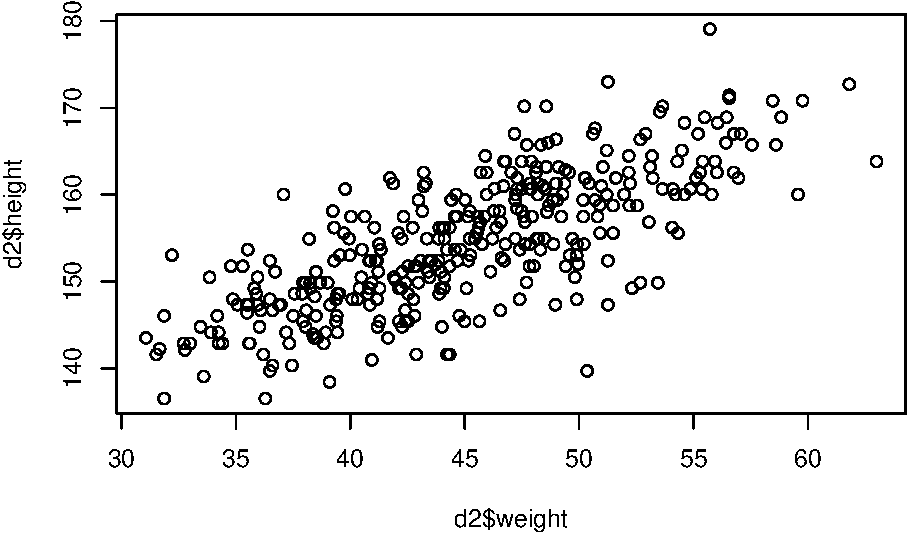
\includegraphics[keepaspectratio]{bookdown-demo_files/figure-latex/unnamed-chunk-19-1.pdf}}

It's not often, that you see such a clean plot.
The scatterplot indicates a linear relationship between the two variables.
The higher the weight, the higher the height; with some deviations of course and
we decide that normally distributed errors are a good idea.
This relationsip is neither causal, nor deterministic.

\begin{itemize}
\tightlist
\item
  It is not causal since an increase in weight does not
  necessarily lead to an increase in height, especially in grown-ups.
\item
  It is not deterministic since there are deviations from the line.
  It if was deterministic, we would not need statistical modeling.
\end{itemize}

For simpler notation, we will call \texttt{d2\$weight} \(x\). \(\bar{x}\)
is the mean of \(x\).

\subsection{Model definition}\label{model-definition}

Let's write down our \textbf{model} (again with the Swiss population prior mean):

\begin{eqnarray*}
h_i &\sim& \text{Normal}(\mu_i, \sigma)\\
\mu_i &\sim& \alpha + \beta (x_i - \bar{x})\\
\alpha &\sim& \text{Normal}(171.1, 20)\\
\beta &\sim& \text{Normal}(0, 10)\\
\sigma &\sim& \text{Uniform}(0, 50)
\end{eqnarray*}

Visualization of the \textbf{model structure}:

\begin{verbatim}
## file:////private/var/folders/pm/jd6n6gj10371_bml1gh8sc5w0000gn/T/RtmpkK6ULT/file57f64a48308/widget57f64c968499.html screenshot completed
\end{verbatim}

\pandocbounded{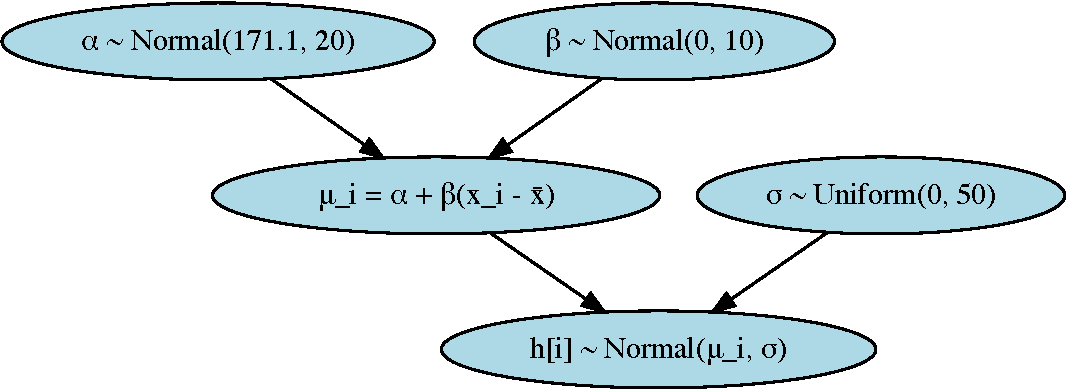
\includegraphics[keepaspectratio]{bookdown-demo_files/figure-latex/unnamed-chunk-20-1.pdf}}

There are now additional lines for the priors of \(\alpha\) and \(\beta\).
The model structure also shows the way to simulate from the prior.
One starts at the top and ends up with the heights.

\begin{itemize}
\tightlist
\item
  \(h_i\) is the height of the \(i\)-th person and we assume it is normally distributed.
\item
  \(\mu_i\) is the mean of the height of the \(i\)-th person and we
  assume it is linearly dependent on the difference \(x_i-\bar{x}\).
  Compared to the intercept model, a different mean is assumed for each person
  depending on his/her weight.
\item
  \(\alpha\) is the intercept and we use the same prior as before.
\item
  \(\beta\) is the slope of the line and we use the normal distribution as prior for it,
  hence it can be positive or negative and how plausible each value is, is
  determined by that specific normal distribution. Note, that we could
  easily adapt the distribtion to any distribution we like.
\item
  The prior for \(\sigma\) is unchanged.
\item
  \(x_i - \bar{x}\) is the deviation of the weight from the mean weight, thereby \textbf{we
  center} the weight variable. This is a common practice in regression analysis.
\end{itemize}

The linear model is quite popular in applied statistics and one
reason is probably the rather straightforward interpretation of the coefficients.

\subsection{Priors}\label{priors}

We want to plot our priors to get a feeling \textbf{what
the model would predict without seeing the data}.
This is a kind of ``sanity check'' to see if the priors are reasonable.
Again, we just draw from the assumed distributions for \(\alpha\) and \(\beta\)
100 times and draw the corresponding lines. Just as the model
definition says.

\begin{Shaded}
\begin{Highlighting}[]
\FunctionTok{set.seed}\NormalTok{(}\DecValTok{2971}\NormalTok{)}
\NormalTok{N }\OtherTok{\textless{}{-}} \DecValTok{100}  \CommentTok{\# 100 lines}
\NormalTok{a }\OtherTok{\textless{}{-}} \FunctionTok{rnorm}\NormalTok{(N, }\FloatTok{171.1}\NormalTok{, }\DecValTok{20}\NormalTok{)}
\NormalTok{b }\OtherTok{\textless{}{-}} \FunctionTok{rnorm}\NormalTok{(N, }\DecValTok{0}\NormalTok{, }\DecValTok{10}\NormalTok{)}

\CommentTok{\# Assume d2$weight is defined, e.g., using some dataset or simulation}
\NormalTok{xbar }\OtherTok{\textless{}{-}} \FunctionTok{mean}\NormalTok{(d2}\SpecialCharTok{$}\NormalTok{weight)}

\FunctionTok{plot}\NormalTok{(}\ConstantTok{NULL}\NormalTok{, }\AttributeTok{xlim =} \FunctionTok{range}\NormalTok{(d2}\SpecialCharTok{$}\NormalTok{weight), }\AttributeTok{ylim =} \FunctionTok{c}\NormalTok{(}\SpecialCharTok{{-}}\DecValTok{100}\NormalTok{, }\DecValTok{400}\NormalTok{),}
     \AttributeTok{xlab =} \StringTok{"weight"}\NormalTok{, }\AttributeTok{ylab =} \StringTok{"height"}\NormalTok{)}
\FunctionTok{abline}\NormalTok{(}\AttributeTok{h =} \DecValTok{0}\NormalTok{, }\AttributeTok{lty =} \DecValTok{2}\NormalTok{)  }\CommentTok{\# horizontal line at 0}
\FunctionTok{abline}\NormalTok{(}\AttributeTok{h =} \DecValTok{272}\NormalTok{, }\AttributeTok{lty =} \DecValTok{1}\NormalTok{, }\AttributeTok{lwd =} \FloatTok{0.5}\NormalTok{)  }\CommentTok{\# horizontal line at 272}
\FunctionTok{mtext}\NormalTok{(}\StringTok{"b \textasciitilde{} dnorm(0, 10)"}\NormalTok{)}

\CommentTok{\# Overlay the 100 lines}
\ControlFlowTok{for}\NormalTok{ (i }\ControlFlowTok{in} \DecValTok{1}\SpecialCharTok{:}\NormalTok{N) \{}
  \FunctionTok{curve}\NormalTok{(a[i] }\SpecialCharTok{+}\NormalTok{ b[i] }\SpecialCharTok{*}\NormalTok{ (x }\SpecialCharTok{{-}}\NormalTok{ xbar),}
        \AttributeTok{from =} \FunctionTok{min}\NormalTok{(d2}\SpecialCharTok{$}\NormalTok{weight), }\AttributeTok{to =} \FunctionTok{max}\NormalTok{(d2}\SpecialCharTok{$}\NormalTok{weight),}
        \AttributeTok{add =} \ConstantTok{TRUE}\NormalTok{, }\AttributeTok{col =} \FunctionTok{col.alpha}\NormalTok{(}\StringTok{"black"}\NormalTok{, }\FloatTok{0.2}\NormalTok{))}
\NormalTok{\}}
\end{Highlighting}
\end{Shaded}

\pandocbounded{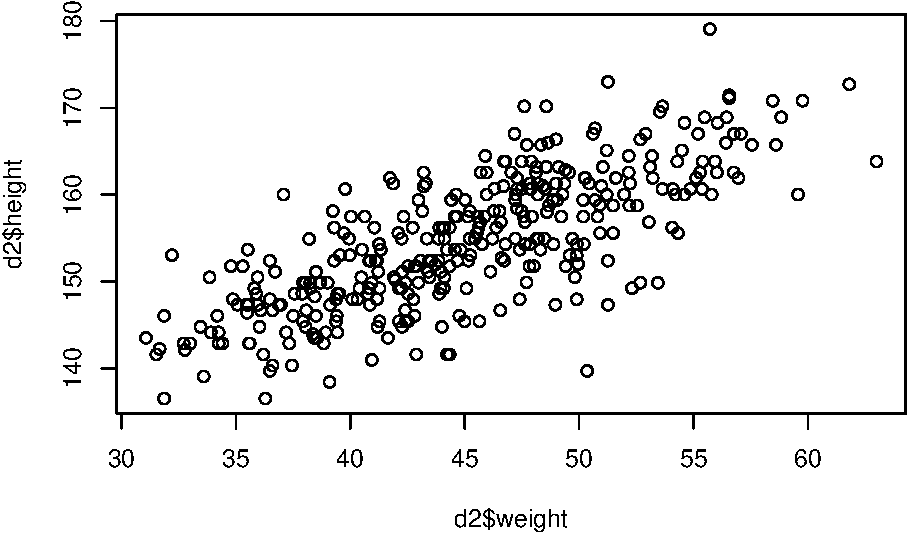
\includegraphics[keepaspectratio]{bookdown-demo_files/figure-latex/unnamed-chunk-21-1.pdf}}

This linear relationship defined with the chosen priors seems rather
non-restrictive. According to our priors,
one could see very steeply rising or falling lines. We could at least make
the priors for the slope (\(\beta\)) non-negative. One possibility to do this
is to use a \href{https://en.wikipedia.org/wiki/Log-normal_distribution}{log-normal distribution}
for the prior of \(\beta\) which can only take non-negative values.

\[ \beta \sim \text{Log-Normal}(0, 1) \]

Lets plot the priors again.

\begin{Shaded}
\begin{Highlighting}[]
\FunctionTok{set.seed}\NormalTok{(}\DecValTok{2971}\NormalTok{)}
\NormalTok{N }\OtherTok{\textless{}{-}} \DecValTok{100}  \CommentTok{\# 100 lines}
\NormalTok{a }\OtherTok{\textless{}{-}} \FunctionTok{rnorm}\NormalTok{(N, }\FloatTok{171.1}\NormalTok{, }\DecValTok{20}\NormalTok{)}
\NormalTok{b }\OtherTok{\textless{}{-}} \FunctionTok{rlnorm}\NormalTok{(N, }\DecValTok{0}\NormalTok{, }\DecValTok{1}\NormalTok{)}

\CommentTok{\# Assume d2$weight is defined, e.g., using some dataset or simulation}
\NormalTok{xbar }\OtherTok{\textless{}{-}} \FunctionTok{mean}\NormalTok{(d2}\SpecialCharTok{$}\NormalTok{weight)}

\FunctionTok{plot}\NormalTok{(}\ConstantTok{NULL}\NormalTok{, }\AttributeTok{xlim =} \FunctionTok{range}\NormalTok{(d2}\SpecialCharTok{$}\NormalTok{weight), }\AttributeTok{ylim =} \FunctionTok{c}\NormalTok{(}\SpecialCharTok{{-}}\DecValTok{100}\NormalTok{, }\DecValTok{400}\NormalTok{),}
     \AttributeTok{xlab =} \StringTok{"weight"}\NormalTok{, }\AttributeTok{ylab =} \StringTok{"height"}\NormalTok{)}
\FunctionTok{abline}\NormalTok{(}\AttributeTok{h =} \DecValTok{0}\NormalTok{, }\AttributeTok{lty =} \DecValTok{2}\NormalTok{)  }\CommentTok{\# horizontal line at 0}
\FunctionTok{abline}\NormalTok{(}\AttributeTok{h =} \DecValTok{272}\NormalTok{, }\AttributeTok{lty =} \DecValTok{1}\NormalTok{, }\AttributeTok{lwd =} \FloatTok{0.5}\NormalTok{)  }\CommentTok{\# horizontal line at 272}
\FunctionTok{mtext}\NormalTok{(}\StringTok{"b \textasciitilde{} dlnorm(0, 1)"}\NormalTok{)}

\CommentTok{\# Overlay the 100 lines}
\ControlFlowTok{for}\NormalTok{ (i }\ControlFlowTok{in} \DecValTok{1}\SpecialCharTok{:}\NormalTok{N) \{}
  \FunctionTok{curve}\NormalTok{(a[i] }\SpecialCharTok{+}\NormalTok{ b[i] }\SpecialCharTok{*}\NormalTok{ (x }\SpecialCharTok{{-}}\NormalTok{ xbar),}
        \AttributeTok{from =} \FunctionTok{min}\NormalTok{(d2}\SpecialCharTok{$}\NormalTok{weight), }\AttributeTok{to =} \FunctionTok{max}\NormalTok{(d2}\SpecialCharTok{$}\NormalTok{weight),}
        \AttributeTok{add =} \ConstantTok{TRUE}\NormalTok{, }\AttributeTok{col =} \FunctionTok{col.alpha}\NormalTok{(}\StringTok{"black"}\NormalTok{, }\FloatTok{0.2}\NormalTok{))}
\NormalTok{\}}
\end{Highlighting}
\end{Shaded}

\pandocbounded{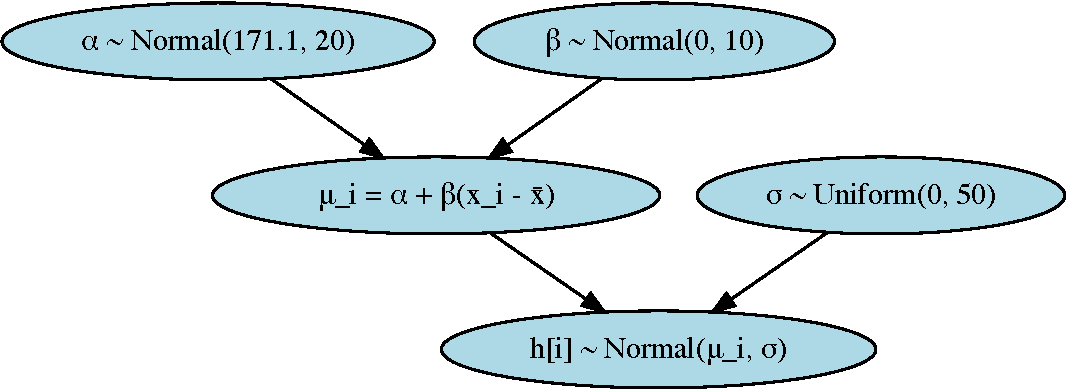
\includegraphics[keepaspectratio]{bookdown-demo_files/figure-latex/unnamed-chunk-22-1.pdf}}

This seems definitely more realistic.

\subsection{Fit model}\label{fit-model}

Now, let's \textbf{estimate the posterior/fit the model} as before:

\begin{Shaded}
\begin{Highlighting}[]
\CommentTok{\# load data again, since it\textquotesingle{}s a long way back}
\FunctionTok{library}\NormalTok{(rethinking)}
\FunctionTok{data}\NormalTok{(Howell1)}
\NormalTok{d }\OtherTok{\textless{}{-}}\NormalTok{ Howell1}
\NormalTok{d2 }\OtherTok{\textless{}{-}}\NormalTok{ d[d}\SpecialCharTok{$}\NormalTok{age }\SpecialCharTok{\textgreater{}=} \DecValTok{18}\NormalTok{, ]}
\NormalTok{xbar }\OtherTok{\textless{}{-}} \FunctionTok{mean}\NormalTok{(d2}\SpecialCharTok{$}\NormalTok{weight)}
\CommentTok{\# fit model}
\NormalTok{mod }\OtherTok{\textless{}{-}} \FunctionTok{quap}\NormalTok{(}
    \FunctionTok{alist}\NormalTok{(}
\NormalTok{        height }\SpecialCharTok{\textasciitilde{}} \FunctionTok{dnorm}\NormalTok{(mu, sigma),}
\NormalTok{        mu }\OtherTok{\textless{}{-}}\NormalTok{ a }\SpecialCharTok{+}\NormalTok{ b }\SpecialCharTok{*}\NormalTok{ (weight }\SpecialCharTok{{-}}\NormalTok{ xbar),}
\NormalTok{        a }\SpecialCharTok{\textasciitilde{}} \FunctionTok{dnorm}\NormalTok{(}\FloatTok{171.1}\NormalTok{, }\DecValTok{100}\NormalTok{),}
\NormalTok{        b }\SpecialCharTok{\textasciitilde{}} \FunctionTok{dnorm}\NormalTok{(}\DecValTok{0}\NormalTok{, }\DecValTok{10}\NormalTok{),}
\NormalTok{        sigma }\SpecialCharTok{\textasciitilde{}} \FunctionTok{dunif}\NormalTok{(}\DecValTok{0}\NormalTok{, }\DecValTok{50}\NormalTok{)}
\NormalTok{    ) ,}
\AttributeTok{data =}\NormalTok{ d2)}
\end{Highlighting}
\end{Shaded}

Let's look at the \textbf{marginal distributions} of the parameters:

\begin{Shaded}
\begin{Highlighting}[]
\FunctionTok{precis}\NormalTok{(mod)}
\end{Highlighting}
\end{Shaded}

\begin{verbatim}
##              mean         sd        5.5%       94.5%
## a     154.5972120 0.27033045 154.1651717 155.0292523
## b       0.9050131 0.04192754   0.8380048   0.9720214
## sigma   5.0718673 0.19115323   4.7663675   5.3773671
\end{verbatim}

The analysis yields estimates for all our parameters of the model: \(\alpha\),
\(\beta\) and \(\sigma\). The estimates are the mean of the posterior distribution.

See \hyperref[exercise2_simpl_lin_reg]{exercise 2}.

\textbf{Interpretation of \(\beta\)}:
The mean of the posterior distribution of \(\beta\) is 0.9. A person with a weight
of 1 kg more weight can be expected to be 0.9 cm taller. A 89\% credible interval
for this estimate is \([0.83, 0.97]\). We can be quite sure that the slope is
positive (of course we designed it that way too via the prior).

It might also be interesting to inspect the \textbf{variance-covariance matrix},
respectively the correlation between the parameters as we did before
in the intercept model. Remember, these are the correlations of
parameters in the multivariate (because three paremeters simulatenously)
posterior distribution.

\begin{Shaded}
\begin{Highlighting}[]
\FunctionTok{diag}\NormalTok{(}\FunctionTok{vcov}\NormalTok{(mod))}
\end{Highlighting}
\end{Shaded}

\begin{verbatim}
##           a           b       sigma 
## 0.073078550 0.001757918 0.036539558
\end{verbatim}

\begin{Shaded}
\begin{Highlighting}[]
\FunctionTok{round}\NormalTok{(}\FunctionTok{cov2cor}\NormalTok{(}\FunctionTok{vcov}\NormalTok{(mod)),}\DecValTok{2}\NormalTok{)}
\end{Highlighting}
\end{Shaded}

\begin{verbatim}
##       a b sigma
## a     1 0     0
## b     0 1     0
## sigma 0 0     1
\end{verbatim}

\begin{itemize}
\tightlist
\item
  \texttt{diag(vcov(mod))} gives the variances of the parameters and
\item
  \texttt{cov2cor(vcov(mod))}the correlations. As we can see the correlations are (near) zero. Compare to the graphical
  display of the model structure. There is no connection.
\end{itemize}

\subsection{Result}\label{result}

\textbf{Graphical end result} of fitting the model:

\begin{Shaded}
\begin{Highlighting}[]
\FunctionTok{plot}\NormalTok{(d2}\SpecialCharTok{$}\NormalTok{height }\SpecialCharTok{\textasciitilde{}}\NormalTok{ d2}\SpecialCharTok{$}\NormalTok{weight, }\AttributeTok{col =}\NormalTok{ rangi2)}
\NormalTok{post }\OtherTok{\textless{}{-}} \FunctionTok{extract.samples}\NormalTok{(mod)}
\NormalTok{a\_quap }\OtherTok{\textless{}{-}} \FunctionTok{mean}\NormalTok{(post}\SpecialCharTok{$}\NormalTok{a)}
\NormalTok{b\_quap }\OtherTok{\textless{}{-}} \FunctionTok{mean}\NormalTok{(post}\SpecialCharTok{$}\NormalTok{b)}
\FunctionTok{curve}\NormalTok{(a\_quap }\SpecialCharTok{+}\NormalTok{ b\_quap }\SpecialCharTok{*}\NormalTok{ (x }\SpecialCharTok{{-}}\NormalTok{ xbar), }\AttributeTok{add =} \ConstantTok{TRUE}\NormalTok{)}
\end{Highlighting}
\end{Shaded}

\pandocbounded{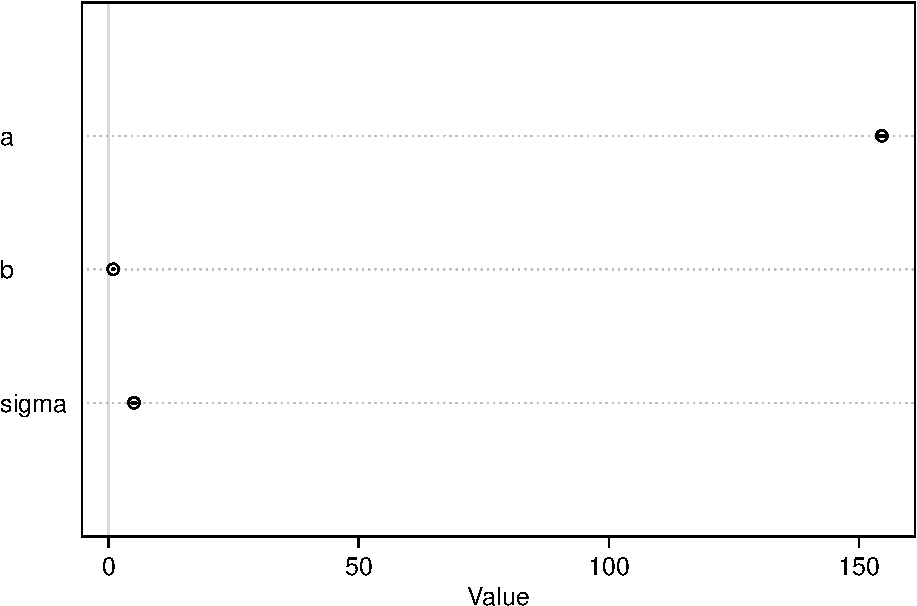
\includegraphics[keepaspectratio]{bookdown-demo_files/figure-latex/unnamed-chunk-26-1.pdf}}

\subsection{Credible bands}\label{credible-bands}

We could draw again and again from the posterior distribution
and calculate the means like above. Plotting the regression lines
with the respective parameters \(\alpha\), \(\beta\) would indicate
the variability of the estimates.

\begin{Shaded}
\begin{Highlighting}[]
\CommentTok{\# Define a sequence of weights for predictions}
\NormalTok{weight.seq }\OtherTok{\textless{}{-}} \FunctionTok{seq}\NormalTok{(}\AttributeTok{from =} \DecValTok{25}\NormalTok{, }\AttributeTok{to =} \DecValTok{70}\NormalTok{, }\AttributeTok{by =} \DecValTok{1}\NormalTok{)}

\CommentTok{\# Use the model to compute mu for each weight}
\NormalTok{mu }\OtherTok{\textless{}{-}} \FunctionTok{link}\NormalTok{(mod, }\AttributeTok{data =} \FunctionTok{data.frame}\NormalTok{(}\AttributeTok{weight =}\NormalTok{ weight.seq))}
\FunctionTok{str}\NormalTok{(mu)}
\end{Highlighting}
\end{Shaded}

\begin{verbatim}
##  num [1:1000, 1:46] 138 136 137 136 137 ...
\end{verbatim}

\begin{Shaded}
\begin{Highlighting}[]
\CommentTok{\# Visualize the distribution of mu values}
\FunctionTok{plot}\NormalTok{(height }\SpecialCharTok{\textasciitilde{}}\NormalTok{ weight, d2, }\AttributeTok{type =} \StringTok{"n"}\NormalTok{)  }\CommentTok{\# Hide raw data with type = "n"}

\CommentTok{\# Loop over samples and plot each mu value}
\ControlFlowTok{for}\NormalTok{ (i }\ControlFlowTok{in} \DecValTok{1}\SpecialCharTok{:}\DecValTok{100}\NormalTok{) \{}
  \FunctionTok{points}\NormalTok{(weight.seq, mu[i, ], }\AttributeTok{pch =} \DecValTok{16}\NormalTok{, }\AttributeTok{col =} \FunctionTok{col.alpha}\NormalTok{(rangi2, }\FloatTok{0.1}\NormalTok{))}
\NormalTok{\}}
\end{Highlighting}
\end{Shaded}

\pandocbounded{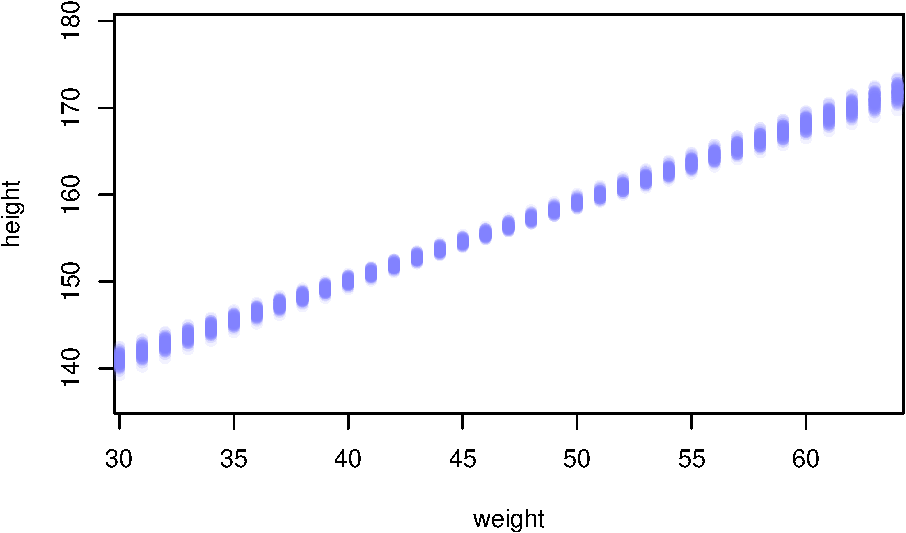
\includegraphics[keepaspectratio]{bookdown-demo_files/figure-latex/unnamed-chunk-27-1.pdf}}

The \texttt{link} function fixes the weight at the values in \texttt{weight.seq} and
draws samples from the posterior distribution of the parameters. We will do
the analog thing in the frequentist framework.

We can also draw a nice shade for the regression line:

\begin{Shaded}
\begin{Highlighting}[]
\CommentTok{\# Summarize the distribution of mu}
\NormalTok{mu.mean }\OtherTok{\textless{}{-}} \FunctionTok{apply}\NormalTok{(mu, }\DecValTok{2}\NormalTok{, mean)}
\NormalTok{mu.PI }\OtherTok{\textless{}{-}} \FunctionTok{apply}\NormalTok{(mu, }\DecValTok{2}\NormalTok{, PI, }\AttributeTok{prob =} \FloatTok{0.89}\NormalTok{)}
\FunctionTok{plot}\NormalTok{(height }\SpecialCharTok{\textasciitilde{}}\NormalTok{ weight, d2, }\AttributeTok{col =} \FunctionTok{col.alpha}\NormalTok{(rangi2, }\FloatTok{0.5}\NormalTok{))}
\FunctionTok{lines}\NormalTok{(weight.seq, mu.mean)}
\FunctionTok{shade}\NormalTok{(mu.PI, weight.seq)}
\end{Highlighting}
\end{Shaded}

\pandocbounded{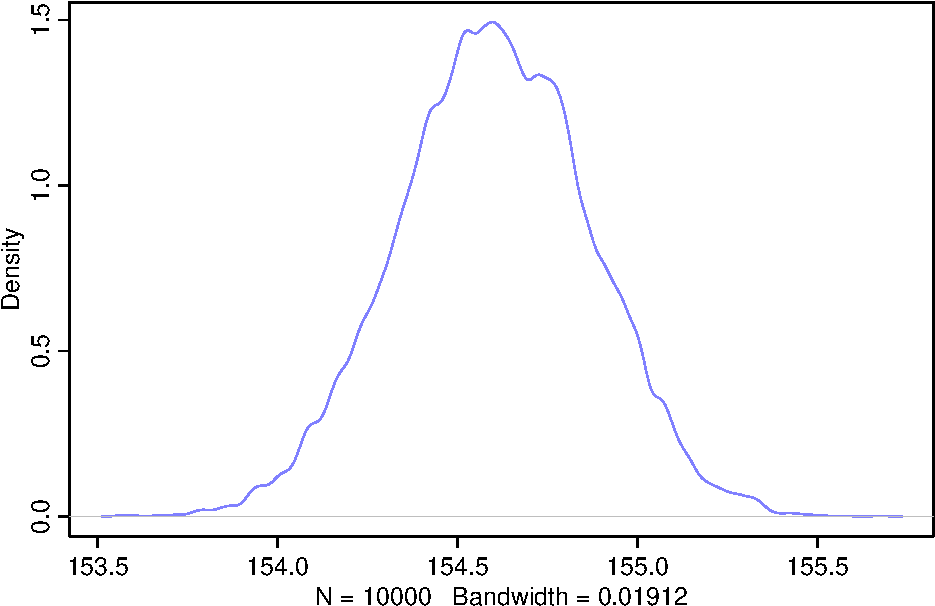
\includegraphics[keepaspectratio]{bookdown-demo_files/figure-latex/unnamed-chunk-28-1.pdf}}

As we can see, we are pretty sure about the mean of height which
we wanted to model in the first place.
\textbf{Mean modeling is one thing, individual prediction is another}.
Given a certain weight of a person, what is the height of the same person?
The first line in the model definition (\(height_i \sim Normal(\mu_i, \sigma)\))
tells us that a person's weight is distributed \emph{around} the mean
(which linearly depends on weight) and is not necessary the mean itself.

To get to an \textbf{individual prediction}, we need to consider the uncertainty
of the parameter estimation \emph{and} the uncertainty from the Gaussian distribution
around the mean (at a certain weight). We do this with \texttt{sim}.

\begin{Shaded}
\begin{Highlighting}[]
\CommentTok{\# Simulate heights from the posterior}
\NormalTok{sim.height }\OtherTok{\textless{}{-}} \FunctionTok{sim}\NormalTok{(mod, }\AttributeTok{data =} \FunctionTok{list}\NormalTok{(}\AttributeTok{weight =}\NormalTok{ weight.seq))}
\FunctionTok{str}\NormalTok{(sim.height)}
\end{Highlighting}
\end{Shaded}

\begin{verbatim}
##  num [1:1000, 1:46] 138 130 130 147 136 ...
\end{verbatim}

\begin{Shaded}
\begin{Highlighting}[]
\CommentTok{\# Compute the 89\% prediction interval for simulated heights}
\NormalTok{height.PI }\OtherTok{\textless{}{-}} \FunctionTok{apply}\NormalTok{(sim.height, }\DecValTok{2}\NormalTok{, PI, }\AttributeTok{prob =} \FloatTok{0.89}\NormalTok{)}

\CommentTok{\# Plot the raw data}
\FunctionTok{plot}\NormalTok{(height }\SpecialCharTok{\textasciitilde{}}\NormalTok{ weight, d2, }\AttributeTok{col =} \FunctionTok{col.alpha}\NormalTok{(rangi2, }\FloatTok{0.5}\NormalTok{))}

\CommentTok{\# Draw MAP (mean a posteriori) line}
\FunctionTok{lines}\NormalTok{(weight.seq, mu.mean)}

\CommentTok{\# Draw HPDI (highest posterior density interval) region for mu}
\FunctionTok{shade}\NormalTok{(mu.PI, weight.seq)}

\CommentTok{\# Draw PI (prediction interval) region for simulated heights}
\FunctionTok{shade}\NormalTok{(height.PI, weight.seq)}
\end{Highlighting}
\end{Shaded}

\pandocbounded{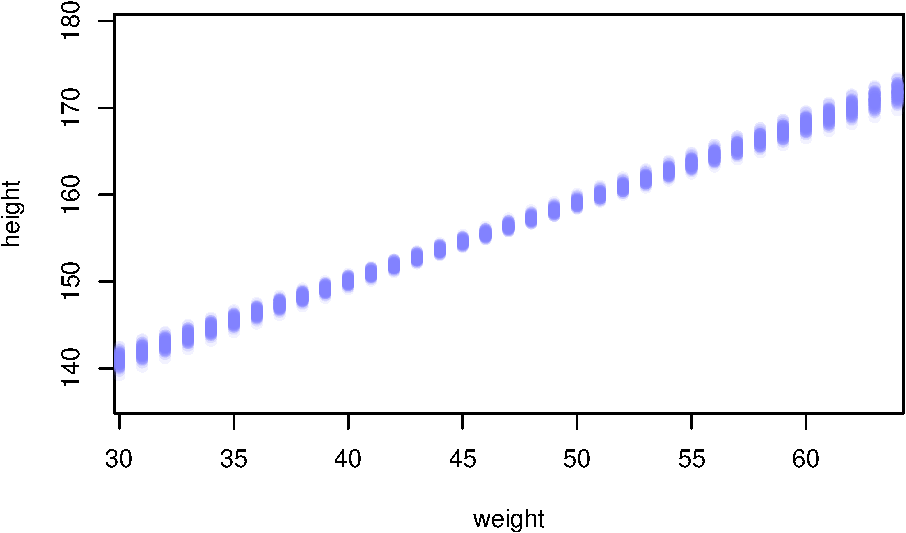
\includegraphics[keepaspectratio]{bookdown-demo_files/figure-latex/unnamed-chunk-29-1.pdf}}

The lighter and wider shaded region is where the model expects to find 89\%
of the heights of a person with a certain weight.

This part is \textbf{sometimes a bit desillusioning} when seen for the first time:
Draw a horizontal line at 150 cm and see how many weights (according to
the individual prediction) are compatible with this height. Weights
from 30 to 50 kg are compatible with this height according to the
89\% prediction interval:

\pandocbounded{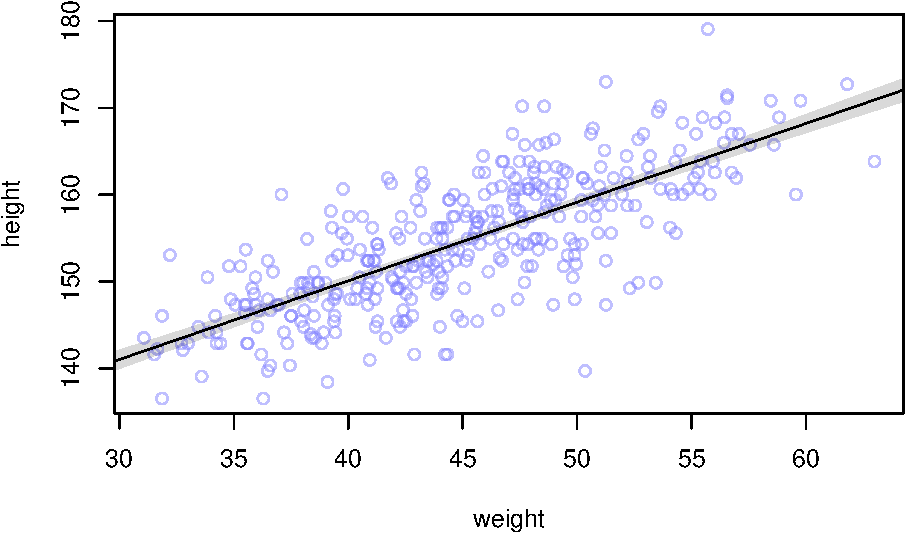
\includegraphics[keepaspectratio]{bookdown-demo_files/figure-latex/unnamed-chunk-30-1.pdf}}

The higher the credibility, the wider the interval,
the wider the range of compatible weights.
In our example, more than 60\% of the weight-range are
plausible to predict a height of 150 cm.

\begin{Shaded}
\begin{Highlighting}[]
\NormalTok{(}\DecValTok{50} \SpecialCharTok{{-}} \DecValTok{30}\NormalTok{) }\SpecialCharTok{/}\NormalTok{ (}\FunctionTok{range}\NormalTok{(d2}\SpecialCharTok{$}\NormalTok{weight)[}\DecValTok{2}\NormalTok{] }\SpecialCharTok{{-}} \FunctionTok{range}\NormalTok{(d2}\SpecialCharTok{$}\NormalTok{weight)[}\DecValTok{1}\NormalTok{])}
\end{Highlighting}
\end{Shaded}

\begin{verbatim}
## [1] 0.6265362
\end{verbatim}

On the other hand: We did not model the relationship this way.
We modeled \textbf{height depending on weight} and not the other way around.
In the next chapter, we will regress weight on height (yes, this is the correct order)
and see what changes.

\subsection{Summary}\label{summary}

\begin{itemize}
\tightlist
\item
  We have added a covariate (weight) to the simple mean model to predict height.
\item
  We have centered the weight variable.
\item
  We have defined and refined priors for the intercept and slope.
\item
  We have estimated the posterior distribution of the parameters using quadratic approximation with \texttt{quap}.
\item
  We have visualized the result.
\item
  We have created credible bands for mean and individual predictions.
\end{itemize}

\section{Simple Linear Regression in the Frequentist Framework}\label{simple-linear-regression-in-the-frequentist-framework}

We will now do the same analysis in the frequentist framework while introducing
some foundational theory along the way.
I recommend reading the first couple of chapters from \href{https://www.routledge.com/Understanding-Regression-Analysis-A-Conditional-Distribution-Approach/Westfall-Arias/p/book/9780367493516?srsltid=AfmBOore3O_Ciecl0TTkr9AjPIY1d6OmbQa7o7IAdKpTSkD8s9HkwzD4}{Westfall}.

\subsection{Model definition}\label{model-definition-1}

Our linear model is defined as:

\[ h_i = \beta_0 + \beta_1 x_i + \varepsilon_i \]

where

\begin{itemize}
\tightlist
\item
  \(\varepsilon_i\) is the error term with \(\varepsilon_i \sim N(0, \sigma), \forall i\)
\item
  \(\beta_0\) is the unknown but fixed intercept
\item
  \(\beta_1\) is the unknown but fixed slope
\end{itemize}

\subsubsection{\texorpdfstring{Model Assumptions of the Classical Regression Model (\href{https://www.routledge.com/Understanding-Regression-Analysis-A-Conditional-Distribution-Approach/Westfall-Arias/p/book/9780367493516?srsltid=AfmBOore3O_Ciecl0TTkr9AjPIY1d6OmbQa7o7IAdKpTSkD8s9HkwzD4}{Westfall}, 1.7):}{Model Assumptions of the Classical Regression Model (Westfall, 1.7):}}\label{_model_assumptions}

The first and \textbf{most important assumption} is that the data are produced\\
probabilistically, which is specifically stated as
\[ Y|X = x \sim p(y|x)\]

What does this mean?

\begin{itemize}
\tightlist
\item
  \(Y|X = x\) is the random variable Y \textbf{conditional} on X being equal to x, i.e.~the
  distribution of \(Y\) if we know the value of \(X\) (in our example the weight in kg).
  \href{https://blogs.sas.com/content/iml/files/2015/09/GLM_normal_identity.png}{This} is a nice image of what is meant here.
\item
  \(p(y|x)\) is the distribution of potentially observable \(Y\) given \(X = x\).
  In our case above this was the normal distribution with mean \(\mu_i\) and variance \(\sigma\).
\end{itemize}

You can play with \href{https://psychmeth.shinyapps.io/Regression-NVFehler/}{this shiny app} to improve your understanding.
It offers the option ``Bedingte Verteilung anzeigen''.

One always thinks about the so-called
\href{https://en.wikipedia.org/wiki/Data_generating_process}{data generating process}
(\href{https://www.routledge.com/Understanding-Regression-Analysis-A-Conditional-Distribution-Approach/Westfall-Arias/p/book/9780367493516?srsltid=AfmBOore3O_Ciecl0TTkr9AjPIY1d6OmbQa7o7IAdKpTSkD8s9HkwzD4}{Westfall}, 1.2).
How did the data come about? There is a process behind it and this process
is attempted to be modeled.

\textbf{Further assumptions}:

\begin{itemize}
\item
  \textbf{Correct functional specification}: The conditional mean function \(f(x) = \mathbb{E}(Y|X=x)\).
  In the case of the linear model, the assumption is \(\mathbb{E}(Y|X=x) = \alpha + \beta x\).
  The \textbf{expectation} of \(Y\) (height) depends linearly on \(x\) (weight).
  This assumption is violated when the true relationship is not linear or the
  data at least suggest that it is not linear, like \href{https://www.alexanderdemos.org/Class5_files/figure-html/unnamed-chunk-2-1.png}{here}.
\item
  \textbf{The errors are homoscedastic} (constant variance \(\sigma\)). This means the
  variances of all conditional distributions \(p(y|x)\) are constant (\(=\sigma^2\)).
  This assumption is violated if points are \href{https://www.investopedia.com/thmb/n9S9lWMv6X9-sKC2DtAOtUTPSik=/1500x0/filters:no_upscale():max_bytes(150000):strip_icc():format(webp)/Heteroskedasticity22-ce5acc2acef6494d91935588b0599579.png}{spreading out more and more
  around the regression line},
  indicating that the errors are getting larger.
\item
  \textbf{Normality}. For the classical linear regression model all the conditional
  distributions \(p(y|x)\) are normal distributions. It could well be, that
  the errors are not nicely normally distributed around the regression line,
  for instance if we have a lot of outliers upwards and the distribution
  is skewed, like \href{https://www.bookdown.org/rwnahhas/RMPH/mlr-normality.html}{here}.
\item
  The \textbf{errors are independent} of each other.
  The potentially observable \(\varepsilon_i = Y_i - f(\mathbf{x_i}, \mathbf{\beta})\)
  is uncorrelated with \(\varepsilon_j = Y_j - f(\mathbf{x_j}, \mathbf{\beta})\) for
  \(i \neq j\). This assumption is violated if the errors are correlated,
  here is an example: The true data comes from a sine curve and we estimate a
  linear model (green), which does not fit the data well (left plot).
  The residuals plot shows clear patterns (right plot) and indicates
  that the errors are correlated. Specifically, the errors around \(x=2\) and \(x=4\)
  are negatively correlated (see \hyperref[exercise6_simpl_lin_reg]{exercise 6}).
\end{itemize}

\begin{verbatim}
## 
## Attaching package: 'patchwork'
\end{verbatim}

\begin{verbatim}
## The following object is masked from 'package:MASS':
## 
##     area
\end{verbatim}

\pandocbounded{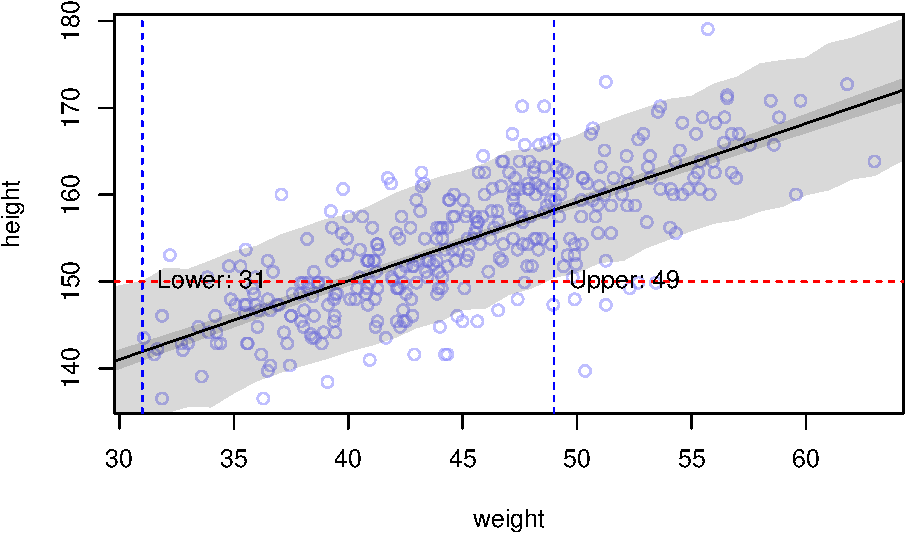
\includegraphics[keepaspectratio]{bookdown-demo_files/figure-latex/unnamed-chunk-32-1.pdf}}

In the case above, the errors are \textbf{not conditionally independent}.
If we condition on \(X=2\) and \(X=4.5\), the errors are correlated (\(r \sim -0.3\)),
which they should not be.

These assumptions become clearer as we go along and should be checked
for every model we fit. They are not connected, they can all be true or false.
The question is not ``Are the assumptions met?'' since they never are exactly met.
The question is \textbf{how} ``badly'' the assumptions are violated?

Remember, \textbf{all models are wrong, but some are useful}.

In full, the classical linear regression model can be written as:

\[ Y_i|X_i = x_i \sim_{independent} N(\beta_0 + \beta_1 x_{i1} + \dots \beta_k x_{ik},\sigma^2)\]
for \(i = 1, \dots, n\).

\subsection{Fit the model}\label{fit_model_simple_lin_reg_classic}

Again, we fit the model using the least squares method. For a neat animated explanation,
visit \href{https://www.youtube.com/watch?v=jEEJNz0RK4Q&ab_channel=COCCmath}{this video}.
There are literally hundreds of videos on the topic. Choose wisely. Not all are good.
If in doubt, use our recommended books as reading materials. This is the most reliable source.
A hint along the way: Be very sceptical if you ask GPT about information,
although for this special case one has a good chance of getting a good answer due to
the vast amount of training data.

One has to minimize the sum of squared differences between the true heights and
the model-predicted heights in order to find \(\beta_0\) and \(\beta_1\).

\[ SSE(\beta_0, \beta_1) = \sum_{i=1}^n (y_i - (\beta_0 + \beta_1 x_i))^2 \]

We omit the technical details (set derivative to zero and solve the system) and give the results for \(\beta_0\) and \(\beta_1\):

\[
\hat{\beta_0} = \bar{y} - (\hat{\beta_1} \bar{x}),
\]
\[
\hat{\beta_1} = \frac{\sum_{i=1}^n (x_i - \bar{x})(y_i - \bar{y})}{\sum_{i=1}^n (x_i - \bar{x})^2} =
 \frac{s_{x,y}}{s_x^2} = r_{xy} \frac{s_y}{s_x}.
\]

where:

\begin{itemize}
\tightlist
\item
  \(r_{xy}\) is the \href{https://en.wikipedia.org/wiki/Pearson_correlation_coefficient}{sample correlation coefficient} between \(x\) and \(y\)
\item
  \(s_x\) and \(s_y\) are the \href{https://en.wikipedia.org/wiki/Standard_deviation}{uncorrected sample standard deviations} of \(x\) and \(y\)
\item
  \(s_x^2\) and \(s_{xy}\) are the \href{https://en.wikipedia.org/wiki/Variance}{sample variance} and \href{https://en.wikipedia.org/wiki/Covariance}{sample covariance}, respectively
\end{itemize}

Interpretation of \(\hat{\beta}_0\) and \(\hat{\beta}_1\): see \hyperref[exercise3_simpl_lin_reg]{exercise 3}.

Let's \textbf{use R again to solve the problem}:

\begin{Shaded}
\begin{Highlighting}[]
\FunctionTok{library}\NormalTok{(rethinking)}
\FunctionTok{data}\NormalTok{(Howell1)}
\NormalTok{d }\OtherTok{\textless{}{-}}\NormalTok{ Howell1}
\NormalTok{d2 }\OtherTok{\textless{}{-}}\NormalTok{ d[d}\SpecialCharTok{$}\NormalTok{age }\SpecialCharTok{\textgreater{}=} \DecValTok{18}\NormalTok{, ]}
\NormalTok{mod }\OtherTok{\textless{}{-}} \FunctionTok{lm}\NormalTok{(height }\SpecialCharTok{\textasciitilde{}}\NormalTok{ weight, }\AttributeTok{data =}\NormalTok{ d2)}
\FunctionTok{summary}\NormalTok{(mod)}
\end{Highlighting}
\end{Shaded}

\begin{verbatim}
## 
## Call:
## lm(formula = height ~ weight, data = d2)
## 
## Residuals:
##      Min       1Q   Median       3Q      Max 
## -19.7464  -2.8835   0.0222   3.1424  14.7744 
## 
## Coefficients:
##              Estimate Std. Error t value Pr(>|t|)    
## (Intercept) 113.87939    1.91107   59.59   <2e-16 ***
## weight        0.90503    0.04205   21.52   <2e-16 ***
## ---
## Signif. codes:  0 '***' 0.001 '**' 0.01 '*' 0.05 '.' 0.1 ' ' 1
## 
## Residual standard error: 5.086 on 350 degrees of freedom
## Multiple R-squared:  0.5696, Adjusted R-squared:  0.5684 
## F-statistic: 463.3 on 1 and 350 DF,  p-value: < 2.2e-16
\end{verbatim}

\textbf{Interpretation of R-output}:

\begin{itemize}
\tightlist
\item
  \texttt{Call}: The model that was fitted.
\item
  \texttt{Residuals}: \(r_i = height_i - \widehat{height}_i\).
  Differences between true heights and model-predicted heights.
\item
  \texttt{Coefficients}: Estimated for \(\beta_0\) and \(\beta_1\). We call them \(\hat{\beta}_0\) and \(\hat{\beta}_1\).

  \begin{itemize}
  \tightlist
  \item
    \texttt{Estimate}: The (least squares) estimated value of the coefficient.
  \item
    \texttt{Std.\ Error}: The standard error of the estimate.
  \item
    \texttt{t\ value}: The value of the \(t\)-statistic for the (Wald-) hypothesis test
    \(H_0: \beta_i = 0\).
  \item
    \texttt{Pr(\textgreater{}\textbar{}t\textbar{})}: The \(p\)-value of the hypothesis test.
  \end{itemize}
\item
  \texttt{Residual\ standard\ error}: The estimate of \(\sigma\)
  which is also a model parameter (as in the Bayesian framework).
\item
  \texttt{Multiple\ R-squared}: The proportion of the variance explained by the
  model (we will explain this below).
\item
  \texttt{Adjusted\ R-squared}: A corrected version of the \(R^2\) which takes into account
  the number of predictors in the model.
\item
  \texttt{F-statistic}: The value of the \(F\)-statistic for the hypothesis test:
  \(H_0: \beta_1 = \beta_2 = \dots = \beta_k = 0\). Note, the alternative
  hypotheses to this test is that \emph{any} of the \(\beta_i\) is not zero. If that is
  the case, the model explains more than the mean model with just \(\beta_0\).
\end{itemize}

We could also \textbf{solve the least squares problem graphically}: We want to find the
values of \(\beta_0\) and \(\beta_1\) that minimize the sum of squared differences
which can be plotted as 3D function. Since the function is a sum of squared terms,
we should expected a paraboloid form.
All we have to do is to ask R which of
the coordinates (\(\beta_0\), \(\beta_1\)) minimizes the sum of squared errors. The result confirmes
the results from the \texttt{lm} function. The dot in red marks the spot
(Code is in the \href{https://github.com/jdegenfellner/Script_QM2_ZHAW}{git repository}):

\textbf{---COMPILE CODE AT DEOPLOYMENT (takes a bit)---}

\subsection{Confidence Intervals of coefficients (frequentist)}\label{confidence_intervals_frequentist}

You can get CI's conveniently with the \texttt{confint} function:

\begin{Shaded}
\begin{Highlighting}[]
\FunctionTok{confint}\NormalTok{(mod, }\AttributeTok{level =} \FloatTok{0.96}\NormalTok{)}
\end{Highlighting}
\end{Shaded}

\begin{verbatim}
##                    2 %        98 %
## (Intercept) 109.939864 117.8189232
## weight        0.818351   0.9917072
\end{verbatim}

Remember, these are frequenetist confidence intervals.

\textbf{If one repeats the experiment
many times, the true but unknown value of the parameter will
be in the interval in 96\% of the cases}

We can also use the simple \href{https://en.wikipedia.org/wiki/Bootstrapping_(statistics)}{bootstrap}.
The advantage of this tequique is that we can basically always use it,
no matter how compliated the estimator is. We do not need formulae.
We simply

\begin{itemize}
\tightlist
\item
  create 1000 bootstrap samples,
\item
  fit the model,
\item
  store the coefficients.
\item
  The 2\% and 98\% quantiles of the coefficients constitute the 96\% bootstrap confidence interval.
\end{itemize}

\begin{Shaded}
\begin{Highlighting}[]
\FunctionTok{set.seed}\NormalTok{(}\DecValTok{123}\NormalTok{)}
\NormalTok{n }\OtherTok{\textless{}{-}} \FunctionTok{nrow}\NormalTok{(d2)}
\NormalTok{B }\OtherTok{\textless{}{-}} \DecValTok{1000}
\NormalTok{boot\_coefs }\OtherTok{\textless{}{-}} \FunctionTok{matrix}\NormalTok{(}\ConstantTok{NA}\NormalTok{, }\AttributeTok{nrow =}\NormalTok{ B, }\AttributeTok{ncol =} \DecValTok{2}\NormalTok{)}
\ControlFlowTok{for}\NormalTok{ (i }\ControlFlowTok{in} \DecValTok{1}\SpecialCharTok{:}\NormalTok{B) \{}
\NormalTok{  boot\_idx }\OtherTok{\textless{}{-}} \FunctionTok{sample}\NormalTok{(}\DecValTok{1}\SpecialCharTok{:}\NormalTok{n, }\AttributeTok{replace =} \ConstantTok{TRUE}\NormalTok{)}
\NormalTok{  boot\_mod }\OtherTok{\textless{}{-}} \FunctionTok{lm}\NormalTok{(height }\SpecialCharTok{\textasciitilde{}}\NormalTok{ weight, }\AttributeTok{data =}\NormalTok{ d2[boot\_idx, ])}
\NormalTok{  boot\_coefs[i, ] }\OtherTok{\textless{}{-}} \FunctionTok{coef}\NormalTok{(boot\_mod)}
\NormalTok{\}}
\CommentTok{\#head(boot\_coefs)}
\FunctionTok{quantile}\NormalTok{(boot\_coefs, }\FunctionTok{c}\NormalTok{(}\FloatTok{0.02}\NormalTok{, }\FloatTok{0.98}\NormalTok{), }\AttributeTok{na.rm =} \ConstantTok{TRUE}\NormalTok{)}
\end{Highlighting}
\end{Shaded}

\begin{verbatim}
##          2%         98% 
##   0.8343242 117.0319290
\end{verbatim}

\begin{Shaded}
\begin{Highlighting}[]
\FunctionTok{t}\NormalTok{(}\FunctionTok{apply}\NormalTok{(boot\_coefs, }\DecValTok{2}\NormalTok{, quantile, }\FunctionTok{c}\NormalTok{(}\FloatTok{0.02}\NormalTok{, }\FloatTok{0.98}\NormalTok{)))}
\end{Highlighting}
\end{Shaded}

\begin{verbatim}
##               2%         98%
## [1,] 110.1862455 117.4516455
## [2,]   0.8229982   0.9859997
\end{verbatim}

The CIs are quite similar to the ones from the \texttt{confint} function.

In the Bayesian setting, we used the centered weight variable. Let's to this here too for
comparison and use 89\% coverage probability.

\begin{Shaded}
\begin{Highlighting}[]
\NormalTok{d2}\SpecialCharTok{$}\NormalTok{weight\_centered }\OtherTok{\textless{}{-}}\NormalTok{ d2}\SpecialCharTok{$}\NormalTok{weight }\SpecialCharTok{{-}} \FunctionTok{mean}\NormalTok{(d2}\SpecialCharTok{$}\NormalTok{weight)}
\NormalTok{mod\_centered }\OtherTok{\textless{}{-}} \FunctionTok{lm}\NormalTok{(height }\SpecialCharTok{\textasciitilde{}}\NormalTok{ weight\_centered, }\AttributeTok{data =}\NormalTok{ d2)}
\CommentTok{\#summary(mod\_centered)}
\FunctionTok{confint}\NormalTok{(mod\_centered, }\AttributeTok{level =} \FloatTok{0.89}\NormalTok{)}
\end{Highlighting}
\end{Shaded}

\begin{verbatim}
##                      5.5 %      94.5 %
## (Intercept)     154.162715 155.0314698
## weight_centered   0.837658   0.9724002
\end{verbatim}

Compare with \texttt{precis} from the Bayesian model:

\begin{verbatim}
##              mean         sd       5.5%       94.5%
## a     154.5972131 0.27033041 154.165173 155.0292533
## b       0.9050133 0.04192753   0.838005   0.9720216
## sigma   5.0718667 0.19115317   4.766367   5.3773663
\end{verbatim}

We are glad to see that both analyses align really nicely.

\subsection{ANOVA (Analysis of Variance)}\label{analysis_of_variance}

A non-obvious and very useful finding is that the total variability (SST)
in the data (our heights) can be
\textbf{decomposed} (or \href{https://en.wiktionary.org/wiki/analysis}{analysed})
into two parts:

\begin{itemize}
\tightlist
\item
  The variability explained by the model (the regression line): SSR
\item
  The variability not explained by the model (the residuals): SSE
\end{itemize}

\[ \text{Sum of Squares in Total} = \text{Sum of Squares from Regression} + \text{Sum of Squared Errors} \]

\[ SST = SSR + SSE \]

\[ \sum_{i=1}^{n} (y_i - \bar{y})^2 = \sum_{i=1}^{n} (\hat{y}_i - \bar{y})^2 + \sum_{i=1}^{n} (y_i - \hat{y}_i)^2 \]

If you are interested in the details, check out \href{https://en.wikipedia.org/wiki/Explained_sum_of_squares\#Partitioning_in_the_general_ordinary_least_squares_model}{this}.

\href{https://www.youtube.com/watch?v=NxRTs7sXKAQ&ab_channel=365DataScience}{This video}
explains the concept nicely.

Let's visualize our regression result:

\begin{verbatim}
## `geom_smooth()` using formula = 'y ~ x'
\end{verbatim}

\pandocbounded{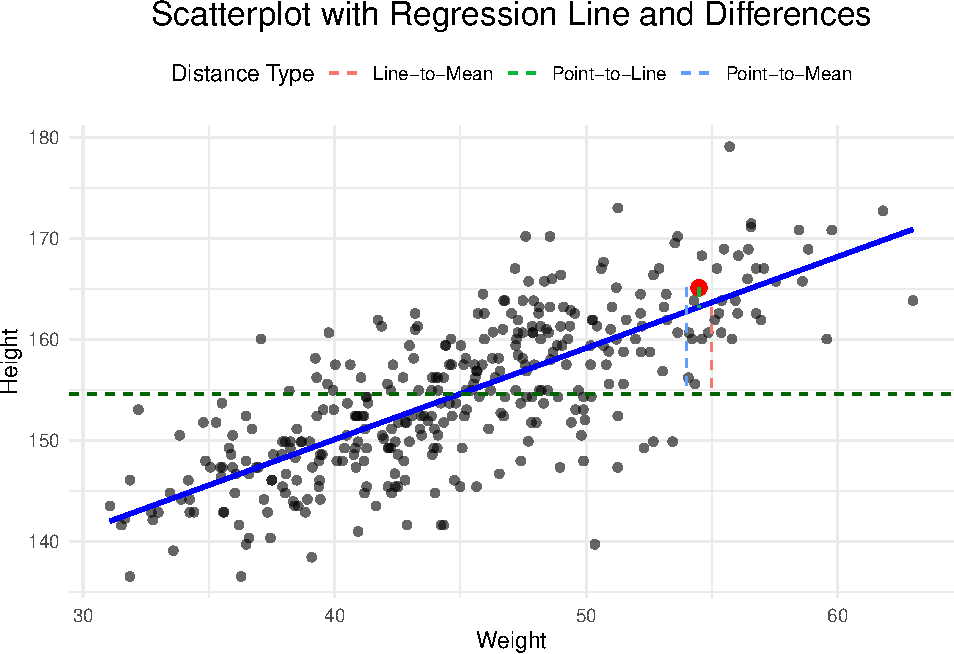
\includegraphics[keepaspectratio]{bookdown-demo_files/figure-latex/unnamed-chunk-39-1.pdf}}

The blue dotted line is the distance from
the mean to the point (total variance), the red dotted line is the distance from
the mean to the regression line (explained variance) and the green dotted line
is the distance from the regression line to the point (unexplained variance).
We see that it adds up. I find this fact quite fascinating.
One finds additivity by considering not determinisic values, but variances.
Thank you \href{https://en.wikipedia.org/wiki/Analysis_of_variance\#:~:text=ANOVA\%20was\%20developed\%20by\%20the,to\%20different\%20sources\%20of\%20variation.}{Ronald Fisher}.

\subsection{\texorpdfstring{\(R^2\) - Coefficient of Determination}{R\^{}2 - Coefficient of Determination}}\label{r2---coefficient-of-determination}

\href{https://en.wikipedia.org/wiki/Coefficient_of_determination}{\(R^2\)}
is the \textbf{amount of variance explained by the model}.
You can also read \href{https://www.routledge.com/Understanding-Regression-Analysis-A-Conditional-Distribution-Approach/Westfall-Arias/p/book/9780367493516?srsltid=AfmBOore3O_Ciecl0TTkr9AjPIY1d6OmbQa7o7IAdKpTSkD8s9HkwzD4}{Westfall} 8.1.

As you can see
\hyperref[analysis_of_variance]{above}, the total variance (SST) of our outcome (height)
can be decomposed into two parts: the variance explained by the model (SSR)
and the variance not explained by the model (SSE).

Maybe the most intuitive definition of \(R^2\) is:

\[ R^2 = \frac{SSR}{SST} = \frac{SST - SSE}{SST} = 1 - \frac{SSE}{SST}\]

The value is between 0 and 1. The higher the value, the more variance is explained.
But be cautious. Depending on the context, a really high \(R^2\) is not
necessarily a good thing. With the data we are working with,
it could easily hint towards an error. If we are near 1,
all points in the simple linear regression model are on the line.
If we are near 0, the model does not explain much of the variance
and we would see ``noise with no slope'' in the scatterplot (\hyperref[exercise4_simpl_lin_reg]{exercise 4}).
The normal \(R^2\) can be found in the R output under \texttt{Multiple\ R-squared}.

If you add a lot of variables to your regression model, you can get an
\(R^2\) of 1. The \(R^2\) will never decrease when adding more variables.
We will verify this when we have more than 2 explanatory variables.
As a non-formal explanation for this: In the Sum of Squares Errors (SSE),
if you add more covariates (\(\beta_2, \beta_3\)), you have more freedom
to choose values that minimize the number that will be squared. Simple regression
is just a special case of multiple (more than one predictor) regression with \(\beta_2=\beta_3=\dots=0\).
Hence, you will definitely not be worse off with regards to SSE when using more covariates.
A smaller SSE implies a larger SSR (sum constraint; SST remains constant) and hence a larger \(R^2\).
If you have as many explanatory variables as data points, you can get an \(R^2\) of 1. This is
\href{https://en.wikipedia.org/wiki/Overfitting}{overfitting} at its ``best'' (which we want to avoid).
You would just get a value for each data point by setting all other \(\beta_i\) to zero and
\(\beta_i = \frac{y_i}{x_i}\).
Since we want to find the unterlying process, we want to avoid this.

Although not perfect, one way to mitigate the influence of ``too many'' variables
on \(R^2\) is to use the adjusted \(R^2\), which an also be found in the R output (\texttt{Adjusted\ R-squared}).

\subsubsection{\texorpdfstring{Seperating property of regression due to \(R^2\):}{Seperating property of regression due to R\^{}2:}}\label{seperating_property}

\href{https://www.routledge.com/Understanding-Regression-Analysis-A-Conditional-Distribution-Approach/Westfall-Arias/p/book/9780367493516?srsltid=AfmBOore3O_Ciecl0TTkr9AjPIY1d6OmbQa7o7IAdKpTSkD8s9HkwzD4}{Peter Westfall}
explains (in Figure 8.1 of the book) how \(R^2\) influences the separation of distributions in our simple regression model.

In our regression of \emph{height on weight} (the order is correct, that's how you say it),
the \(R^2\) is \(0.5696\). The following plot shows how ``well'' (i.e.~precise) one can predict
height if we use the 10\% and 90\% quantile of the weights (x\_low and x\_high).
In both, you see the conditional distribution of height given the weight \(X = x_{low}\) or \(X = x_{high}\).
Scenario 1 is the original model, scenario 2 is the same data with added noise (in Y-direction),
which reduces \(R^2\) to \(0.13\), much lower. In the right plot, the distributions have a large
overlap and it is hard to distinguish between weights when seeing the height.
With a very low \(R^2\), the height prediction does not really change and we could just as well
use the mean model.

\pandocbounded{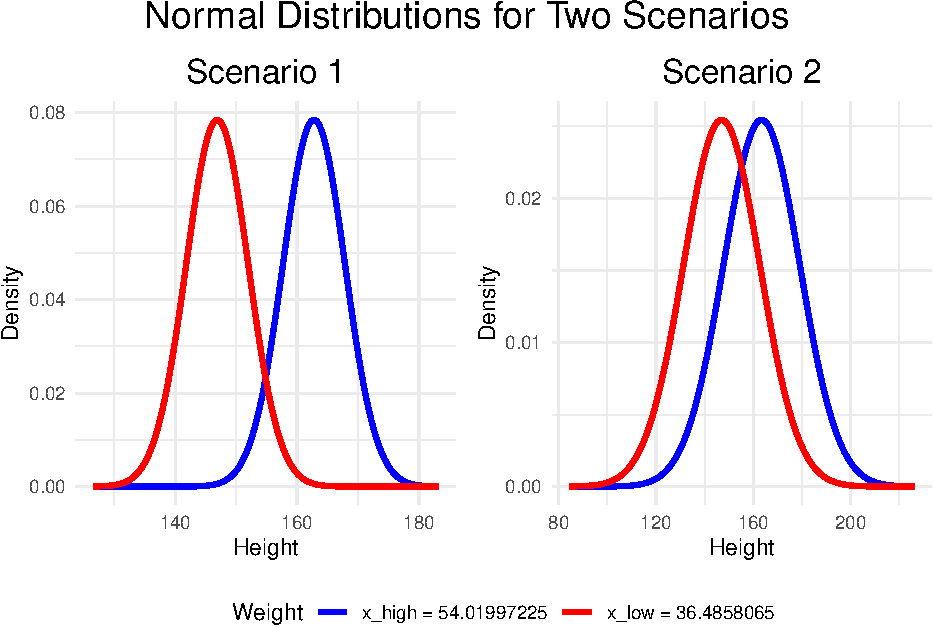
\includegraphics[keepaspectratio]{bookdown-demo_files/figure-latex/unnamed-chunk-40-1.pdf}}

In the left plot, given \(X = x_{low}\) gives a a rather strongly shifted normal distribution of
potentially observable heights for this weight compared to \(X=x_{high}\).
We would have a lower missclassification error when trying to distinguish heights
of very light and very heavy people in the sample just by seeing the height.
You can think of an even more extreme separation of these distributions,
which would happen, when \(R^2\) is very high or the true slope is much higher.

See also \hyperref[exercise5_simpl_lin_reg]{exercise 5}.

An interesting way to look at \(R^2\) is the following:
Given, that one person is in the 90\% quantile of the weight,
the other is in the 10\% quantile. What is the probability that the
height of the person in the 90\% quantile is higher than the height of the other person?
We could calculate this relatively easy using theorems about additivity of normal distributions.
Since we are all about application, we simulate this:

\begin{Shaded}
\begin{Highlighting}[]
\FunctionTok{library}\NormalTok{(rethinking)}
\FunctionTok{data}\NormalTok{(Howell1)}
\NormalTok{d }\OtherTok{\textless{}{-}}\NormalTok{ Howell1}
\NormalTok{d2 }\OtherTok{\textless{}{-}}\NormalTok{ d[d}\SpecialCharTok{$}\NormalTok{age }\SpecialCharTok{\textgreater{}=} \DecValTok{18}\NormalTok{, ]}
\CommentTok{\# Simulate heights for the two quantiles}
\NormalTok{n\_sims }\OtherTok{\textless{}{-}} \DecValTok{10000}
\FunctionTok{set.seed}\NormalTok{(}\DecValTok{123}\NormalTok{)}
\NormalTok{mod }\OtherTok{\textless{}{-}} \FunctionTok{lm}\NormalTok{(height }\SpecialCharTok{\textasciitilde{}}\NormalTok{ weight, }\AttributeTok{data =}\NormalTok{ d2)}
\FunctionTok{summary}\NormalTok{(mod)}\SpecialCharTok{$}\NormalTok{r.squared}
\end{Highlighting}
\end{Shaded}

\begin{verbatim}
## [1] 0.5696444
\end{verbatim}

\begin{Shaded}
\begin{Highlighting}[]
\NormalTok{x\_low\_high }\OtherTok{\textless{}{-}} \FunctionTok{quantile}\NormalTok{(d2}\SpecialCharTok{$}\NormalTok{weight, }\AttributeTok{probs =} \FunctionTok{c}\NormalTok{(}\FloatTok{0.1}\NormalTok{, }\FloatTok{0.9}\NormalTok{))}
\NormalTok{x\_low\_high}
\end{Highlighting}
\end{Shaded}

\begin{verbatim}
##      10%      90% 
## 36.48581 54.01997
\end{verbatim}

\begin{Shaded}
\begin{Highlighting}[]
\NormalTok{mean1 }\OtherTok{\textless{}{-}} \FloatTok{113.8793936} \SpecialCharTok{+} \FloatTok{0.9050291} \SpecialCharTok{*}\NormalTok{ x\_low\_high[}\DecValTok{1}\NormalTok{]}
\NormalTok{mean2 }\OtherTok{\textless{}{-}} \FloatTok{113.8793936} \SpecialCharTok{+} \FloatTok{0.9050291} \SpecialCharTok{*}\NormalTok{ x\_low\_high[}\DecValTok{2}\NormalTok{]}
\NormalTok{sd }\OtherTok{\textless{}{-}} \FloatTok{5.086}  \CommentTok{\# Standard deviation for both distributions}
\NormalTok{simulated\_heights }\OtherTok{\textless{}{-}} \FunctionTok{tibble}\NormalTok{(}
  \CommentTok{\# conditional normal distribution according to the model}
  \AttributeTok{x\_low =} \FunctionTok{rnorm}\NormalTok{(n\_sims, }\AttributeTok{mean =}\NormalTok{ mean1, }\AttributeTok{sd =}\NormalTok{ sd),}
  \AttributeTok{x\_high =} \FunctionTok{rnorm}\NormalTok{(n\_sims, }\AttributeTok{mean =}\NormalTok{  mean2, }\AttributeTok{sd =}\NormalTok{ sd)}
\NormalTok{)}

\CommentTok{\# Calculate the probability that the height of the person in the 90\% quantile is higher}
\CommentTok{\# than the height of the person in the 10\% quantile}
\NormalTok{simulated\_heights }\SpecialCharTok{\%\textgreater{}\%}
  \FunctionTok{mutate}\NormalTok{(}\AttributeTok{higher\_height =}\NormalTok{ x\_high }\SpecialCharTok{\textgreater{}}\NormalTok{ x\_low) }\SpecialCharTok{\%\textgreater{}\%}
\NormalTok{  dplyr}\SpecialCharTok{::}\FunctionTok{summarise}\NormalTok{(}\FunctionTok{mean}\NormalTok{(higher\_height))}
\end{Highlighting}
\end{Shaded}

\begin{verbatim}
## # A tibble: 1 x 1
##   `mean(higher_height)`
##                   <dbl>
## 1                 0.987
\end{verbatim}

In other words, we can be almost sure, that a person in the 90\% quantile of the weight
is taller than a person in the 10\% quantile of the weight given this data set.
See also \hyperref[exercise11_simpl_lin_r]{exercise 11}.

\subsection{Check regression assumptions}\label{check-regression-assumptions}

Everytime we fit a model, we should check the assumptions \hyperref[_model_assumptions]{above}.
We do this for different reasons (which will become clearer over the course).
The assumptions are independent of each other.
They can all be true or false or some can be true and some false
(\href{https://www.routledge.com/Understanding-Regression-Analysis-A-Conditional-Distribution-Approach/Westfall-Arias/p/book/9780367493516?srsltid=AfmBOore3O_Ciecl0TTkr9AjPIY1d6OmbQa7o7IAdKpTSkD8s9HkwzD4}{Wesftall}, p.21).
Chapter 4 in the book is dedicated to this topic. It is important to know
that the assumptions are usually not met exactly. The question is \emph{how badly} they are violated,
not \emph{if} they are violated.
Furthermore, the asssumptions refer to the data generating process, not the data itself.
Thus, the evaluation of the assumptions should involve subject matter knowledge.

\(p\)-values to evaluate model assumptions are not a good idea. To \href{https://www.tandfonline.com/doi/full/10.1080/00031305.2016.1154108\#d1e949}{quote} the
American Statistical Association (ASA): ``By itself, a \(p\)-value does not provide a good measure
of evidence regarding a model or hypothesis.''
Deicision-tree thinking might not be the best idea for statistical modeling.

We will not use hypothesis tests for assumptions, because

\begin{itemize}
\tightlist
\item
  They are never met exactly. You cannot ``prove'' them.
\item
  With small smaple sizes, the statistical \emph{power} is often low.
\item
  With large sample sizes, the smallest deviation will be ``significant''.
\end{itemize}

We will follow the book (chapter 4, pages 99ff) and use graphical and simulation methods to check the assumptions.
As guidance, we could check the assumptions in the following order:

\begin{itemize}
\tightlist
\item
  Linearity
\item
  Constant variance
\item
  Independence
\item
  Normality
\end{itemize}

\subsubsection{Linearity}\label{linearity}

First, we \textbf{plot the data}, as we did already above. We can add a
a smoothing line to the raw data as well:

\begin{verbatim}
## `geom_smooth()` using formula = 'y ~ x'
\end{verbatim}

\pandocbounded{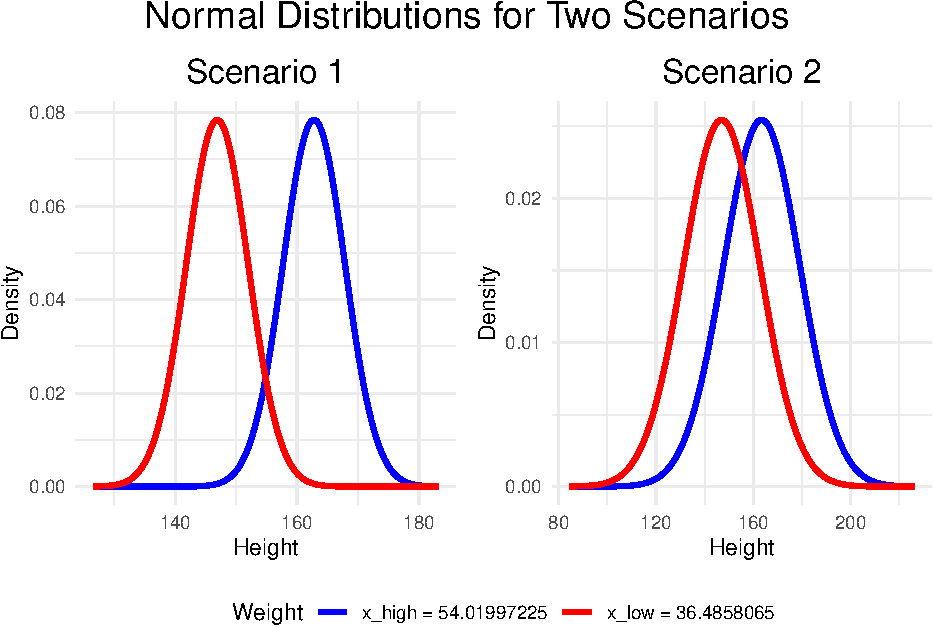
\includegraphics[keepaspectratio]{bookdown-demo_files/figure-latex/unnamed-chunk-42-1.pdf}}

It looks like this relationship is describable in a linear way.
No apparent curvature or patches.
A refined version of the scatterplot of the raw data is The
\textbf{residual scatter plot} (\(x_i, e_i\)):

\begin{verbatim}
## `geom_smooth()` using formula = 'y ~ x'
\end{verbatim}

\pandocbounded{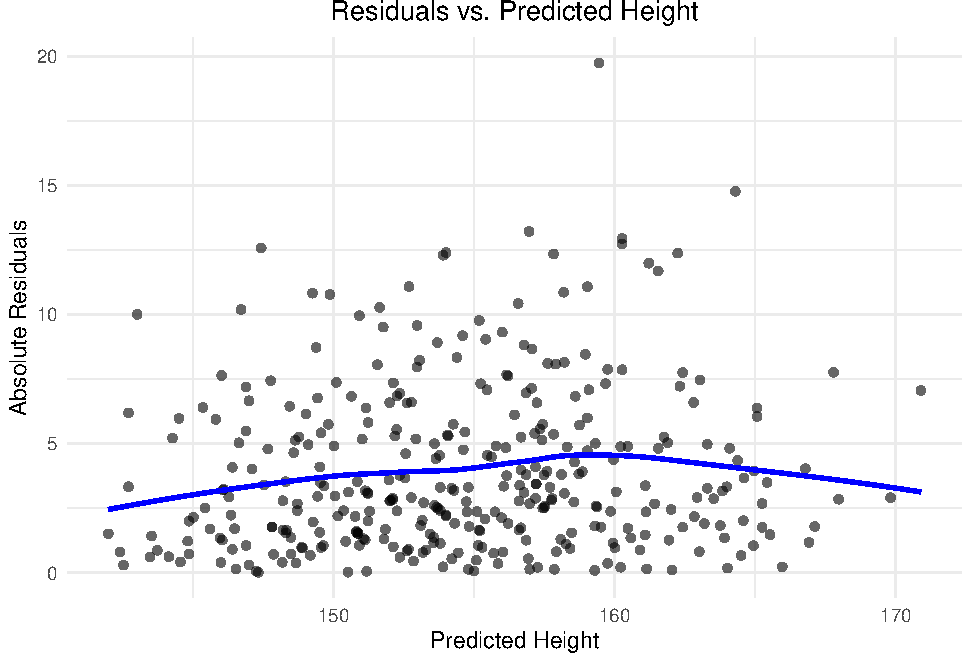
\includegraphics[keepaspectratio]{bookdown-demo_files/figure-latex/unnamed-chunk-43-1.pdf}}

Compared to the scatterplot above, the residuals plot magnifies
possible curvature. The reason is that the range of residuals
is smaller than the range of the heights.

In multiple regression, we will use the (\(\hat{y_i}, e_i\)) plot, which is
identical to the plot above in simple linear regression, but
very helpful in multiple regression.
You get the (\(\hat{y_i}, e_i\)) plot in R with \texttt{plot(mod,\ which\ =\ 1)}.

\subsubsection{Constant variance}\label{constant_variance}

This assumption means that the variance of the residuals is constant.
If it is violated, the spread around a hypothetical regression line is not constant.
We look at the residual scatter plot again:

\pandocbounded{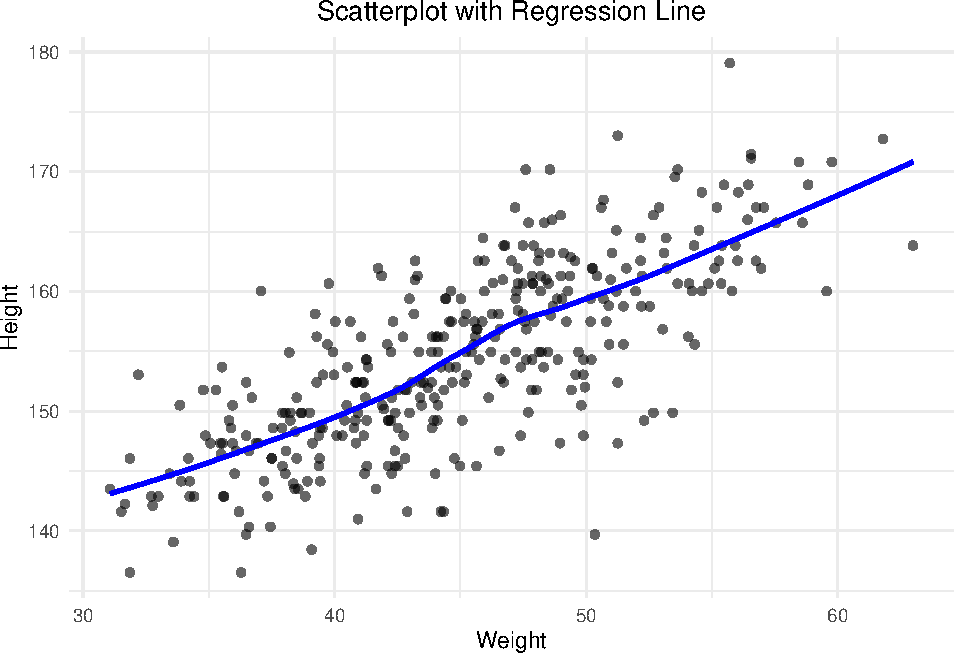
\includegraphics[keepaspectratio]{bookdown-demo_files/figure-latex/unnamed-chunk-44-1.pdf}}

Look for a changes in patterns of vertical variability. Note, that you
often do not have as many data points near the end of the range of the predictor.
Here are some examples of heteroskedasticity:
\href{https://i0.wp.com/statisticsbyjim.com/wp-content/uploads/2017/08/residuals_unfixed.png?resize=576\%2C384}{1},
\href{https://encrypted-tbn0.gstatic.com/images?q=tbn:ANd9GcQPAPMGV5U0Pe0nKnhoZWHJ8KypqVCls6ZQZud84C3KM8SJqOkuMNeJl2oTg-UDuukJRhk&usqp=CAU}{2},
\href{https://i.sstatic.net/R5KIH.png}{3}.
The above looks homoscedastic. If it was heteroskedastic, this is not a problem,
we just have to model it differently (later).

As always, it is a good idea to study the variability of these plots
using simulation (\hyperref[exercise7_simpl_lin_reg]{exercise 7}).

Better for detecting heteroscedasticity is the (\(\hat{y_i}, |e_i|\)) plot
with a smoothing line:

\begin{verbatim}
## 'data.frame':    544 obs. of  4 variables:
##  $ height: num  152 140 137 157 145 ...
##  $ weight: num  47.8 36.5 31.9 53 41.3 ...
##  $ age   : num  63 63 65 41 51 35 32 27 19 54 ...
##  $ male  : int  1 0 0 1 0 1 0 1 0 1 ...
\end{verbatim}

\begin{verbatim}
## `geom_smooth()` using formula = 'y ~ x'
\end{verbatim}

\pandocbounded{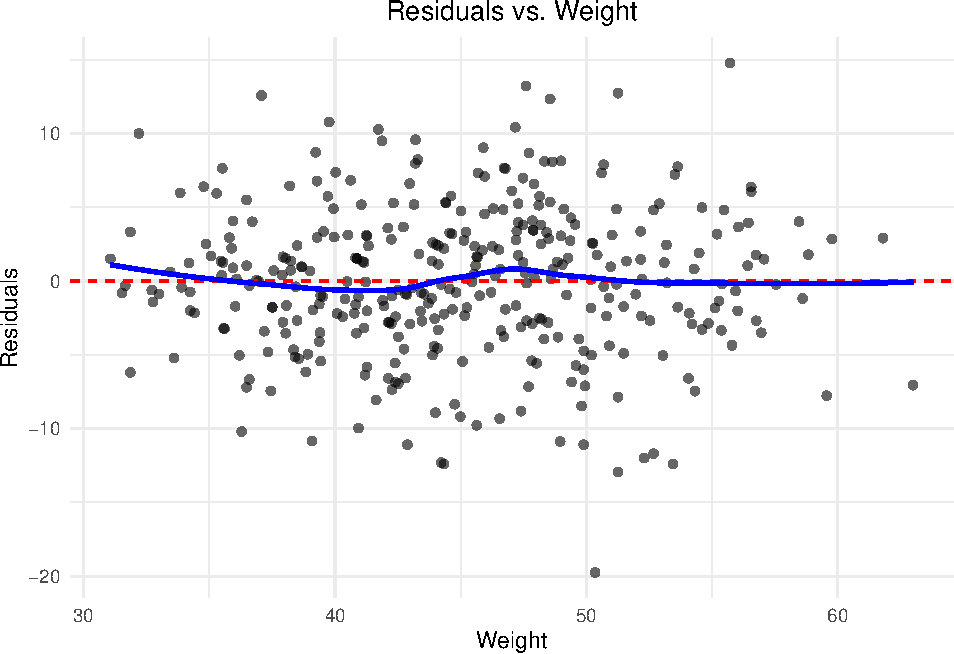
\includegraphics[keepaspectratio]{bookdown-demo_files/figure-latex/unnamed-chunk-45-1.pdf}}

This will probably not be a perfectly horizontal line, since
there are less points at the end of the range of the predictor.
For instance, There are less people with extreme weights in the data set.

\subsubsection{Independence, uncorrelated errors}\label{independence-uncorrelated-errors}

We had a example above, where the errors were correlated.
The sine curve could stem from time series data, where the \(x\)-variable
is the time and the \(y\)-variable is a seasonally changing variable
like temperature (purely hypothetical). In \hyperref[exercise6_simpl_lin_reg]{exercise 6},
the values are autocorrelated: Correlated with previous values of the same variable.
If we would track the body heights of persons over time, we would have
an autocorrelated time series since the height of a person at time \(t\) is
correlated with the height of the same person at time \(t-1\), but a little
less with the height at time \(t-2\) and so on. If I am tall today, it is
very likely that I was tall yesterday.

In our case of the !Kung San data, we do not have autocorrelated data.

But still, we could look at the correlations the residuals with lagged residuals.
A \(lag=1\) means I compare the residuals with the ones right next to me and check if
they are correlated.

\begin{verbatim}
## cor= 0.01858044
\end{verbatim}

\pandocbounded{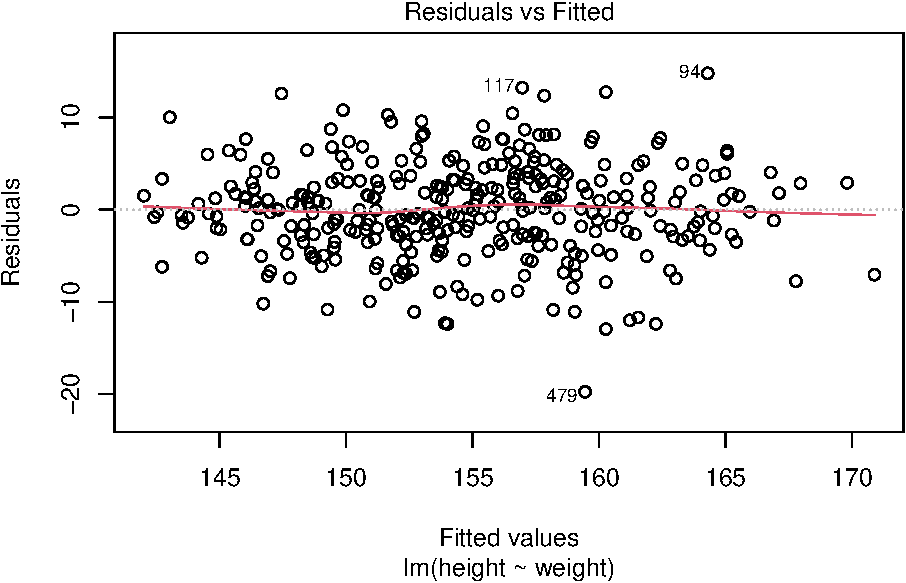
\includegraphics[keepaspectratio]{bookdown-demo_files/figure-latex/unnamed-chunk-46-1.pdf}}

It least with a lag of \(1\), there so no large correlation between the residuals.

\subsubsection{Normality}\label{normality_assumption}

This assumptions states that the conditional distribution \(Y|X=x\)
is a normal distribution. We do not look at the normality of \(Y\) itself,
since it is not a formal requirement, that \(Y\) is normally distributed.
We need to assess the normality of the residuals \[e_i = y_i - \hat{y}_i\]
I like doing this with a \href{https://jdegenfellner.github.io/Script_QM1_ZHAW/descriptive_stats.html\#q-q-plots}{Q-Q plot}
from the R package \texttt{car}:

\begin{verbatim}
## Loading required package: carData
\end{verbatim}

\begin{verbatim}
## 
## Attaching package: 'car'
\end{verbatim}

\begin{verbatim}
## The following object is masked from 'package:dplyr':
## 
##     recode
\end{verbatim}

\begin{verbatim}
## The following object is masked from 'package:purrr':
## 
##     some
\end{verbatim}

\begin{verbatim}
## The following object is masked from 'package:rethinking':
## 
##     logit
\end{verbatim}

\pandocbounded{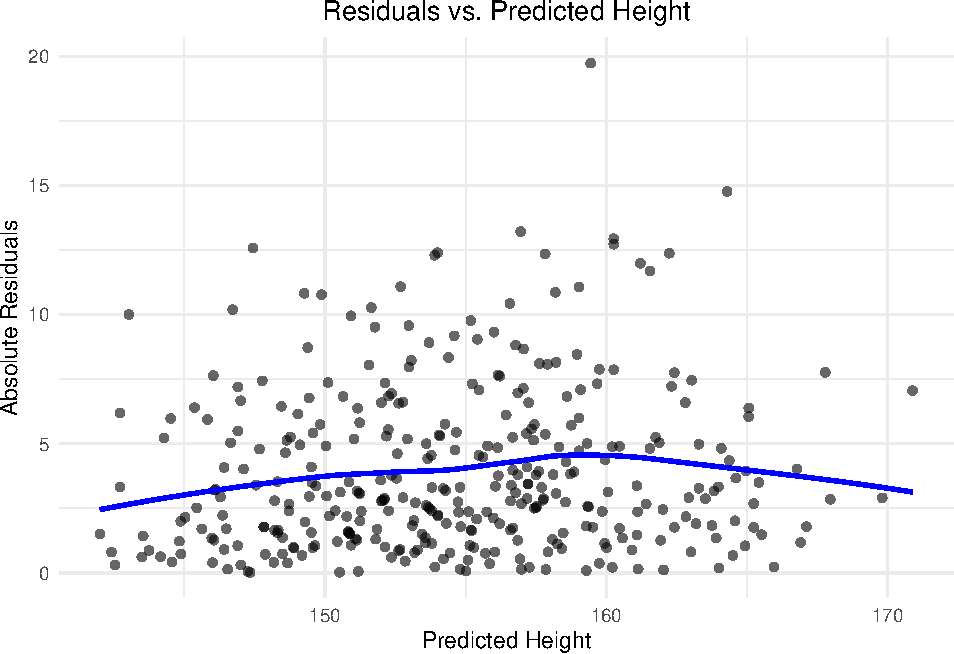
\includegraphics[keepaspectratio]{bookdown-demo_files/figure-latex/unnamed-chunk-47-1.pdf}}

\begin{verbatim}
## 479  94 
## 317  72
\end{verbatim}

With the 97\% confidence envelope, we can see if the residuals are
consistent with coming from a normal distribution.
We could again use simulation to see how the Q-Q Plot changes
to get a better feeling (see \hyperref[exercise9_simpl_lin_reg]{exercise 9}).

Another convenient way to check model assumptions (for a wide class of models)
is to use the \texttt{check\_model} function from the \texttt{performance} package:

\pandocbounded{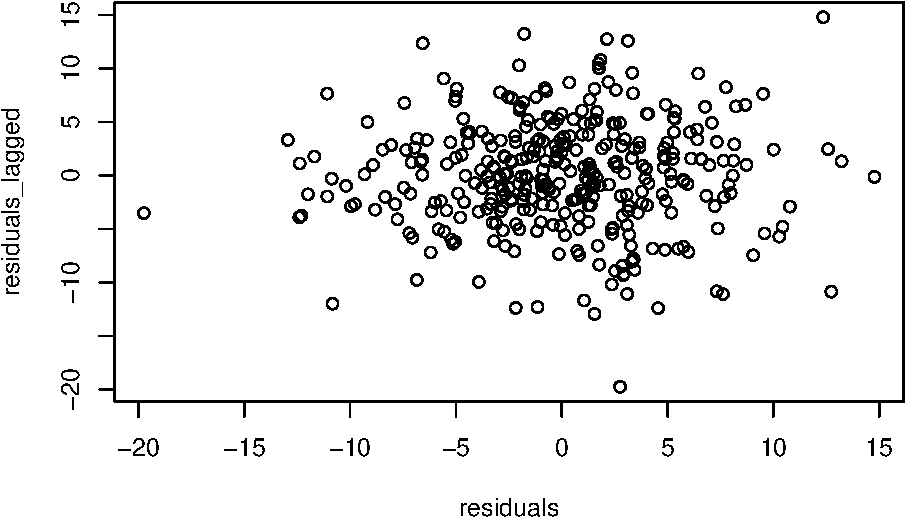
\includegraphics[keepaspectratio]{bookdown-demo_files/figure-latex/unnamed-chunk-48-1.pdf}}

In this case, everything looks fine. Let's go through the plots and explain them:

\paragraph{Posterior predictive check (upper left)}\label{posterior-predictive-check-upper-left}

Here, you create new data from the estimated model.
Using least squares, the estimated model was:
\[ height_i = 113.87939 + 0.90503 \cdot weight_i + Normal(0, 5.086) \]
From this model, we can simulate new data (or the original weights, if we want to use fixed X)
by plugging in different weights, and adding a random error from a normal distribution
with mean 0 and standard deviation 5.086.
Then, we can compare the distribution of the simulated data with the observed data.
The blue lines in the graph are model predicted heights, the green line are the
observed heights.

Let's try to replicate this plot.
First, we want to simulate new data from the model.
A scatter plot is also a nice way to check of the model predictions
are in line with the observed data. One could repeat this process
multiple times to get a feeling for the variability of the model predictions.

\begin{verbatim}
## `geom_smooth()` using formula = 'y ~ x'
\end{verbatim}

\pandocbounded{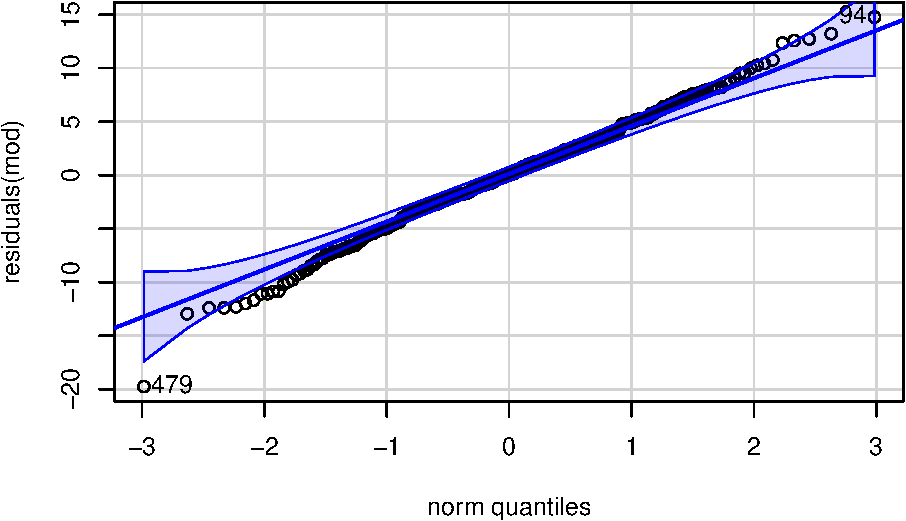
\includegraphics[keepaspectratio]{bookdown-demo_files/figure-latex/unnamed-chunk-49-1.pdf}}

The simulated and original data (green) fit nicely together.
This lends some credibility to the model.
And now the density plots of the model created data (blue) and the observed data (green):

\pandocbounded{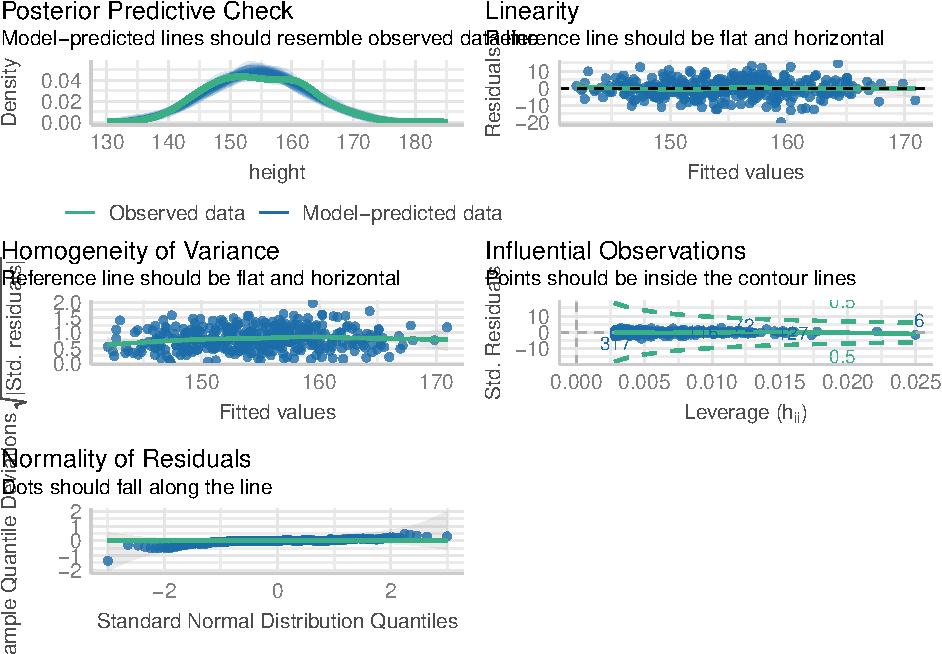
\includegraphics[keepaspectratio]{bookdown-demo_files/figure-latex/unnamed-chunk-50-1.pdf}}

As you can see, the densities of the observed and simulated data are broadly similar.
One could argue that heights in the range of 150-160 cm are a bit overestimated by the model.
Depending on the context, this might be a problem or not. Let's accept the model for now.

\paragraph{Linear fit (upper right)}\label{linear-fit-upper-right}

This is the same plot as \hyperref[linearity]{above}: \((\hat{y}_i, e_i)\).

\paragraph{Homogeneity of variance (middle left)}\label{homogeneity-of-variance-middle-left}

This is the same plot as \hyperref[constant_variance]{above}: \((\hat{y}_i, |e_i|)\).

\paragraph{Influential observations (middle right)}\label{influential-observations-middle-right}

The standard method to check for influential observations is to compute the
so-called \href{https://en.wikipedia.org/wiki/Cook\%27s_distance}{Cook's distance}.
This is a measure of how much leverage a single observation has on the model.
We can extract the Cook's distance from the model using \texttt{cooks.distance()}.
An ugly rule of thumb would be to look at observations with a Cook's distance
greater than 1.
In the plot, the leverage \(h_{ii}\) is on the x-axis, and the standardized residuals
are on the y-axis. In short, a high leverage means that the estimated value \(\hat{y}_i\)
is potentially far away from the original value \(y_i\).
The contours (dotted green lines) are the Cook's distance, in this
case at a Cook's distance of 0.5.
There is \href{https://en.wikipedia.org/wiki/Cook\%27s_distance\#Relationship_to_other_influence_measures_(and_interpretation)}{formula}
that relates the leverage (\(h_{ii}\)), the Cook's distance
and the residuals. Holding Cook`s distant constant at 0.5,
gives you the green dotted line in the plot.

Let's create an outlier and see what happens:

\pandocbounded{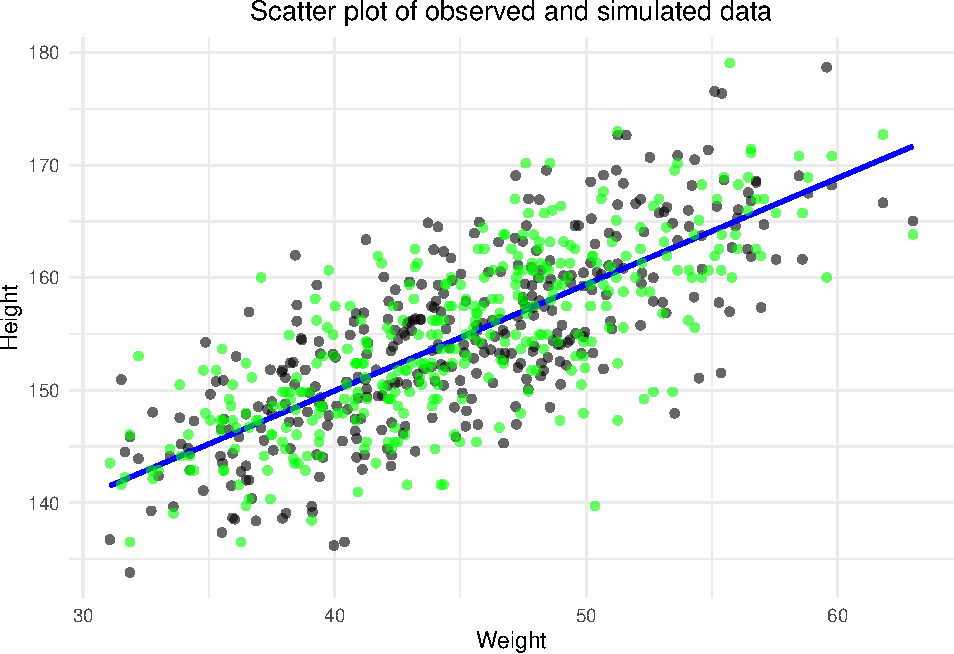
\includegraphics[keepaspectratio]{bookdown-demo_files/figure-latex/unnamed-chunk-51-1.pdf}}

\begin{verbatim}
## `geom_smooth()` using formula = 'y ~ x'
\end{verbatim}

\pandocbounded{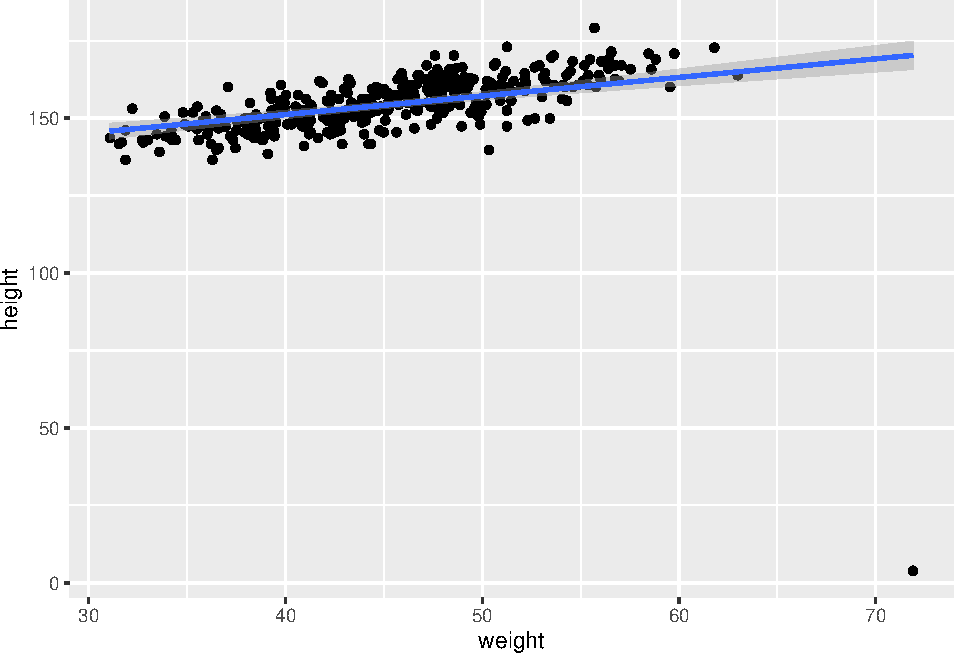
\includegraphics[keepaspectratio]{bookdown-demo_files/figure-latex/unnamed-chunk-51-2.pdf}}

\begin{verbatim}
## Cook's distance =  7.025207
\end{verbatim}

One single outlier changes the diagnostic plots. Observation 352
is clearly identified as influential. The one point
changes all diagnostic plots notably.
The estimates of the regression coefficients
are also affected:

\begin{verbatim}
## [1] "Original Model"
\end{verbatim}

\begin{verbatim}
## (Intercept)      weight 
## 113.8793936   0.9050291
\end{verbatim}

\begin{verbatim}
## [1] "Model with outlier"
\end{verbatim}

\begin{verbatim}
## (Intercept)      weight 
##  127.172494    0.599054
\end{verbatim}

Admitted, this is a somewhat artificial example.

\paragraph{Normality of residuals (lower left)}\label{normality-of-residuals-lower-left}

This is basically the same plot as above, just \href{https://cran.r-project.org/web/packages/qqplotr/vignettes/introduction.html}{detrended}.
Let's try to replicate it:

\begin{verbatim}
## 
## Attaching package: 'qqplotr'
\end{verbatim}

\begin{verbatim}
## The following objects are masked from 'package:ggplot2':
## 
##     stat_qq_line, StatQqLine
\end{verbatim}

\pandocbounded{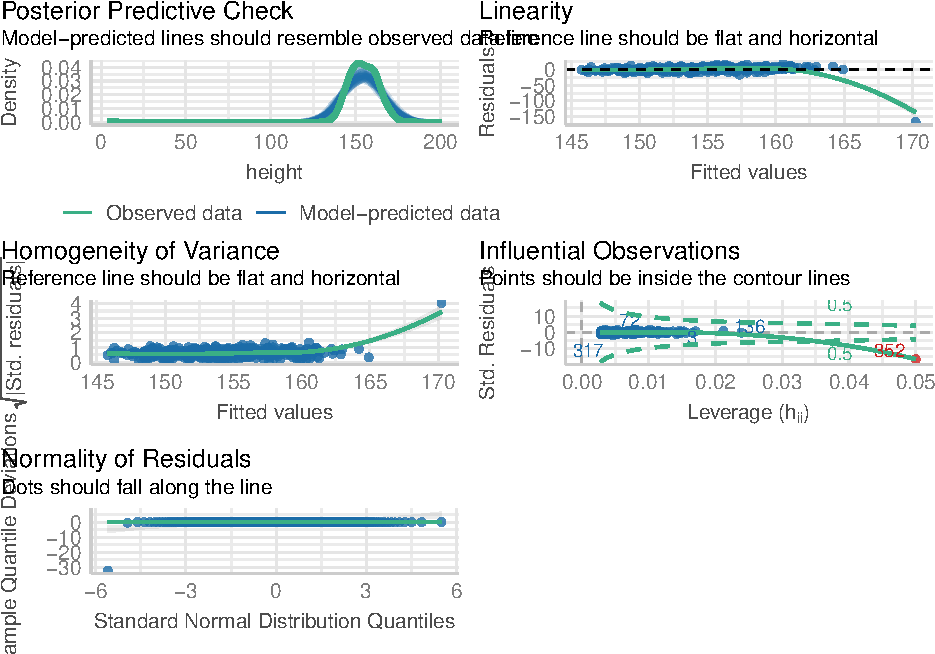
\includegraphics[keepaspectratio]{bookdown-demo_files/figure-latex/unnamed-chunk-53-1.pdf}}

The normality assumption seems to hold. Not that in the above QQ plot,
we detrended the residuals and used a bootrap confidence band. Depending
on the band type, the confidence band can be wider or narrower and include
or exclude points.

\textbf{After having checked the assumptions for the classical regression model}
and we feel comfortable with the model, we get exact confidence intervals
for the effect sizes (\(\beta\)s) using \texttt{confint()} (p.~74 in Westfall).

Heureka! We have a model that fits the data well.

\subsection{Bootstrap fit}\label{bootstrap-fit}

In order to get a feeling for the variability of the model with regards to the predictors as well,
we can bootstrap the whole data set, fit the model and draw regression lines.
We create \(100\) bootrap replicates of our data set \texttt{d2} by drawing with
replication. For every bootrap replicate, we fit the model and draw the regression line.

\pandocbounded{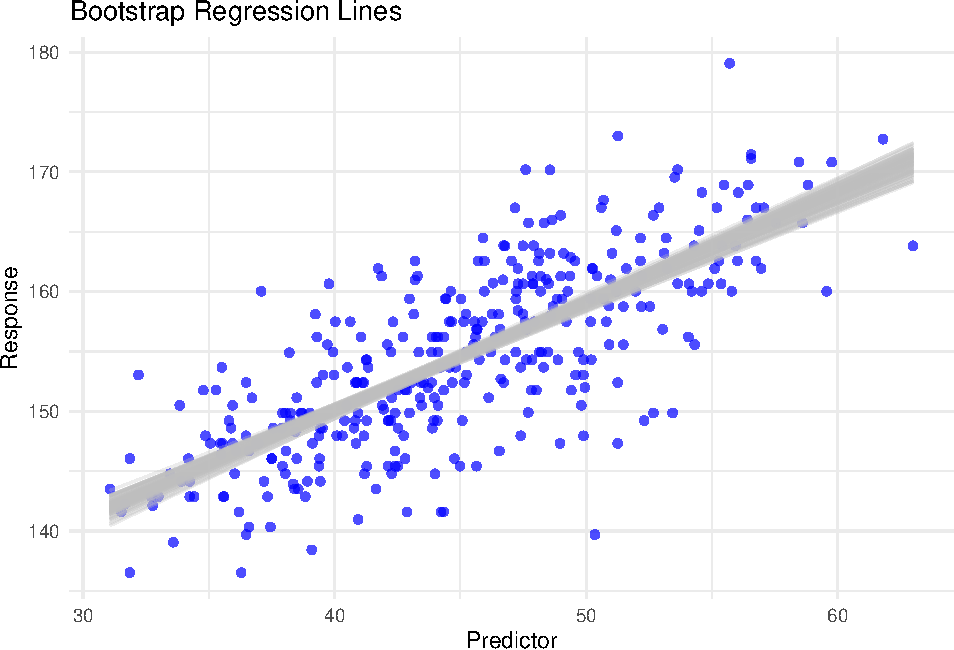
\includegraphics[keepaspectratio]{bookdown-demo_files/figure-latex/unnamed-chunk-54-1.pdf}}

The results is very stable. Neither intercept nor slope change much.

\subsection{Regression towards the mean}\label{regression-towards-the-mean}

There are great explanations for ``\href{https://en.wikipedia.org/wiki/Regression_toward_the_mean}{regression towards the mean}'' in
\href{http://www.stat.columbia.edu/~gelman/arm/}{Gelman} p.58 and
\href{https://www.routledge.com/Understanding-Regression-Analysis-A-Conditional-Distribution-Approach/Westfall-Arias/p/book/9780367493516?srsltid=AfmBOore3O_Ciecl0TTkr9AjPIY1d6OmbQa7o7IAdKpTSkD8s9HkwzD4}{Westfall} p.36.
This \href{https://www.youtube.com/watch?v=1tSqSMOyNFE&ab_channel=Veritasium}{video} might be interesting to watch.

It describes the phenomenon that the predicted value (y) is closer to its
mean than the predictor (x) its mean.
In our case this means, if the weight of a person is 1 standard deviation above the mean of body weights,
the (model-)predicted height is less than 1 standard deviation above the mean of body heights, but
still larger than the average height. Let's verify:

\begin{verbatim}
## predicted height= 0.7547479
\end{verbatim}

\begin{verbatim}
## `geom_smooth()` using formula = 'y ~ x'
\end{verbatim}

\pandocbounded{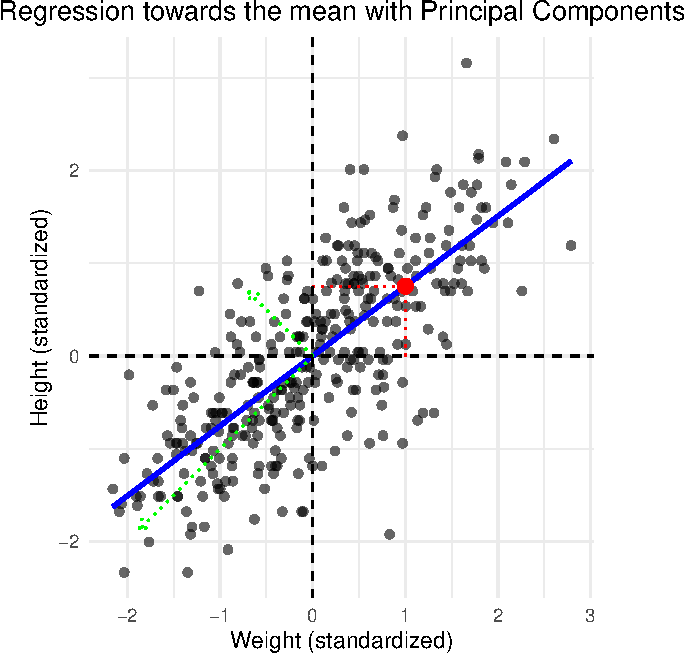
\includegraphics[keepaspectratio]{bookdown-demo_files/figure-latex/unnamed-chunk-55-1.pdf}}

As Gelman points out in his book (Figure 4.2), there is a fine detail:
The regression line is not the line most people would draw through the data.
They would draw a line through the main directions of variability
(directions are the eigenvectors of the covariance matrix).
In dotted green, you can see these directions. The regression line is a solution
to another problem (as we have seen): It minimizes the sum of squared residuals,
which are defined via the \textbf{vertical} distances to the line.
See \hyperref[exercise8_simpl_lin_reg]{exercise 8}.

\subsection{Random X vs fixed X}\label{random-x-vs-fixed-x}

A detail that is not mentioned often in introductory statistics courses
is the question of whether the predictor variable \(X\) is random or fixed.
In our case, we did not specify the weights of the people in the !Kung San data set.
\emph{Obervational} data was collected and we have no control over the weights.
In an \emph{experimental} setting, we could have controlled the weights of the people.
We could have for instance only included people with weights at certain steps (50 kg, 60 kg, 70 kg).
In the latter case, we could consider X as fixed. In the former case, we consider X as random.
Further reading: \href{https://www.routledge.com/Understanding-Regression-Analysis-A-Conditional-Distribution-Approach/Westfall-Arias/p/book/9780367493516?srsltid=AfmBOore3O_Ciecl0TTkr9AjPIY1d6OmbQa7o7IAdKpTSkD8s9HkwzD4}{Westfall} 1.5.

There are many more details we could look into, but we wanted to give a first
practical introduction to regression analysis with less empfahsis theory and proofs behind it.

\section{Exercises}\label{exercises-1}

\subsection{{[}E{]} Exercise 1}\label{exercise1_simpl_lin_reg}

In the model from above:

\begin{eqnarray*}
h_i &\sim& \text{Normal}(\mu_i, \sigma)\\
\mu_i &\sim& \alpha + \beta (x_i - \bar{x})\\
\alpha &\sim& \text{Normal}(171.1, 20)\\
\beta &\sim& \text{Normal}(0, 10)\\
\sigma &\sim& \text{Uniform}(0, 50)
\end{eqnarray*}

\begin{itemize}
\tightlist
\item
  What ist the expected height when \(x_i = \bar{x}\)?
\item
  What is the expected height when \(x_i\) changes by 1 unit?
\end{itemize}

\subsection{{[}E{]} Exercise 2}\label{exercise2_simpl_lin_reg}

Look at the marginal distrubutions of the parameters in the Bayesian model.

\begin{itemize}
\tightlist
\item
  Plot the posterior distribution of all 3 parameters.
\item
  Include in the plot a 99\% credible interval (HDI).
\end{itemize}

\subsection{{[}M{]} Exercise 3}\label{exercise3_simpl_lin_reg}

Go to the coefficient estimates in the simple linear regression setting
above (\hyperref[fit_model_simple_lin_reg_classic]{Fit the model})
in the classical framework.

\begin{itemize}
\tightlist
\item
  Create an R file to simulate the simple linear regression model.
\item
  Change your input parameters and see how the estimates change.
\item
  Does this make sense with respect to the estimates given, specifically with respect
  to \(\beta_1\)?
\end{itemize}

\subsection{{[}M{]} Exercise 4}\label{exercise4_simpl_lin_reg}

Verify the statement above in the text for high and low values of \(R^2\).

\subsection{{[}M{]} Exercise 5}\label{exercise5_simpl_lin_reg}

Verify with simulation in R that the separation of the distributions in the simple linear regression model
improves if the true (but usually unknown) slope increases.

\subsection{{[}H{]} Exercise 6}\label{exercise6_simpl_lin_reg}

Go to the model assumptions in the classical regression model (\hyperref[_model_assumptions]{Model Assumptions}).
- Use the code from \href{https://github.com/jdegenfellner/Script_QM2_ZHAW/blob/main/02-Simple_Linear_Regression.Rmd}{github}
to recreate the regression model with the sine-curve.
- Check the independence assumption as described. Look at the residuals, when \(X=2\) and \(X=4.5\).
You can get those by filtering residuals that are \(>0.5\) and \(<0.5\).

\subsection{{[}M{]} Exercise 7}\label{exercise7_simpl_lin_reg}

\begin{itemize}
\tightlist
\item
  Simulate data from the regression of heights on weights in our !Kung San data set.
\item
  Draw the \(\hat{y_i}, e_i\) plot.
\item
  Draw the \(\hat{y_i}, |e_i|\) plot.
\item
  Repeat the simulation and look at the variability of the plot.
\end{itemize}

\subsection{{[}H{]} Exercise 8}\label{exercise8_simpl_lin_reg}

\begin{itemize}
\tightlist
\item
  Go to p.36 in Westfall's book and read Appendix A.
\item
  Pay close attention to the explanation about regression toward the mean.
\end{itemize}

\subsection{{[}M{]} Exercise 9}\label{exercise9_simpl_lin_reg}

Go to the resuials \hyperref[normality_assumption]{above} where we tested the normality assumption.

\begin{itemize}
\tightlist
\item
  Calcuate mean and standard deviation from the residuals of the model
  that regresses height on weight.
\item
  Simulate from a normal distribution using these parameters.
\item
  Get a feeling how the QQ plot changes by drawing the QQ plot repeatedly.
\end{itemize}

\subsection{{[}M{]} Exercise 10}\label{exercise10_simpl_lin_reg}

Using our !Kung San data,

\begin{itemize}
\tightlist
\item
  show that the regression of height on weight (\texttt{lm(height\ \textasciitilde{}\ weight)})
  is not the same as the regression of weight on height (\texttt{lm(weight\ \textasciitilde{}\ height)}).
\item
  Draw both regression lines in one diagram.
\item
  Can you simulate data where the two regressions deliver (almost) identical results?
\item
  Explain why the results differ and what consequences this would have for a research question.
  Which question do I answer with each?
\end{itemize}

\subsection{{[}E{]} Exercise 11}\label{exercise11_simpl_lin_reg}

Go back to the \hyperref[seperating_property]{section} about \(R^2\) and the separation of the distributions.
How would the probability that a person in the 90\% quantile of the weight
is taller than a person in the 10\% quantile of the weight change if you change

\begin{itemize}
\tightlist
\item
  the true slope of the regression line
\item
  the true \(\sigma\), i.e.~if you add more noise and have a lower \(R^2\)?
\end{itemize}

\chapter{Multiple Linear Regression}\label{multiple-linear-regression}

So far, we have dealt with the simple mean model and the model with one predictor
in the Bayesian and Frequentist framework.
We will now add another predictor and subsequently an interaction term to the model.

\section{Linear Regression with 2 Predictors in the Baysian Framework}\label{linear-regression-with-2-predictors-in-the-baysian-framework}

\subsection{Meaning of ``linear''}\label{meaning-of-linear}

What is a linear model? The term ``linear'' refers to the relationship of the predictors
with the dependent variable (or outcome). The following model is also linear:

\[height_i = \beta_0 + \beta_1 x_i + \beta_2 x_i^2\]

The model is linear in the parameters \(\beta_0, \beta_1, \beta_2\) but not in the predictors \(x_i\).
The term \(x_i^2\) is ok, since the heights are just sums of multiples of the predictors (which can be nonlinear).
This model is not a linear model anymore:

\[height_i = \beta_0 + \beta_1 x_i + e^{\beta_2 x_i^2}\]

\(\beta_2\) is now is the exponent of \(e\). It would also not be linear,
if the coefficients are in a square root or in the denominator of a fraction,
or in a sine or in a logarithm. You get the idea.

\subsection{Adding a transformed predictor to the model}\label{adding_transformed_predictor}

The world is not flat, although some people on YouTube might tell you otherwise.
In our context, not all regression is linear.

Around 4.5. in the book \href{https://civil.colorado.edu/~balajir/CVEN6833/bayes-resources/RM-StatRethink-Bayes.pdf}{Statistical Rethinking}
there is are lineare regression using a quadratic term for weight.
It is a principle, called the ``\textbf{variable inclusion principle}'', that we always include the lower order terms when fitting a model
with higher order terms. See \href{https://vdoc.pub/documents/understanding-regression-analysis-a-conditional-distribution-approach-84oqjr8sqva0}{Westfall},
p.~213. If we do not include the lower order terms, the coefficient does not measure what
we want it to meausure (curvature in our case). For instance, if we want to model a quadratic relationship (parabola) between
weight and height, we also have to include the linear term for weight (\(x_i\)).
Since we do not assume the relationship between weight and height to be linear but
quadratic (which is a polynomial of degree 2), we call this a
\href{https://en.wikipedia.org/wiki/Polynomial_regression\#:~:text=In\%20statistics\%2C\%20polynomial\%20regression\%20is,nth\%20degree\%20polynomial\%20in\%20x.}{polynomial regression}.

This time, lets look at the whole age range of data from the !Kung San people.

\begin{Shaded}
\begin{Highlighting}[]
\FunctionTok{library}\NormalTok{(rethinking)}
\FunctionTok{library}\NormalTok{(tidyverse)}
\FunctionTok{data}\NormalTok{(Howell1)}
\NormalTok{d }\OtherTok{\textless{}{-}}\NormalTok{ Howell1}
\NormalTok{d }\SpecialCharTok{\%\textgreater{}\%} \FunctionTok{ggplot}\NormalTok{(}\FunctionTok{aes}\NormalTok{(}\AttributeTok{x =}\NormalTok{ weight, }\AttributeTok{y =}\NormalTok{ height)) }\SpecialCharTok{+}
  \FunctionTok{geom\_point}\NormalTok{() }\SpecialCharTok{+}
  \FunctionTok{geom\_smooth}\NormalTok{(}\AttributeTok{method =} \StringTok{"lm"}\NormalTok{, }\AttributeTok{se =} \ConstantTok{FALSE}\NormalTok{, }\AttributeTok{color =} \StringTok{"blue"}\NormalTok{) }\SpecialCharTok{+}
  \FunctionTok{geom\_smooth}\NormalTok{(}\AttributeTok{method =} \StringTok{"loess"}\NormalTok{, }\AttributeTok{se =} \ConstantTok{FALSE}\NormalTok{, }\AttributeTok{color =} \StringTok{"red"}\NormalTok{)}
\end{Highlighting}
\end{Shaded}

\begin{verbatim}
## `geom_smooth()` using formula = 'y ~ x'
## `geom_smooth()` using formula = 'y ~ x'
\end{verbatim}

\pandocbounded{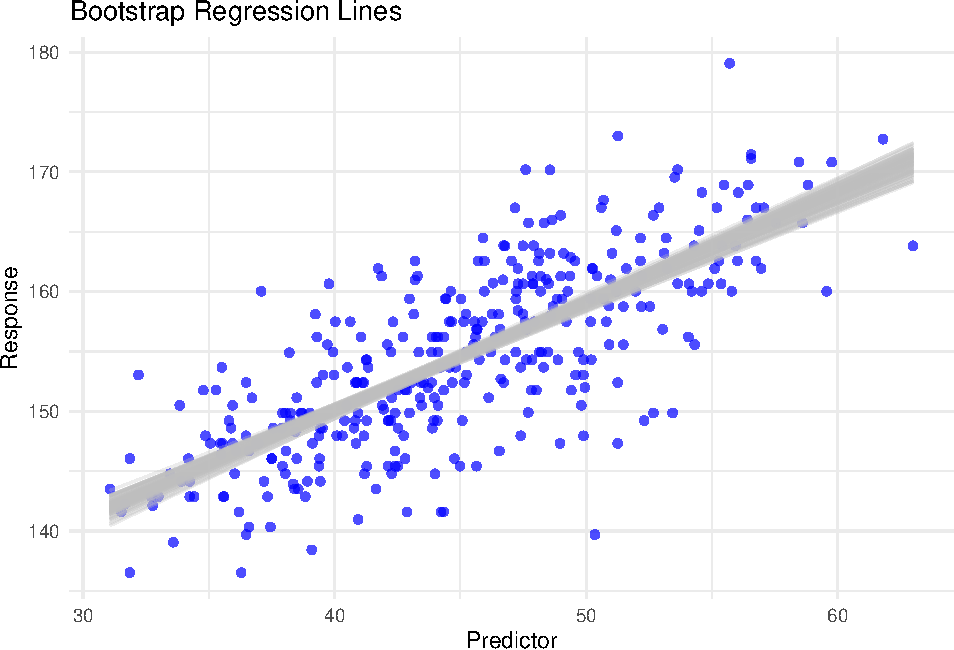
\includegraphics[keepaspectratio]{bookdown-demo_files/figure-latex/unnamed-chunk-56-1.pdf}}

It would not be a good idea to fit a linear trend through this data,
because we would not caupture the relationship adequately.
The red line is a \href{https://en.wikipedia.org/wiki/Local_regression}{loess smothing} line
which is often used to capture non-linear relationships.
The blue line is the usual line from classic linear regression (from the previous chapter).
Which one describes the data more accurately?
In this case it is obvious, a non-linear relationship is present and it might be a good idea
to model it. Modeling the relationshiop with a linear trend, leads to bad residuals with structure.
We will demonstrate this in the freuqentist setting.
Unfortunately, in more complex settings, with more predictors, it is not always so easy to see.

This time, we use the mean for the prior from the book (\(178 cm\)).
The model equations are (see \hyperref[exercise2_multiple_regression]{exercise 2}):

\begin{eqnarray*}
h_i &\sim& \text{Normal}(\mu_i, \sigma) \\
\mu_i &=& \alpha + \beta_1 x_i + \beta_2 x_i^2 \\
\alpha &\sim& \text{Normal}(178, 20) \\
\beta_1 &\sim& \text{Log-Normal}(0, 1) \\
\beta_2 &\sim& \text{Normal}(0, 1) \\
\sigma &\sim& \text{Uniform}(0, 50)
\end{eqnarray*}

The prior for \(\beta_1\) is log-normal, because we can reasonably assume
the the overall linear trend is positive. The prior for \(\beta_2\) is normal, because
we are not so sure. If we thought back to our school days to the topic of
``curve discussion'' or parabolas, we could probably also assume that \(\beta_2\) is negative.
But, data will show.

How can we interpret the model equations?
The model assumes that the \textbf{expected} height \(\mu_i\) of a person \(i\)
depends non-linearly on the weight \(x_i\) of the person.
We are in the business of mean-modeling.
The prior for \(\sigma\) is uniform as before.
The prior for \(\alpha\) is normal with mean \(178\) and standard deviation \(20\)
because this is what we can expect from body heights in our experience.

Let's \textbf{fit the model}:

We standardize the weight again and add the squared weights to the data set.
Standardizing the the predictors is a good idea, especially in polynomial regression
since squares and cubes of large numbers can get huge and cause numerical problems.

Let's fit the model with the quadratic term for weight:

\begin{Shaded}
\begin{Highlighting}[]
\CommentTok{\# Standardize weight}
\NormalTok{d}\SpecialCharTok{$}\NormalTok{weight\_s }\OtherTok{\textless{}{-}}\NormalTok{ (d}\SpecialCharTok{$}\NormalTok{weight }\SpecialCharTok{{-}} \FunctionTok{mean}\NormalTok{(d}\SpecialCharTok{$}\NormalTok{weight)) }\SpecialCharTok{/} \FunctionTok{sd}\NormalTok{(d}\SpecialCharTok{$}\NormalTok{weight)}
\CommentTok{\# Square of standardized weight}
\NormalTok{d}\SpecialCharTok{$}\NormalTok{weight\_s2 }\OtherTok{\textless{}{-}}\NormalTok{ d}\SpecialCharTok{$}\NormalTok{weight\_s}\SpecialCharTok{\^{}}\DecValTok{2}
\NormalTok{m4}\FloatTok{.1} \OtherTok{\textless{}{-}} \FunctionTok{quap}\NormalTok{(}
  \FunctionTok{alist}\NormalTok{(}
\NormalTok{    height }\SpecialCharTok{\textasciitilde{}} \FunctionTok{dnorm}\NormalTok{(mu, sigma),}
\NormalTok{    mu }\OtherTok{\textless{}{-}}\NormalTok{ a }\SpecialCharTok{+}\NormalTok{ b1}\SpecialCharTok{*}\NormalTok{weight\_s }\SpecialCharTok{+}\NormalTok{ b2}\SpecialCharTok{*}\NormalTok{weight\_s}\SpecialCharTok{\^{}}\DecValTok{2}\NormalTok{,}
\NormalTok{    a }\SpecialCharTok{\textasciitilde{}} \FunctionTok{dnorm}\NormalTok{(}\DecValTok{178}\NormalTok{, }\DecValTok{20}\NormalTok{),}
\NormalTok{    b1 }\SpecialCharTok{\textasciitilde{}} \FunctionTok{dnorm}\NormalTok{(}\DecValTok{0}\NormalTok{, }\DecValTok{10}\NormalTok{),}
\NormalTok{    b2 }\SpecialCharTok{\textasciitilde{}} \FunctionTok{dnorm}\NormalTok{(}\DecValTok{0}\NormalTok{, }\DecValTok{10}\NormalTok{),}
\NormalTok{    sigma }\SpecialCharTok{\textasciitilde{}} \FunctionTok{dunif}\NormalTok{(}\DecValTok{0}\NormalTok{, }\DecValTok{50}\NormalTok{)}
\NormalTok{  ), }\AttributeTok{data =}\NormalTok{ d)}
\FunctionTok{precis}\NormalTok{(m4}\FloatTok{.1}\NormalTok{)}
\end{Highlighting}
\end{Shaded}

\begin{verbatim}
##             mean        sd       5.5%      94.5%
## a     146.672739 0.3736465 146.075580 147.269898
## b1     21.397637 0.2898827  20.934348  21.860925
## b2     -8.419933 0.2813308  -8.869554  -7.970312
## sigma   5.750550 0.1743749   5.471865   6.029235
\end{verbatim}

\(\beta_2\) is indeed negative.
We get our \textbf{\href{https://en.wikipedia.org/wiki/Joint_probability_distribution}{joint distribution}}
of the \textbf{four model parameters}.
Let's look at the fit using the mean estimates of the posterior distribution:

\begin{Shaded}
\begin{Highlighting}[]
\CommentTok{\# Summarize the model parameters}
\NormalTok{model\_summary }\OtherTok{\textless{}{-}} \FunctionTok{precis}\NormalTok{(m4}\FloatTok{.1}\NormalTok{)}
\NormalTok{params }\OtherTok{\textless{}{-}} \FunctionTok{as.data.frame}\NormalTok{(model\_summary)}

\CommentTok{\# Extract parameter values}
\NormalTok{a }\OtherTok{\textless{}{-}}\NormalTok{ params[}\StringTok{"a"}\NormalTok{, }\StringTok{"mean"}\NormalTok{]       }\CommentTok{\# Intercept}
\NormalTok{b1 }\OtherTok{\textless{}{-}}\NormalTok{ params[}\StringTok{"b1"}\NormalTok{, }\StringTok{"mean"}\NormalTok{]     }\CommentTok{\# Coefficient for standardized weight}
\NormalTok{b2 }\OtherTok{\textless{}{-}}\NormalTok{ params[}\StringTok{"b2"}\NormalTok{, }\StringTok{"mean"}\NormalTok{]     }\CommentTok{\# Coefficient for squared standardized weight}

\CommentTok{\# Generate a sequence of standardized weights for the fitted curve}
\NormalTok{weight\_fine }\OtherTok{\textless{}{-}} \FunctionTok{seq}\NormalTok{(}\FunctionTok{min}\NormalTok{(d}\SpecialCharTok{$}\NormalTok{weight\_s), }\FunctionTok{max}\NormalTok{(d}\SpecialCharTok{$}\NormalTok{weight\_s), }\AttributeTok{length.out =} \DecValTok{200}\NormalTok{)}

\CommentTok{\# Calculate the fitted values using the quadratic equation}
\NormalTok{height\_fitted }\OtherTok{\textless{}{-}}\NormalTok{ a }\SpecialCharTok{+}\NormalTok{ b1 }\SpecialCharTok{*}\NormalTok{ weight\_fine }\SpecialCharTok{+}\NormalTok{ b2 }\SpecialCharTok{*}\NormalTok{ weight\_fine}\SpecialCharTok{\^{}}\DecValTok{2}

\CommentTok{\# Plot the scatterplot}
\FunctionTok{plot}\NormalTok{(d}\SpecialCharTok{$}\NormalTok{weight\_s, d}\SpecialCharTok{$}\NormalTok{height, }\AttributeTok{pch =} \DecValTok{16}\NormalTok{, }\AttributeTok{col =} \StringTok{"blue"}\NormalTok{,}
     \AttributeTok{xlab =} \StringTok{"Standardized Weight"}\NormalTok{, }\AttributeTok{ylab =} \StringTok{"Height (cm)"}\NormalTok{,}
     \AttributeTok{main =} \StringTok{"Scatterplot with Fitted Curve (Standardized Weight)"}\NormalTok{)}

\CommentTok{\# Add the fitted curve}
\FunctionTok{lines}\NormalTok{(weight\_fine, height\_fitted, }\AttributeTok{col =} \StringTok{"red"}\NormalTok{, }\AttributeTok{lwd =} \DecValTok{2}\NormalTok{)}

\CommentTok{\# Add a legend}
\FunctionTok{legend}\NormalTok{(}\StringTok{"topright"}\NormalTok{, }\AttributeTok{legend =} \FunctionTok{c}\NormalTok{(}\StringTok{"Observed data"}\NormalTok{, }\StringTok{"Fitted curve"}\NormalTok{),}
       \AttributeTok{col =} \FunctionTok{c}\NormalTok{(}\StringTok{"blue"}\NormalTok{, }\StringTok{"red"}\NormalTok{), }\AttributeTok{pch =} \FunctionTok{c}\NormalTok{(}\DecValTok{16}\NormalTok{, }\ConstantTok{NA}\NormalTok{), }\AttributeTok{lty =} \FunctionTok{c}\NormalTok{(}\ConstantTok{NA}\NormalTok{, }\DecValTok{1}\NormalTok{), }\AttributeTok{lwd =} \DecValTok{2}\NormalTok{)}
\end{Highlighting}
\end{Shaded}

\pandocbounded{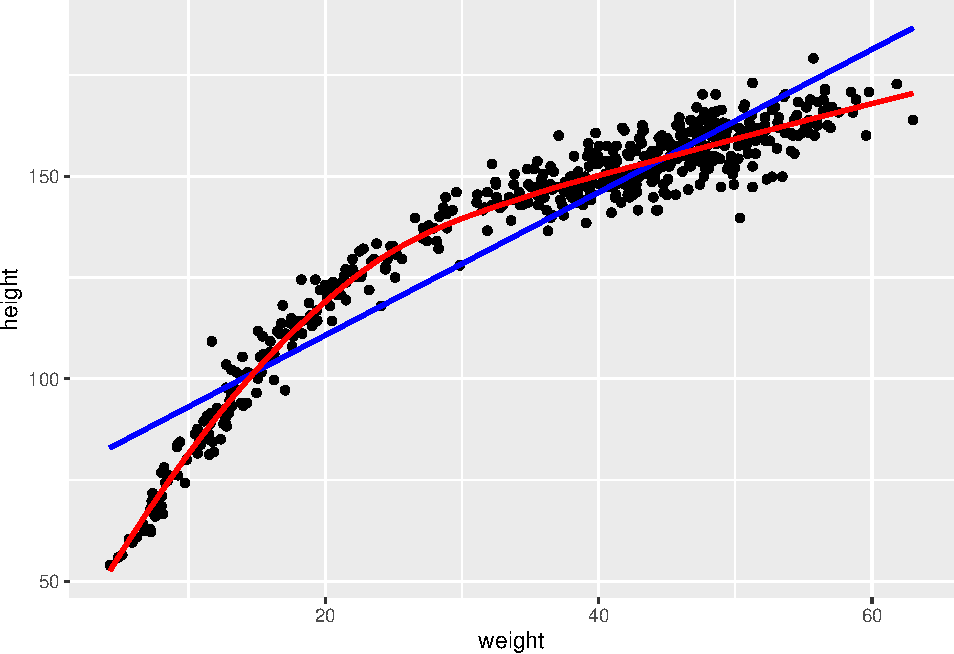
\includegraphics[keepaspectratio]{bookdown-demo_files/figure-latex/unnamed-chunk-58-1.pdf}}

This fits much better than the linear model. In the book,
there is also a polynomial regression with a cubic term for weight.
Maybe this fits even better (see \hyperref[exercise1_multiple_regression]{exercise 1}).

\subsection{Adding another predictor to the model}\label{adding_predictor_bayes}

Since the !Kung San data set has already such a high \(R^2\) with the quadratic term
(and possibly higher with the cubic term), we will use the created data set from
\hyperref[adding_predictor_freq]{below} in the frequentist setting
to estimate the coefficients of the model with two predictors.

We use rather uniformative priors and fit the model using \texttt{quap}:

\begin{Shaded}
\begin{Highlighting}[]
\FunctionTok{library}\NormalTok{(rethinking)}
\FunctionTok{set.seed}\NormalTok{(}\DecValTok{123}\NormalTok{)}
\NormalTok{n }\OtherTok{\textless{}{-}} \DecValTok{100}
\NormalTok{X1 }\OtherTok{\textless{}{-}} \FunctionTok{rnorm}\NormalTok{(n, }\DecValTok{0}\NormalTok{, }\DecValTok{5}\NormalTok{)}
\NormalTok{X2 }\OtherTok{\textless{}{-}} \FunctionTok{rnorm}\NormalTok{(n, }\DecValTok{0}\NormalTok{, }\DecValTok{5}\NormalTok{)}
\NormalTok{Y }\OtherTok{\textless{}{-}} \DecValTok{10} \SpecialCharTok{+} \FloatTok{0.5} \SpecialCharTok{*}\NormalTok{ X1 }\SpecialCharTok{+} \DecValTok{1} \SpecialCharTok{*}\NormalTok{ X2 }\SpecialCharTok{+} \FunctionTok{rnorm}\NormalTok{(n, }\DecValTok{0}\NormalTok{, }\DecValTok{2}\NormalTok{) }\CommentTok{\# true model}
\NormalTok{df }\OtherTok{\textless{}{-}} \FunctionTok{data.frame}\NormalTok{(}\AttributeTok{X1 =}\NormalTok{ X1, }\AttributeTok{X2 =}\NormalTok{ X2, }\AttributeTok{Y =}\NormalTok{ Y)}

\CommentTok{\# fit model}
\NormalTok{m4}\FloatTok{.2} \OtherTok{\textless{}{-}} \FunctionTok{quap}\NormalTok{(}
  \FunctionTok{alist}\NormalTok{(}
\NormalTok{    Y }\SpecialCharTok{\textasciitilde{}} \FunctionTok{dnorm}\NormalTok{(mu, sigma),}
\NormalTok{    mu }\OtherTok{\textless{}{-}}\NormalTok{ a }\SpecialCharTok{+}\NormalTok{ b1}\SpecialCharTok{*}\NormalTok{X1 }\SpecialCharTok{+}\NormalTok{ b2}\SpecialCharTok{*}\NormalTok{X2,}
\NormalTok{    a }\SpecialCharTok{\textasciitilde{}} \FunctionTok{dnorm}\NormalTok{(}\DecValTok{10}\NormalTok{, }\DecValTok{10}\NormalTok{),}
\NormalTok{    b1 }\SpecialCharTok{\textasciitilde{}} \FunctionTok{dnorm}\NormalTok{(}\DecValTok{0}\NormalTok{, }\DecValTok{10}\NormalTok{),}
\NormalTok{    b2 }\SpecialCharTok{\textasciitilde{}} \FunctionTok{dnorm}\NormalTok{(}\DecValTok{0}\NormalTok{, }\DecValTok{10}\NormalTok{),}
\NormalTok{    sigma }\SpecialCharTok{\textasciitilde{}} \FunctionTok{dunif}\NormalTok{(}\DecValTok{0}\NormalTok{, }\DecValTok{50}\NormalTok{)}
\NormalTok{  ), }\AttributeTok{data =}\NormalTok{ df)}
\FunctionTok{precis}\NormalTok{(m4}\FloatTok{.2}\NormalTok{)}
\end{Highlighting}
\end{Shaded}

\begin{verbatim}
##             mean         sd      5.5%      94.5%
## a     10.2700227 0.18934442 9.9674137 10.5726316
## b1     0.4467278 0.04131434 0.3806995  0.5127561
## b2     1.0095082 0.03899992 0.9471788  1.0718377
## sigma  1.8738833 0.13250803 1.6621099  2.0856567
\end{verbatim}

\subsubsection{Checking model assumptions}\label{check_model_bayes}

Andrew Gelman mentions in some of his talks (see \href{https://sites.stat.columbia.edu/gelman/research/published/philosophy_chapter.pdf}{here} for more details)
that many Bayesians he met do not check their models, since they reflect subjective probability.
As I said in the introduction, one should not be afraid to check model predictions against the observed
and probably new data. If a model for predicting BMI performs much worse on a new data set,
we can probably conclude that the model does not reflect the general relationship between the predictors
and the dependent variable. We \textbf{do not ask} the question if a model is true or false, but if it is useful or
how badly the model assumptions are violated.

For further, more detailed information on model checking, refer to chapter 6 of
\href{https://sites.stat.columbia.edu/gelman/book/BDA3.pdf}{Gelman's book}.

Anyhow, we plot two posterior predictive checks here.
We test the model within the same data set. We create new observations
by drawing from the posterior distribution and compare these with the acutally
observed values. This is called \textbf{posterior predictive checks}.

\textbf{First, we plot the observed \(Y\) values against the predicted \(Y\) values (\(=\hat{Y}\))}
from the model (as in Statistical rethinking, Chapter 5).
Although these practically never lie on the line \(y=x\), they should be sufficiently
close to it. We could also compare these two plots with the mean-model (see \hyperref[exercise6_multiple_regression]{exercise 6}).

\begin{Shaded}
\begin{Highlighting}[]
\CommentTok{\# 1) Posterior predictive checks Y vs Y\_hat}
\CommentTok{\# see Statstical Rethinking p 138.}
\CommentTok{\# call link without specifying new data}
\CommentTok{\# so it uses the original data}
\NormalTok{mu }\OtherTok{\textless{}{-}} \FunctionTok{link}\NormalTok{(m4}\FloatTok{.2}\NormalTok{)}

\CommentTok{\# summarize samples accross cases}
\NormalTok{mu\_mean }\OtherTok{\textless{}{-}} \FunctionTok{apply}\NormalTok{(mu, }\DecValTok{2}\NormalTok{, mean)}
\NormalTok{mu\_PI }\OtherTok{\textless{}{-}} \FunctionTok{apply}\NormalTok{(mu, }\DecValTok{2}\NormalTok{, PI, }\AttributeTok{prob =} \FloatTok{0.89}\NormalTok{)}

\CommentTok{\# simulate observations}
\CommentTok{\# again, no new data, so uses original data}
\NormalTok{D\_sim }\OtherTok{\textless{}{-}} \FunctionTok{sim}\NormalTok{(m4}\FloatTok{.2}\NormalTok{, }\AttributeTok{n =} \FloatTok{1e4}\NormalTok{)}
\NormalTok{D\_PI }\OtherTok{\textless{}{-}} \FunctionTok{apply}\NormalTok{(D\_sim, }\DecValTok{2}\NormalTok{, PI, }\AttributeTok{prob =} \FloatTok{0.89}\NormalTok{)}

\FunctionTok{plot}\NormalTok{(mu\_mean }\SpecialCharTok{\textasciitilde{}}\NormalTok{ df}\SpecialCharTok{$}\NormalTok{Y, }\AttributeTok{col =}\NormalTok{ rangi2, }\AttributeTok{ylim =} \FunctionTok{range}\NormalTok{(mu\_PI), }
     \AttributeTok{xlab =} \StringTok{"Observed Y"}\NormalTok{, }\AttributeTok{ylab =} \StringTok{"Model{-}Predicted Y"}\NormalTok{)}
\FunctionTok{abline}\NormalTok{(}\AttributeTok{a =} \DecValTok{0}\NormalTok{, }\AttributeTok{b =} \DecValTok{1}\NormalTok{, }\AttributeTok{lty =} \DecValTok{2}\NormalTok{)}
\ControlFlowTok{for}\NormalTok{(i }\ControlFlowTok{in} \DecValTok{1}\SpecialCharTok{:}\FunctionTok{nrow}\NormalTok{(df)) }\FunctionTok{lines}\NormalTok{(}\FunctionTok{rep}\NormalTok{(df}\SpecialCharTok{$}\NormalTok{Y[i], }\DecValTok{2}\NormalTok{), mu\_PI[,i], }\AttributeTok{col =}\NormalTok{ rangi2)}
\end{Highlighting}
\end{Shaded}

\pandocbounded{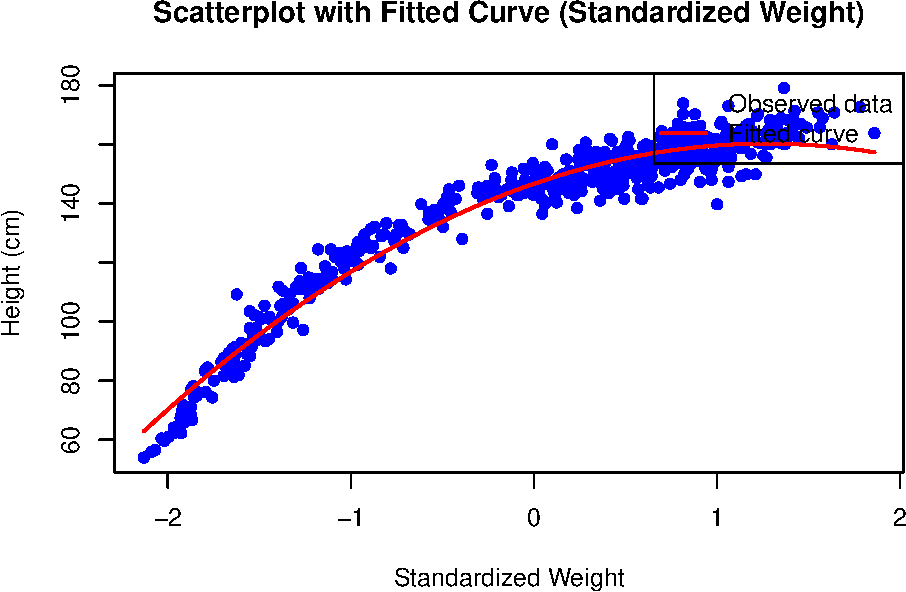
\includegraphics[keepaspectratio]{bookdown-demo_files/figure-latex/unnamed-chunk-60-1.pdf}}

As we can see, the model fits the data quite well. The points are close to the dashed line (\(y=x\)).
No under- or overestimation is visible. The model seems to capture the relationship between the predictors \(X_1\) and \(X_2\)
and the dependent variable \(Y\) quite well. If there were patches of data points above or below the dashed line,
we would probably have to reconsider the model definition and think about why these points are not captured by the model.

\textbf{Next, we plot the posterior predictive plots} analog to the upper left in the \texttt{check\_model} output.

\begin{Shaded}
\begin{Highlighting}[]
\FunctionTok{library}\NormalTok{(scales)  }\CommentTok{\# For the alpha function to adjust transparency}
\end{Highlighting}
\end{Shaded}

\begin{verbatim}
## 
## Attaching package: 'scales'
\end{verbatim}

\begin{verbatim}
## The following object is masked from 'package:purrr':
## 
##     discard
\end{verbatim}

\begin{verbatim}
## The following object is masked from 'package:readr':
## 
##     col_factor
\end{verbatim}

\begin{Shaded}
\begin{Highlighting}[]
\CommentTok{\# 2) Posterior predictive densities}
\CommentTok{\# Simulate observations using the posterior predictive distribution}
\NormalTok{D\_sim }\OtherTok{\textless{}{-}} \FunctionTok{sim}\NormalTok{(m4}\FloatTok{.2}\NormalTok{, }\AttributeTok{n =} \FloatTok{1e4}\NormalTok{)  }\CommentTok{\# Generate 10,000 simulated datasets}

\CommentTok{\# Calculate densities for all samples}
\NormalTok{densities }\OtherTok{\textless{}{-}} \FunctionTok{apply}\NormalTok{(D\_sim, }\DecValTok{1}\NormalTok{, density)}

\CommentTok{\# Find the maximum density value for setting the y{-}axis limits}
\NormalTok{max\_density }\OtherTok{\textless{}{-}} \FunctionTok{max}\NormalTok{(}\FunctionTok{sapply}\NormalTok{(densities, }\ControlFlowTok{function}\NormalTok{(d) }\FunctionTok{max}\NormalTok{(d}\SpecialCharTok{$}\NormalTok{y)))}

\CommentTok{\# Create the density plot with predefined ylim}
\FunctionTok{plot}\NormalTok{(}\ConstantTok{NULL}\NormalTok{, }\AttributeTok{xlim =} \FunctionTok{range}\NormalTok{(df}\SpecialCharTok{$}\NormalTok{Y), }\AttributeTok{ylim =} \FunctionTok{c}\NormalTok{(}\DecValTok{0}\NormalTok{, max\_density),}
     \AttributeTok{xlab =} \StringTok{"Y"}\NormalTok{, }\AttributeTok{ylab =} \StringTok{"Density"}\NormalTok{,}
     \AttributeTok{main =} \StringTok{"Comparison of Observed and Predicted Densities"}\NormalTok{)}

\CommentTok{\# Add 100 posterior predictive density lines}
\FunctionTok{set.seed}\NormalTok{(}\DecValTok{42}\NormalTok{)  }\CommentTok{\# For reproducibility}
\NormalTok{n\_lines }\OtherTok{\textless{}{-}} \DecValTok{100}
\NormalTok{samples }\OtherTok{\textless{}{-}} \FunctionTok{sample}\NormalTok{(}\DecValTok{1}\SpecialCharTok{:}\FloatTok{1e4}\NormalTok{, n\_lines)  }\CommentTok{\# Randomly sample 100 posterior predictive datasets}
\ControlFlowTok{for}\NormalTok{ (s }\ControlFlowTok{in}\NormalTok{ samples) \{}
  \FunctionTok{lines}\NormalTok{(}\FunctionTok{density}\NormalTok{(D\_sim[s, ]), }\AttributeTok{col =} \FunctionTok{alpha}\NormalTok{(}\StringTok{"lightblue"}\NormalTok{, }\FloatTok{0.3}\NormalTok{), }\AttributeTok{lwd =} \DecValTok{1}\NormalTok{)}
\NormalTok{\}}

\CommentTok{\# Add the density line for the observed Y values}
\NormalTok{obs\_density }\OtherTok{\textless{}{-}} \FunctionTok{density}\NormalTok{(df}\SpecialCharTok{$}\NormalTok{Y)}
\FunctionTok{lines}\NormalTok{(obs\_density}\SpecialCharTok{$}\NormalTok{x, obs\_density}\SpecialCharTok{$}\NormalTok{y, }\AttributeTok{col =} \StringTok{"green"}\NormalTok{, }\AttributeTok{lwd =} \DecValTok{2}\NormalTok{)}

\CommentTok{\# Add legend}
\FunctionTok{legend}\NormalTok{(}\StringTok{"topright"}\NormalTok{, }\AttributeTok{legend =} \FunctionTok{c}\NormalTok{(}\StringTok{"Posterior Predictive Densities"}\NormalTok{, }\StringTok{"Observed Density"}\NormalTok{),}
       \AttributeTok{col =} \FunctionTok{c}\NormalTok{(}\StringTok{"lightblue"}\NormalTok{, }\StringTok{"green"}\NormalTok{), }\AttributeTok{lty =} \DecValTok{1}\NormalTok{, }\AttributeTok{lwd =} \FunctionTok{c}\NormalTok{(}\DecValTok{1}\NormalTok{, }\DecValTok{2}\NormalTok{))}
\end{Highlighting}
\end{Shaded}

\pandocbounded{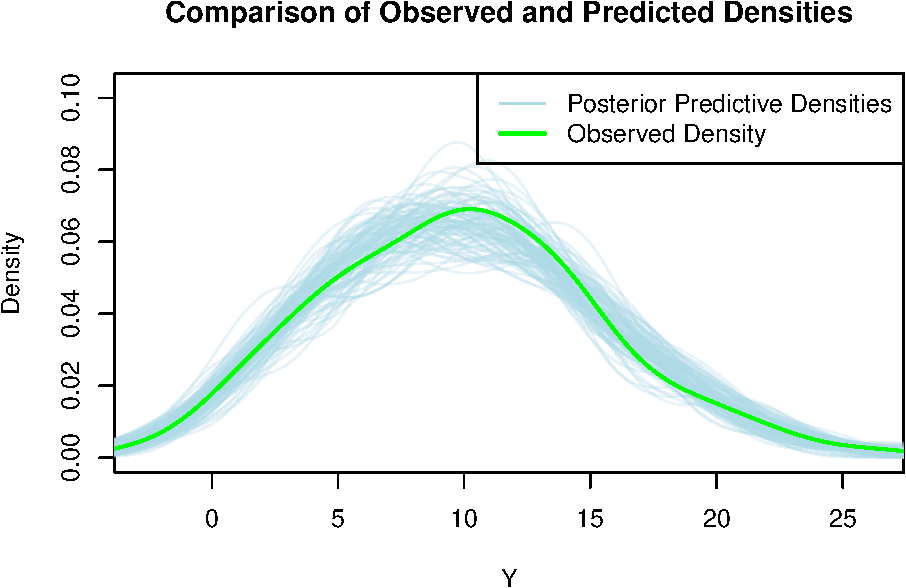
\includegraphics[keepaspectratio]{bookdown-demo_files/figure-latex/unnamed-chunk-61-1.pdf}}

The light blue lines show distributions of model predicted \(Y\) values.
The green line shows the distribution of the observed \(Y\) values.
As we can see, there seem to be no systematic differences between the observed and predicted values.
The model seems to capture the relationship well.
If we see systematic deviations here, we need to reconsider the model definition.

\textbf{Example}: If you want to predict pain (\(Y\) variable) and you have a lot of zeros (pain-free participants)
you will probably see a discrepancy between the observed and predicted values in this plot.
What could you do? You could use a two step process (model the probability that a person is pain-free
and then model the pain intensity for the people who have pain) or use a different model (like a zero-inflated model).

Note that we did not explicitely assume normally distributed errors in the model definition above,
so we won't check this here but in the Frequentist framework below.

\section{Linear regression with 2 Predictors in the Frequentist Framework}\label{linear-regression-with-2-predictors-in-the-frequentist-framework}

\subsection{Adding a transformed predictor to the model}\label{adding-a-transformed-predictor-to-the-model}

No, let's fit the same model as above in the frequentist framework.

The model is:

\[height_i = \alpha + \beta_1 weight_i + \beta_2 weight_i^2 + \varepsilon_i\]
whereas
\[\varepsilon_i \sim N(0, \sigma)\]

We are looking for fixed, but unknown, parameters \(\alpha\), \(\beta_1\), \(\beta_2\) and \(\sigma\).
This is fit again using the \texttt{lm} function in R which uses least squares to estimate the parameters.
At this point I could torture you with \href{https://en.wikipedia.org/wiki/Matrix_(mathematics)}{matrix algebra}
and show you the \href{https://en.wikipedia.org/wiki/Linear_least_squares}{normal equations} for linear regression,
but I will spare you for now.
Note that the least squares algorithm for fitting the curve works for all
kinds of functions. We could also fit an exponential curve using the same
technique.

\begin{Shaded}
\begin{Highlighting}[]
\CommentTok{\# scale weight}
\NormalTok{d}\SpecialCharTok{$}\NormalTok{weight\_s }\OtherTok{\textless{}{-}} \FunctionTok{scale}\NormalTok{(d}\SpecialCharTok{$}\NormalTok{weight)}
\CommentTok{\# Fit the model}
\NormalTok{m4}\FloatTok{.2} \OtherTok{\textless{}{-}} \FunctionTok{lm}\NormalTok{(height }\SpecialCharTok{\textasciitilde{}}\NormalTok{ weight\_s }\SpecialCharTok{+} \FunctionTok{I}\NormalTok{(weight\_s}\SpecialCharTok{\^{}}\DecValTok{2}\NormalTok{), }\AttributeTok{data =}\NormalTok{ d)}
\FunctionTok{summary}\NormalTok{(m4}\FloatTok{.2}\NormalTok{)}
\end{Highlighting}
\end{Shaded}

\begin{verbatim}
## 
## Call:
## lm(formula = height ~ weight_s + I(weight_s^2), data = d)
## 
## Residuals:
##      Min       1Q   Median       3Q      Max 
## -19.9689  -3.9794   0.2364   3.9262  19.5182 
## 
## Coefficients:
##               Estimate Std. Error t value Pr(>|t|)    
## (Intercept)   146.6604     0.3748  391.30   <2e-16 ***
## weight_s       21.4149     0.2908   73.64   <2e-16 ***
## I(weight_s^2)  -8.4123     0.2822  -29.80   <2e-16 ***
## ---
## Signif. codes:  0 '***' 0.001 '**' 0.01 '*' 0.05 '.' 0.1 ' ' 1
## 
## Residual standard error: 5.766 on 541 degrees of freedom
## Multiple R-squared:  0.9565, Adjusted R-squared:  0.9564 
## F-statistic:  5952 on 2 and 541 DF,  p-value: < 2.2e-16
\end{verbatim}

See \texttt{?I} in R. This command is used so that R knows that it should
treat the ``\^{}2'' as ``square'' and not as formula syntax.
We could also create a new variable as before. Whatever you prefer.

\subsubsection{Interpretation of output and coefficients}\label{interpretation-of-output-and-coefficients}

\begin{itemize}
\tightlist
\item
  The intercept \(\alpha\) is the \textbf{model-predicted height} of a person of \textbf{average weight}.
  Note that this is not the average height of the people in the data set, since the
  mean model is also a model, but different from ours.
\item
  The residuals have range from \(-19.97\) to \(19.51\). So, the model maximally
  overestimates the heights by \(19.97\) cm and underestimates by \(19.51\) cm.
  These numbers are plausible when you look at the scatterplot with the fitted
  curve.
\item
  The coefficients \(\beta_1\) and \(\beta_2\) agree with the Bayes estimates.
  Specifically, \(\beta_2\) is non-zero indicating curvature.
\item
  If you like \(p\)-values: All the hypotheses that the coefficients are zero
  are rejected. The \(p\)-values are very small. The data can not be explained
  by chance alone. On the other hand, for at least \(\beta_1\) and
  and the global test this is not a surprise when you look at the scatterplot.
\item
  The \(R^2\) is a whopping \(0.96\) which could be a sign of overfitting, but
  in this case we conclude that the true relationship is caputured rather well.
  \href{https://en.wikipedia.org/wiki/Overfitting}{Overfitting} would occur if
  our curve would wiggle around the data points,
  so we would fit the data too much to the noise in the data than
  the underying trend.
\end{itemize}

\subsubsection{Checking model assumptions}\label{checking-model-assumptions}

\begin{Shaded}
\begin{Highlighting}[]
\FunctionTok{check\_model}\NormalTok{(m4}\FloatTok{.2}\NormalTok{)}
\end{Highlighting}
\end{Shaded}

\begin{verbatim}
## Some of the variables were in matrix-format - probably you used
##   `scale()` on your data?
##   If so, and you get an error, please try `datawizard::standardize()` to
##   standardize your data.
## Some of the variables were in matrix-format - probably you used
##   `scale()` on your data?
##   If so, and you get an error, please try `datawizard::standardize()` to
##   standardize your data.
\end{verbatim}

\pandocbounded{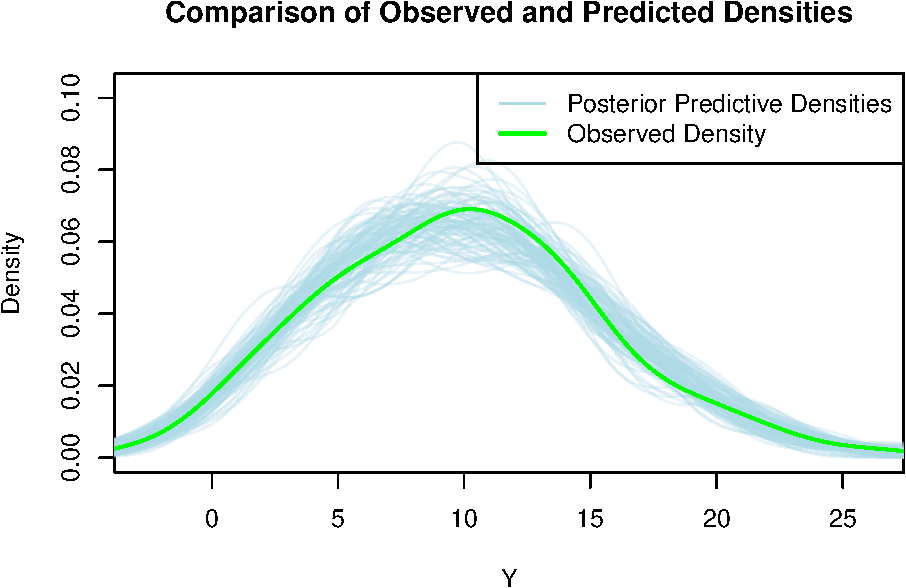
\includegraphics[keepaspectratio]{bookdown-demo_files/figure-latex/unnamed-chunk-63-1.pdf}}

If we want to be perfectionists, we could remark that (upper right plot)
in the lower fitted values the residuals are more negative,
meaning that the model overestimates the heights in this region.
In the middle region the model underestimates a bit and we can see
a positive tendency in the residuals. Apart from that,
the diagnostic plots look excellent.

\subsection{Adding another predictor to the model}\label{adding_predictor_freq}

Now, we add another predictor to the model. We use \(X_1\) and \(X_2\)
\textbf{simultaneously} to predict \(Y\). We are now in the lucky situation that
we can still visualize the situation in 3D. The regression line from simple
linear regression
becomes a \href{https://stackoverflow.com/questions/47344850/scatterplot3d-regression-plane-with-residuals}{plane}.
The vertical distances between the data points and the plane are the residuals.
See \href{https://rpubs.com/pjozefek/576206}{here} or
\href{https://www.sthda.com/english/wiki/scatterplot3d-3d-graphics-r-software-and-data-visualization}{here}
at the end for examples.
Minimizing the sum of the squared errors gives again
the estimates for the coefficients.

For demonstration purposes, we can \textbf{create data ourselves} with known
coefficients. This is the same as \hyperref[adding_predictor_bayes]{above}.
This is the true model, which we usually do not know:

\[ Y_i = \beta_0 + \beta_1 X_{1i} + \beta_2 X_{2i} + \varepsilon_i\]
\[ \varepsilon_i \sim N(0, \sigma^2)\]
\[ \mathbb{E}(Y_i|X_1 = x_1; X_2 = x_2) = \beta_0 + \beta_1 x_1 + \beta_2 x_2\]
\[ i = 1 \ldots n\]

for example:

\[ Y_i = 10 + 0.5 \cdot X_{1i} + 1 \cdot X_{2i} + \varepsilon_i\]
\[ \varepsilon_i \sim N(0, 5)\]
\[ \mathbb{E}(Y_i|X_1 = x_1; X_2 = x_2) = 10 + 0.5 x_1 + 1 x_2\]
\[ i = 1 \ldots n\]

According to the model, the conditional expected value of \(Y_i\) given \(X_1 = x_1\) and \(X_2 = x_2\)
is a linear function of \(x_1\) and \(x_2\). Note, that small letters are realized values
of random variables. Also note, that in the expectation the error term goes away, since
\(\mathbb{E}(\varepsilon_i) = 0\).

\begin{itemize}
\tightlist
\item
  If \(X_1\) increases by one unit, \(Y\) increases by \(0.5\) units on average (in expectation).
\item
  If \(X_2\) increases by one unit, \(Y\) increases by \(1\) unit on average (in expectation).
\item
  If \(X_1\) and \(X_2\) are zero, \(Y\) is \(10\) on average (in expectation).
\end{itemize}

Why in expectation? Because there is still the error term which makes the whole thing random!
We can see that an increase in \(X_1\) does not influence the relationship between \(X_2\) and \(Y\).
Hence, there is \textbf{no interaction} between \(X_1\) and \(X_2\) with respect to \(Y\).

Now lets's draw 100 points from this model, fit the model and add the plane:

\begin{Shaded}
\begin{Highlighting}[]
\FunctionTok{library}\NormalTok{(plotly)}

\FunctionTok{set.seed}\NormalTok{(}\DecValTok{123}\NormalTok{)}
\NormalTok{n }\OtherTok{\textless{}{-}} \DecValTok{100}
\NormalTok{X1 }\OtherTok{\textless{}{-}} \FunctionTok{rnorm}\NormalTok{(n, }\DecValTok{0}\NormalTok{, }\DecValTok{5}\NormalTok{)}
\NormalTok{X2 }\OtherTok{\textless{}{-}} \FunctionTok{rnorm}\NormalTok{(n, }\DecValTok{0}\NormalTok{, }\DecValTok{5}\NormalTok{)}
\NormalTok{Y }\OtherTok{\textless{}{-}} \DecValTok{10} \SpecialCharTok{+} \FloatTok{0.5} \SpecialCharTok{*}\NormalTok{ X1 }\SpecialCharTok{+} \DecValTok{1} \SpecialCharTok{*}\NormalTok{ X2 }\SpecialCharTok{+} \FunctionTok{rnorm}\NormalTok{(n, }\DecValTok{0}\NormalTok{, }\DecValTok{2}\NormalTok{)}
\NormalTok{d }\OtherTok{\textless{}{-}} \FunctionTok{data.frame}\NormalTok{(}\AttributeTok{X1 =}\NormalTok{ X1, }\AttributeTok{X2 =}\NormalTok{ X2, }\AttributeTok{Y =}\NormalTok{ Y)}

\CommentTok{\# Fit the model}
\NormalTok{m4}\FloatTok{.3} \OtherTok{\textless{}{-}} \FunctionTok{lm}\NormalTok{(Y }\SpecialCharTok{\textasciitilde{}}\NormalTok{ X1 }\SpecialCharTok{+}\NormalTok{ X2, }\AttributeTok{data =}\NormalTok{ d)}
\FunctionTok{summary}\NormalTok{(m4}\FloatTok{.3}\NormalTok{)}
\end{Highlighting}
\end{Shaded}

\begin{verbatim}
## 
## Call:
## lm(formula = Y ~ X1 + X2, data = d)
## 
## Residuals:
##     Min      1Q  Median      3Q     Max 
## -3.7460 -1.3215 -0.2489  1.2427  4.1597 
## 
## Coefficients:
##             Estimate Std. Error t value Pr(>|t|)    
## (Intercept) 10.27013    0.19228   53.41   <2e-16 ***
## X1           0.44673    0.04195   10.65   <2e-16 ***
## X2           1.00952    0.03960   25.49   <2e-16 ***
## ---
## Signif. codes:  0 '***' 0.001 '**' 0.01 '*' 0.05 '.' 0.1 ' ' 1
## 
## Residual standard error: 1.903 on 97 degrees of freedom
## Multiple R-squared:  0.8839, Adjusted R-squared:  0.8815 
## F-statistic: 369.1 on 2 and 97 DF,  p-value: < 2.2e-16
\end{verbatim}

\begin{Shaded}
\begin{Highlighting}[]
\CommentTok{\# Create a grid for the plane}
\NormalTok{X1\_grid }\OtherTok{\textless{}{-}} \FunctionTok{seq}\NormalTok{(}\FunctionTok{min}\NormalTok{(d}\SpecialCharTok{$}\NormalTok{X1), }\FunctionTok{max}\NormalTok{(d}\SpecialCharTok{$}\NormalTok{X1), }\AttributeTok{length.out =} \DecValTok{20}\NormalTok{)}
\NormalTok{X2\_grid }\OtherTok{\textless{}{-}} \FunctionTok{seq}\NormalTok{(}\FunctionTok{min}\NormalTok{(d}\SpecialCharTok{$}\NormalTok{X2), }\FunctionTok{max}\NormalTok{(d}\SpecialCharTok{$}\NormalTok{X2), }\AttributeTok{length.out =} \DecValTok{20}\NormalTok{)}
\NormalTok{grid }\OtherTok{\textless{}{-}} \FunctionTok{expand.grid}\NormalTok{(}\AttributeTok{X1 =}\NormalTok{ X1\_grid, }\AttributeTok{X2 =}\NormalTok{ X2\_grid)}

\CommentTok{\# Predict the values for the grid}
\NormalTok{grid}\SpecialCharTok{$}\NormalTok{Y }\OtherTok{\textless{}{-}} \FunctionTok{predict}\NormalTok{(m4}\FloatTok{.3}\NormalTok{, }\AttributeTok{newdata =}\NormalTok{ grid)}

\CommentTok{\# Convert the grid into a matrix for the plane}
\NormalTok{plane\_matrix }\OtherTok{\textless{}{-}} \FunctionTok{matrix}\NormalTok{(grid}\SpecialCharTok{$}\NormalTok{Y, }\AttributeTok{nrow =} \FunctionTok{length}\NormalTok{(X1\_grid), }\AttributeTok{ncol =} \FunctionTok{length}\NormalTok{(X2\_grid))}

\CommentTok{\# Create the interactive 3D plot}
\FunctionTok{plot\_ly}\NormalTok{() }\SpecialCharTok{\%\textgreater{}\%}
  \FunctionTok{add\_markers}\NormalTok{(}
    \AttributeTok{x =}\NormalTok{ d}\SpecialCharTok{$}\NormalTok{X2, }\AttributeTok{y =}\NormalTok{ d}\SpecialCharTok{$}\NormalTok{X1, }\AttributeTok{z =}\NormalTok{ d}\SpecialCharTok{$}\NormalTok{Y,}
    \AttributeTok{marker =} \FunctionTok{list}\NormalTok{(}\AttributeTok{color =} \StringTok{"blue"}\NormalTok{, }\AttributeTok{size =} \DecValTok{5}\NormalTok{),}
    \AttributeTok{name =} \StringTok{"Data Points"}
\NormalTok{  ) }\SpecialCharTok{\%\textgreater{}\%}
  \FunctionTok{add\_surface}\NormalTok{(}
    \AttributeTok{x =}\NormalTok{ X1\_grid, }\AttributeTok{y =}\NormalTok{ X2\_grid, }\AttributeTok{z =}\NormalTok{ plane\_matrix,}
    \AttributeTok{colorscale =} \FunctionTok{list}\NormalTok{(}\FunctionTok{c}\NormalTok{(}\DecValTok{0}\NormalTok{, }\DecValTok{1}\NormalTok{), }\FunctionTok{c}\NormalTok{(}\StringTok{"red"}\NormalTok{, }\StringTok{"pink"}\NormalTok{)),}
    \AttributeTok{showscale =} \ConstantTok{FALSE}\NormalTok{,}
    \AttributeTok{opacity =} \FloatTok{0.7}\NormalTok{,}
    \AttributeTok{name =} \StringTok{"Fitted Plane"}
\NormalTok{  ) }\SpecialCharTok{\%\textgreater{}\%}
\NormalTok{  plotly}\SpecialCharTok{::}\FunctionTok{layout}\NormalTok{(}
    \AttributeTok{scene =} \FunctionTok{list}\NormalTok{(}
      \AttributeTok{xaxis =} \FunctionTok{list}\NormalTok{(}\AttributeTok{title =} \StringTok{"X1"}\NormalTok{),}
      \AttributeTok{yaxis =} \FunctionTok{list}\NormalTok{(}\AttributeTok{title =} \StringTok{"X2"}\NormalTok{),}
      \AttributeTok{zaxis =} \FunctionTok{list}\NormalTok{(}\AttributeTok{title =} \StringTok{"Y"}\NormalTok{)}
\NormalTok{    ),}
    \AttributeTok{title =} \StringTok{"Interactive 3D Scatterplot with Fitted Plane"}
\NormalTok{  )}
\end{Highlighting}
\end{Shaded}

\begin{verbatim}
## file:////private/var/folders/pm/jd6n6gj10371_bml1gh8sc5w0000gn/T/RtmpkK6ULT/file57f6f75410c/widget57f65b0182c1.html screenshot completed
\end{verbatim}

\pandocbounded{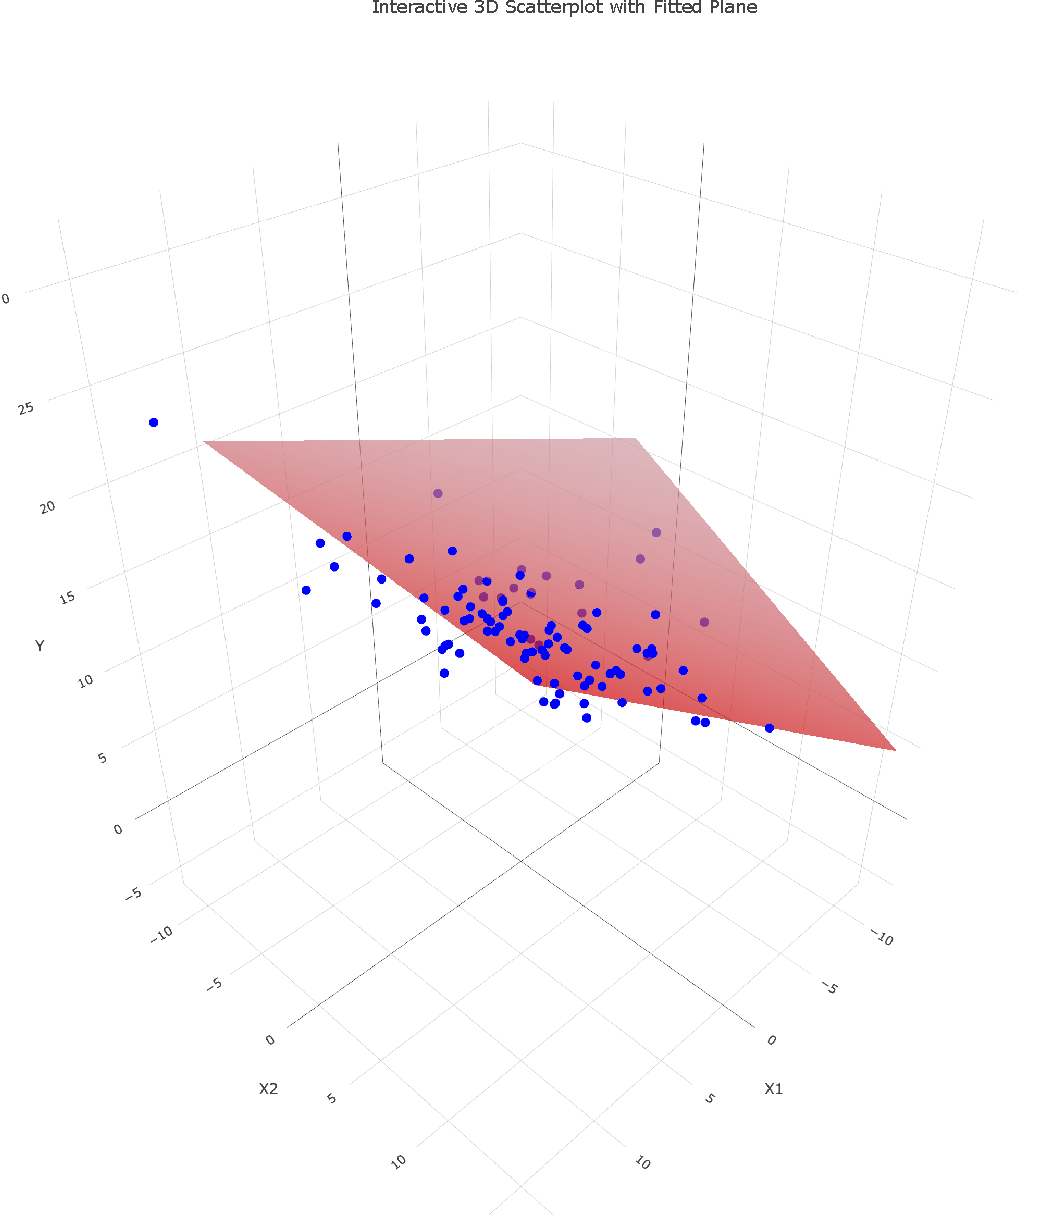
\includegraphics[keepaspectratio]{bookdown-demo_files/figure-latex/unnamed-chunk-64-1.pdf}}

This is, of course, a very idealized situation. There is no curvature in the plane,
no interaction, no outliers, no heteroscadasticity. It's the simplest case of multiple regression
with 2 predictors. Reality is - usually - more complicated.

Let's look at summary output and check model assumptions:

\begin{Shaded}
\begin{Highlighting}[]
\FunctionTok{summary}\NormalTok{(m4}\FloatTok{.3}\NormalTok{)}
\end{Highlighting}
\end{Shaded}

\begin{verbatim}
## 
## Call:
## lm(formula = Y ~ X1 + X2, data = d)
## 
## Residuals:
##     Min      1Q  Median      3Q     Max 
## -3.7460 -1.3215 -0.2489  1.2427  4.1597 
## 
## Coefficients:
##             Estimate Std. Error t value Pr(>|t|)    
## (Intercept) 10.27013    0.19228   53.41   <2e-16 ***
## X1           0.44673    0.04195   10.65   <2e-16 ***
## X2           1.00952    0.03960   25.49   <2e-16 ***
## ---
## Signif. codes:  0 '***' 0.001 '**' 0.01 '*' 0.05 '.' 0.1 ' ' 1
## 
## Residual standard error: 1.903 on 97 degrees of freedom
## Multiple R-squared:  0.8839, Adjusted R-squared:  0.8815 
## F-statistic: 369.1 on 2 and 97 DF,  p-value: < 2.2e-16
\end{verbatim}

\begin{Shaded}
\begin{Highlighting}[]
\FunctionTok{check\_model}\NormalTok{(m4}\FloatTok{.3}\NormalTok{)}
\end{Highlighting}
\end{Shaded}

\pandocbounded{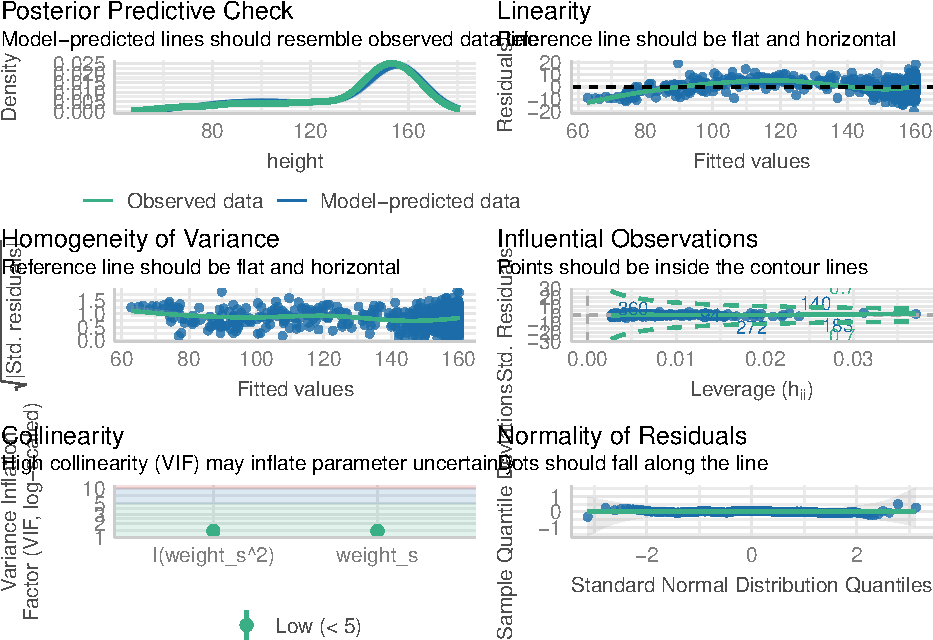
\includegraphics[keepaspectratio]{bookdown-demo_files/figure-latex/unnamed-chunk-65-1.pdf}}

We could repeat this simulation to get a feeling for the variability.
The posterior predictive checks look nice. In this case, we \emph{know} that the model is true
and with this knowledge we can assess the diagnostic plots in front of us.

\subsubsection{Adding variables to the model and why}\label{adding-variables-to-the-model-and-why}

This is a very complex question. We will go into it in later chapters and the next course (Methodenvertiefung).
At this point we can say this:
Depending on the goal at hand (prediction or explanation), we add variables to the model and probably use
other models apart from linear regression.
Prediction seems to be easier than explanation. For instance, within linear models and
just a handful of predictors, one can even brute force the problem by searching through
all subsets of predictors. If that is not possible, one could use clever algortithms, like
\href{https://www.sthda.com/english/articles/37-model-selection-essentials-in-r/155-best-subsets-regression-essentials-in-r/}{best subest selection}.

\begin{itemize}
\tightlist
\item
  What is \textbf{not} a good idea is to throw all variables into the model and hope for the best.
\item
  What is also not a good idea is to select variables depending on the \(p\)-values of the coefficients.
\item
  \textbf{Leaving variables out}, that are important, can lead to biased estimates of the coefficients
  (\href{https://en.wikipedia.org/wiki/Omitted-variable_bias}{omitted variable bias}).
\item
  But also \textbf{adding variables} can hurt conclusions from the model (see Statistical Rethinking 6.2).
\end{itemize}

\subsection{\texorpdfstring{Interaction Term \(X_1 \times X_2\)}{Interaction Term X\_1 \textbackslash times X\_2}}\label{interaction_term}

I recommend reading the excellent explanations about interactions
in John Kruschke's book \href{https://nyu-cdsc.github.io/learningr/assets/kruschke_bayesian_in_R.pdf}{Doing Bayesian Data Analysis},
15.2.2 und 15.2.3. Peter Westfall also has a nice explanation in his \href{https://www.routledge.com/Understanding-Regression-Analysis-A-Conditional-Distribution-Approach/Westfall-Arias/p/book/9780367493516?srsltid=AfmBOore3O_Ciecl0TTkr9AjPIY1d6OmbQa7o7IAdKpTSkD8s9HkwzD4}{book}
in section 9.3.

Our statistical model is now:

\[ Y_i = \beta_0 + \beta_1 X_{1i} + \beta_2 X_{2i} + \mathbf{\beta_3 X_{1i} \times X_{2i}} + \varepsilon_i\]
\[ \varepsilon_i \sim N(0, \sigma^2)\]
\[ \mathbb{E}(Y_i|X_1 = x_1; X_2 = x_2) = \beta_0 + \beta_1 x_{1} + \beta_2 x_{2} + \beta_3 x_{1} \times x_{2}\]
\[ i = 1 \ldots n\]

for example:

\[ Y_i = 10 + 0.5 \cdot X_{1i} + 1 \cdot X_{2i} + 0.89 \cdot X_{1i} \times X_{2i} + \varepsilon_i\]
\[ \varepsilon_i \sim N(0, 5)\]
\[ \mathbb{E}(Y_i|X_1 = x_1; X_2 = x_2) = 10 + 0.5 x_1 + 1 x_2 + 0.89 x_1 \times x_2\]
\[ i = 1 \ldots n\]

The second equation states that the conditional expectation of \(Y_i\) given \(X_1=x_1\) and \(X_2=x_2\)
is a function of \(x_1\) and \(x_2\) and their interaction \(x_1 \times x_2\). We are in a different situation now.
Set for instance \(x_2\) to a certain value, say \(x_2 = 7\). Then the relationship (in expectation)
between \(Y\) and \(X_1\) is:

\[ \mathbb{E}(Y_i|X_1 = x_1; X_2 = 7) = 10 + 0.5 x_1 + 1 \cdot 7 + 0.89 x_1 \cdot 7\]
\[ \mathbb{E}(Y_i|X_1 = x_1; X_2 = 7) = 10 + (0.5 + 0.89 \cdot \mathbf{7}) \cdot x_1 + 1 \cdot 7\]

Depending on the value of \(x_2\), the \emph{effect} of \(X_1\) on \(Y\) changes.
Hence, \(X_2\) \textbf{modifies} the relationship between \(X_1\) and \(Y\), or stated otherwise,
\(X_1\) and \(X_2\) \textbf{interact} with respect to \(Y\). Remember, the word \emph{effect} is
used in a strictly technical/statistical sense and \textbf{not in a causal} sense.
It does not mean that if we \emph{do} change \(X_1\) by one unit,
\(Y\) will also change in an experiment. We are purely describing the relationship
in an associative way. We will probably touch causality in a later chapter.
Bayesian statistics and causal inference are gaining popularity. Hence, we should try to keep up.

Let's draw 100 points from this model, fit the model and add the plane (see also \hyperref[exercise3_multiple_regression]{exercise 4}):

\begin{Shaded}
\begin{Highlighting}[]
\FunctionTok{set.seed}\NormalTok{(}\DecValTok{123}\NormalTok{)}
\NormalTok{n }\OtherTok{\textless{}{-}} \DecValTok{100}
\NormalTok{X1 }\OtherTok{\textless{}{-}} \FunctionTok{rnorm}\NormalTok{(n, }\DecValTok{0}\NormalTok{, }\DecValTok{5}\NormalTok{)}
\NormalTok{X2 }\OtherTok{\textless{}{-}} \FunctionTok{rnorm}\NormalTok{(n, }\DecValTok{0}\NormalTok{, }\DecValTok{5}\NormalTok{)}
\NormalTok{Y }\OtherTok{\textless{}{-}} \DecValTok{10} \SpecialCharTok{+} \FloatTok{0.5} \SpecialCharTok{*}\NormalTok{ X1 }\SpecialCharTok{+} \DecValTok{1} \SpecialCharTok{*}\NormalTok{ X2 }\SpecialCharTok{+} \FloatTok{0.89} \SpecialCharTok{*}\NormalTok{ X1 }\SpecialCharTok{*}\NormalTok{ X2 }\SpecialCharTok{+} \FunctionTok{rnorm}\NormalTok{(n, }\DecValTok{0}\NormalTok{, }\DecValTok{5}\NormalTok{)}
\NormalTok{d }\OtherTok{\textless{}{-}} \FunctionTok{data.frame}\NormalTok{(}\AttributeTok{X1 =}\NormalTok{ X1, }\AttributeTok{X2 =}\NormalTok{ X2, }\AttributeTok{Y =}\NormalTok{ Y)}

\CommentTok{\# Fit the model}
\NormalTok{m4}\FloatTok{.4} \OtherTok{\textless{}{-}} \FunctionTok{lm}\NormalTok{(Y }\SpecialCharTok{\textasciitilde{}}\NormalTok{ X1 }\SpecialCharTok{*}\NormalTok{ X2, }\AttributeTok{data =}\NormalTok{ d)}
\FunctionTok{summary}\NormalTok{(m4}\FloatTok{.4}\NormalTok{)}
\end{Highlighting}
\end{Shaded}

\begin{verbatim}
## 
## Call:
## lm(formula = Y ~ X1 * X2, data = d)
## 
## Residuals:
##    Min     1Q Median     3Q    Max 
## -9.360 -3.389 -0.543  2.949 11.583 
## 
## Coefficients:
##             Estimate Std. Error t value Pr(>|t|)    
## (Intercept) 10.70491    0.47888  22.354  < 2e-16 ***
## X1           0.40719    0.10834   3.759 0.000293 ***
## X2           1.03434    0.09881  10.468  < 2e-16 ***
## X1:X2        0.92182    0.02290  40.257  < 2e-16 ***
## ---
## Signif. codes:  0 '***' 0.001 '**' 0.01 '*' 0.05 '.' 0.1 ' ' 1
## 
## Residual standard error: 4.734 on 96 degrees of freedom
## Multiple R-squared:  0.9476, Adjusted R-squared:  0.9459 
## F-statistic: 578.1 on 3 and 96 DF,  p-value: < 2.2e-16
\end{verbatim}

\begin{Shaded}
\begin{Highlighting}[]
\CommentTok{\# Create a grid for the plane}
\NormalTok{X1\_grid }\OtherTok{\textless{}{-}} \FunctionTok{seq}\NormalTok{(}\FunctionTok{min}\NormalTok{(d}\SpecialCharTok{$}\NormalTok{X1), }\FunctionTok{max}\NormalTok{(d}\SpecialCharTok{$}\NormalTok{X1), }\AttributeTok{length.out =} \DecValTok{20}\NormalTok{)}
\NormalTok{X2\_grid }\OtherTok{\textless{}{-}} \FunctionTok{seq}\NormalTok{(}\FunctionTok{min}\NormalTok{(d}\SpecialCharTok{$}\NormalTok{X2), }\FunctionTok{max}\NormalTok{(d}\SpecialCharTok{$}\NormalTok{X2), }\AttributeTok{length.out =} \DecValTok{20}\NormalTok{)}
\NormalTok{grid }\OtherTok{\textless{}{-}} \FunctionTok{expand.grid}\NormalTok{(}\AttributeTok{X1 =}\NormalTok{ X1\_grid, }\AttributeTok{X2 =}\NormalTok{ X2\_grid)}

\CommentTok{\# Predict the values for the grid}
\NormalTok{grid}\SpecialCharTok{$}\NormalTok{Y }\OtherTok{\textless{}{-}} \FunctionTok{predict}\NormalTok{(m4}\FloatTok{.4}\NormalTok{, }\AttributeTok{newdata =}\NormalTok{ grid)}

\CommentTok{\# Convert the grid into a matrix for the plane}
\NormalTok{plane\_matrix }\OtherTok{\textless{}{-}} \FunctionTok{matrix}\NormalTok{(grid}\SpecialCharTok{$}\NormalTok{Y, }\AttributeTok{nrow =} \FunctionTok{length}\NormalTok{(X1\_grid), }\AttributeTok{ncol =} \FunctionTok{length}\NormalTok{(X2\_grid))}

\CommentTok{\# Create the interactive 3D plot}
\FunctionTok{plot\_ly}\NormalTok{() }\SpecialCharTok{\%\textgreater{}\%}
  \FunctionTok{add\_markers}\NormalTok{(}
    \AttributeTok{x =}\NormalTok{ d}\SpecialCharTok{$}\NormalTok{X2, }\AttributeTok{y =}\NormalTok{ d}\SpecialCharTok{$}\NormalTok{X1, }\AttributeTok{z =}\NormalTok{ d}\SpecialCharTok{$}\NormalTok{Y,}
    \AttributeTok{marker =} \FunctionTok{list}\NormalTok{(}\AttributeTok{color =} \StringTok{"blue"}\NormalTok{, }\AttributeTok{size =} \DecValTok{5}\NormalTok{),}
    \AttributeTok{name =} \StringTok{"Data Points"}
\NormalTok{  ) }\SpecialCharTok{\%\textgreater{}\%}
  \FunctionTok{add\_surface}\NormalTok{(}
    \AttributeTok{x =}\NormalTok{ X1\_grid, }\AttributeTok{y =}\NormalTok{ X2\_grid, }\AttributeTok{z =}\NormalTok{ plane\_matrix,}
    \AttributeTok{colorscale =} \FunctionTok{list}\NormalTok{(}\FunctionTok{c}\NormalTok{(}\DecValTok{0}\NormalTok{, }\DecValTok{1}\NormalTok{), }\FunctionTok{c}\NormalTok{(}\StringTok{"red"}\NormalTok{, }\StringTok{"pink"}\NormalTok{)),}
    \AttributeTok{showscale =} \ConstantTok{FALSE}\NormalTok{,}
    \AttributeTok{opacity =} \FloatTok{0.7}\NormalTok{,}
    \AttributeTok{name =} \StringTok{"Fitted Plane"}
\NormalTok{  ) }\SpecialCharTok{\%\textgreater{}\%}
\NormalTok{  plotly}\SpecialCharTok{::}\FunctionTok{layout}\NormalTok{(}
    \AttributeTok{scene =} \FunctionTok{list}\NormalTok{(}
      \AttributeTok{xaxis =} \FunctionTok{list}\NormalTok{(}\AttributeTok{title =} \StringTok{"X1"}\NormalTok{),}
      \AttributeTok{yaxis =} \FunctionTok{list}\NormalTok{(}\AttributeTok{title =} \StringTok{"X2"}\NormalTok{),}
      \AttributeTok{zaxis =} \FunctionTok{list}\NormalTok{(}\AttributeTok{title =} \StringTok{"Y"}\NormalTok{)}
\NormalTok{    ),}
    \AttributeTok{title =} \StringTok{"Interactive 3D Scatterplot with Fitted Plane"}
\NormalTok{  )}
\end{Highlighting}
\end{Shaded}

\begin{verbatim}
## file:////private/var/folders/pm/jd6n6gj10371_bml1gh8sc5w0000gn/T/RtmpkK6ULT/file57f663856026/widget57f6496b91d5.html screenshot completed
\end{verbatim}

\pandocbounded{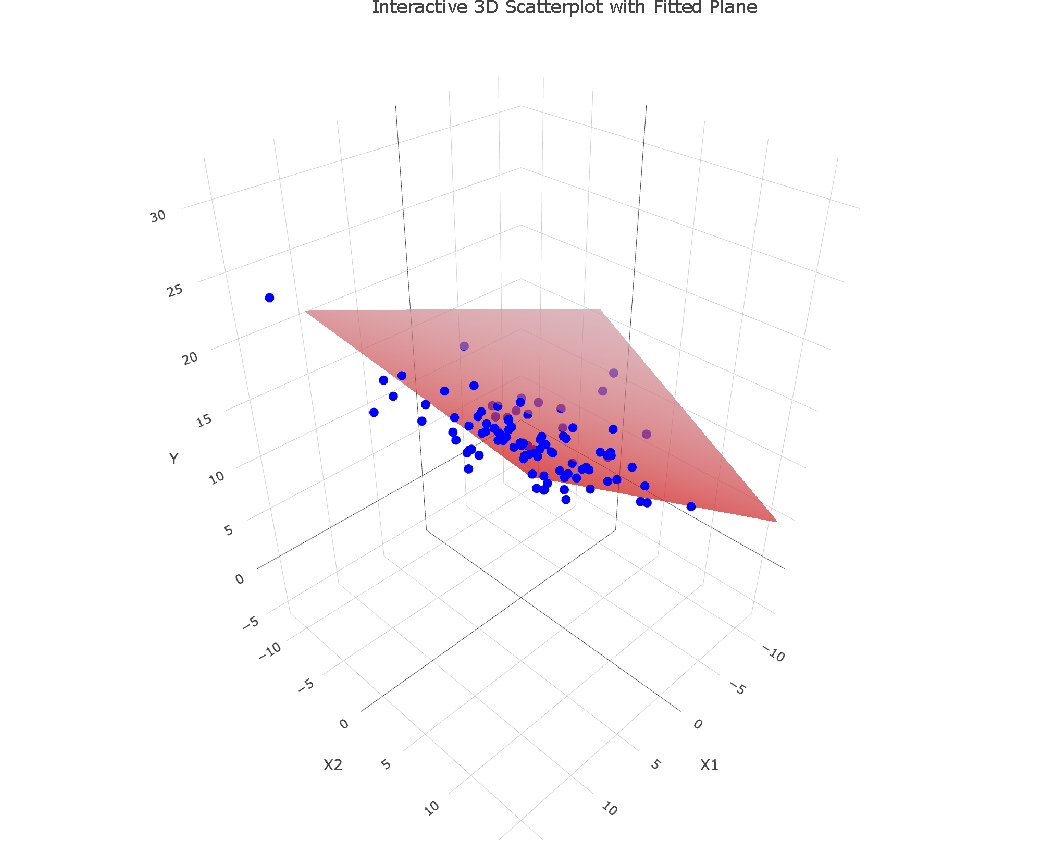
\includegraphics[keepaspectratio]{bookdown-demo_files/figure-latex/unnamed-chunk-66-1.pdf}}

The term \texttt{X1\ *\ X2} is a shortcut for \texttt{X1\ +\ X2\ +\ X1:X2} where \texttt{X1:X2} is the interaction term.
R automatically includes the main effects of the predictors when an interaction term is included.
The true but usually unknown \(\beta\)s are estimated quite precisely.

\subsubsection{Formal test for interaction}\label{formal-test-for-interaction}

We could apply a formal test for the interaction term by model comparison.
The command \texttt{anova(.,\ .)} would compare the two models and test if the change in the
residual sum of squares is statistically interesting.

\begin{Shaded}
\begin{Highlighting}[]
\NormalTok{m4}\FloatTok{.5} \OtherTok{\textless{}{-}} \FunctionTok{lm}\NormalTok{(Y }\SpecialCharTok{\textasciitilde{}}\NormalTok{ X1 }\SpecialCharTok{+}\NormalTok{ X2, }\AttributeTok{data =}\NormalTok{ d) }\CommentTok{\# without interaction}
\FunctionTok{anova}\NormalTok{(m4}\FloatTok{.5}\NormalTok{, m4}\FloatTok{.4}\NormalTok{)}
\end{Highlighting}
\end{Shaded}

\begin{verbatim}
## Analysis of Variance Table
## 
## Model 1: Y ~ X1 + X2
## Model 2: Y ~ X1 * X2
##   Res.Df   RSS Df Sum of Sq      F    Pr(>F)    
## 1     97 38468                                  
## 2     96  2151  1     36316 1620.6 < 2.2e-16 ***
## ---
## Signif. codes:  0 '***' 0.001 '**' 0.01 '*' 0.05 '.' 0.1 ' ' 1
\end{verbatim}

One can show that the following test statistic is F distributed under the null hypothesis:

\[ F = \frac{\left(RSS_{\text{Model 1}} - RSS_{\text{Model 2}}\right) / \left(df_{\text{Model 1}} - df_{\text{Model 2}}\right)}{RSS_{\text{Model 2}} / df_{\text{Model 2}}}\]

where \(RSS\) is the residual sum of squares,
\(df\) are the degrees of freedom of the residual sum of squares for both models.

The output of the \texttt{anova} command shows us the residual degress of freedom (\texttt{Res.Df})
of both models, the residual sum of squares errors of both models (\texttt{RSS}),
the sum of squared errors between model 1 and model 2 (\texttt{Sum\ of\ Sq}), the value of the
F-statistic and the \(p\)-value for the hypothesis, that the coefficient for
the interaction term is zero (\(\beta_3=0\)). Model 1 RSS has 97 degrees of freedom, since we have 100 data points
and 3 parameters to estimate (\(\beta_0, \beta_1, \beta_2\)). Model 2 has 96 degrees of freedom, since
we have 100 data points and 4 parameters to estimate (\(\beta_0, \beta_1, \beta_2, \beta_3\)).

Let's verify the value of the F statistic:

\begin{Shaded}
\begin{Highlighting}[]
\NormalTok{RSS\_model1 }\OtherTok{\textless{}{-}} \FunctionTok{sum}\NormalTok{(}\FunctionTok{residuals}\NormalTok{(m4}\FloatTok{.5}\NormalTok{)}\SpecialCharTok{\^{}}\DecValTok{2}\NormalTok{)}
\NormalTok{RSS\_model2 }\OtherTok{\textless{}{-}} \FunctionTok{sum}\NormalTok{(}\FunctionTok{residuals}\NormalTok{(m4}\FloatTok{.4}\NormalTok{)}\SpecialCharTok{\^{}}\DecValTok{2}\NormalTok{)}
\NormalTok{df\_model1 }\OtherTok{\textless{}{-}}\NormalTok{ n }\SpecialCharTok{{-}} \FunctionTok{length}\NormalTok{(}\FunctionTok{coef}\NormalTok{(m4}\FloatTok{.5}\NormalTok{))}
\NormalTok{df\_model2 }\OtherTok{\textless{}{-}}\NormalTok{ n }\SpecialCharTok{{-}} \FunctionTok{length}\NormalTok{(}\FunctionTok{coef}\NormalTok{(m4}\FloatTok{.4}\NormalTok{))}
\NormalTok{F }\OtherTok{\textless{}{-}}\NormalTok{ ((RSS\_model1 }\SpecialCharTok{{-}}\NormalTok{ RSS\_model2) }\SpecialCharTok{/}\NormalTok{ (df\_model1 }\SpecialCharTok{{-}}\NormalTok{ df\_model2)) }\SpecialCharTok{/}\NormalTok{ (RSS\_model2 }\SpecialCharTok{/}\NormalTok{ df\_model2)}
\NormalTok{F}
\end{Highlighting}
\end{Shaded}

\begin{verbatim}
## [1] 1620.606
\end{verbatim}

\begin{Shaded}
\begin{Highlighting}[]
\CommentTok{\# Sum of Sq}
\NormalTok{RSS\_model1 }\SpecialCharTok{{-}}\NormalTok{ RSS\_model2}
\end{Highlighting}
\end{Shaded}

\begin{verbatim}
## [1] 36316.28
\end{verbatim}

In the numerator of the F statistic, we have the change in the residual sum of squares
(from the small (model 1) model to the larger one (model 2), \texttt{Sum\ of\ Sq})
per additional parameter in the model (one additional parameter \(\beta_3\)).

In the denominator, we have the residual sum of squares per residual degree of freedom of
the larger model (model 2). Hence, in the numerator we have the information on how much
better we get with respect to the number of variables added, and in the denominator
we have information on how good the full model is with respect to its degrees of freedom.

The \(p\)-value is the probability of observing a value of the F statistic as extreme or more
extreme than the one we observed, given that the null hypothesis is true. Here,
the \(p\)-value is extremely small. So, statistically we would see an improvement in RSS
which is not explainable by chance alone.
But \textbf{let's be careful with \(p\)-values} and especially with fixed cutoff values for \(\alpha\),
which we will \textbf{never} use in this script.
Even for a rather small effect \(\beta_3\), we would reject the null hypothesis, if only the sample
size is large enough. Since a very small effect relative to \(\beta_1\) and \(\beta_2\) would
probably not be of practical interest, one should be careful with looking at \(p\)-values alone.
For instance, in Richard McElreath's book \href{https://xcelab.net/rm/statistical-rethinking/}{Statistical Rethinking},
there are no \(p\)-values at all. I like that.

If you again look at the comparison of the RSS between the two models, you would
immediately see that the model with the interaction term is better (at least with respect to this metric).
The difference is huge. We have already mentioned in the context of \(R^2\) not to overinterpret
such metric, because RSS is monotonically descreasing with number of variables added and reaches
zero when the number of variables equals the number of data points (see \hyperref[exercise3_multiple_regression]{exercise 3}).

\subsection{Using an interaction plot to see a potential interaction}\label{interaction_plot}

Chronologically before we include an interaction term in the model, we can use an interaction plot
to see if there is a potential interaction between the predictors.
We can just create a catorical predictor out of the continuous predictors.
We just categorize the predictors into quartiles and plot the means of the dependent variable (\(Y\)).
If the lines are parallel, there is no interaction. If the lines are not parallel,
there might be an interaction.

\begin{Shaded}
\begin{Highlighting}[]
\NormalTok{n }\OtherTok{\textless{}{-}} \DecValTok{100}
\NormalTok{X1 }\OtherTok{\textless{}{-}} \FunctionTok{rnorm}\NormalTok{(n, }\DecValTok{0}\NormalTok{, }\DecValTok{5}\NormalTok{)}
\NormalTok{X2 }\OtherTok{\textless{}{-}} \FunctionTok{rnorm}\NormalTok{(n, }\DecValTok{0}\NormalTok{, }\DecValTok{5}\NormalTok{)}
\NormalTok{Y }\OtherTok{\textless{}{-}} \DecValTok{10} \SpecialCharTok{+} \FloatTok{0.5} \SpecialCharTok{*}\NormalTok{ X1 }\SpecialCharTok{+} \DecValTok{1} \SpecialCharTok{*}\NormalTok{ X2 }\SpecialCharTok{+} \FloatTok{0.89} \SpecialCharTok{*}\NormalTok{ X1 }\SpecialCharTok{*}\NormalTok{ X2 }\SpecialCharTok{+} \FunctionTok{rnorm}\NormalTok{(n, }\DecValTok{0}\NormalTok{, }\DecValTok{5}\NormalTok{)}
\NormalTok{d }\OtherTok{\textless{}{-}} \FunctionTok{data.frame}\NormalTok{(}\AttributeTok{X1 =}\NormalTok{ X1, }\AttributeTok{X2 =}\NormalTok{ X2, }\AttributeTok{Y =}\NormalTok{ Y)}

\CommentTok{\# Create categorical variables based on quartiles}
\NormalTok{d}\SpecialCharTok{$}\NormalTok{X2\_cat }\OtherTok{\textless{}{-}} \FunctionTok{cut}\NormalTok{(d}\SpecialCharTok{$}\NormalTok{X2, }
                \AttributeTok{breaks =} \FunctionTok{quantile}\NormalTok{(d}\SpecialCharTok{$}\NormalTok{X2, }\AttributeTok{probs =} \FunctionTok{c}\NormalTok{(}\DecValTok{0}\NormalTok{, }\FloatTok{0.25}\NormalTok{, }\FloatTok{0.5}\NormalTok{, }\FloatTok{0.75}\NormalTok{, }\DecValTok{1}\NormalTok{), }\AttributeTok{na.rm =} \ConstantTok{TRUE}\NormalTok{), }
                \AttributeTok{include.lowest =} \ConstantTok{TRUE}\NormalTok{, }
                \AttributeTok{labels =} \FunctionTok{c}\NormalTok{(}\StringTok{"Q1"}\NormalTok{, }\StringTok{"Q2"}\NormalTok{, }\StringTok{"Q3"}\NormalTok{, }\StringTok{"Q4"}\NormalTok{))}

\NormalTok{d}\SpecialCharTok{$}\NormalTok{X1\_cat }\OtherTok{\textless{}{-}} \FunctionTok{cut}\NormalTok{(d}\SpecialCharTok{$}\NormalTok{X1, }
                \AttributeTok{breaks =} \FunctionTok{quantile}\NormalTok{(d}\SpecialCharTok{$}\NormalTok{X1, }\AttributeTok{probs =} \FunctionTok{c}\NormalTok{(}\DecValTok{0}\NormalTok{, }\FloatTok{0.25}\NormalTok{, }\FloatTok{0.5}\NormalTok{, }\FloatTok{0.75}\NormalTok{, }\DecValTok{1}\NormalTok{), }\AttributeTok{na.rm =} \ConstantTok{TRUE}\NormalTok{), }
                \AttributeTok{include.lowest =} \ConstantTok{TRUE}\NormalTok{, }
                \AttributeTok{labels =} \FunctionTok{c}\NormalTok{(}\StringTok{"Q1"}\NormalTok{, }\StringTok{"Q2"}\NormalTok{, }\StringTok{"Q3"}\NormalTok{, }\StringTok{"Q4"}\NormalTok{))}

\CommentTok{\# Create the interaction plot}
\FunctionTok{interaction.plot}\NormalTok{(d}\SpecialCharTok{$}\NormalTok{X2\_cat, d}\SpecialCharTok{$}\NormalTok{X1\_cat, d}\SpecialCharTok{$}\NormalTok{Y)}
\end{Highlighting}
\end{Shaded}

\pandocbounded{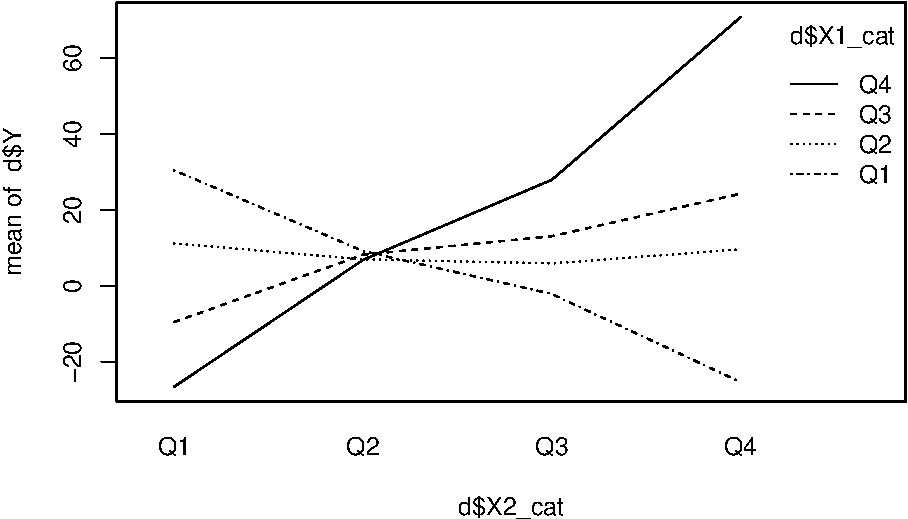
\includegraphics[keepaspectratio]{bookdown-demo_files/figure-latex/unnamed-chunk-69-1.pdf}}

There seems to be an intercation of the predictors with respect to \(Y\). The lines are not parallel.
If there was no interaction, the change in \(Y\) with respect to \(X_1\) would be the same for all levels of \(X_2\).
This seems not to be the case here.
See \hyperref[exercise5_multiple_regression]{exercise 5}.

If we had one or both predictors already categorical, we would not have to discretize them before.

\subsection{Simpsons Paradox}\label{simpsons-paradox}

The \href{https://en.wikipedia.org/wiki/Simpson\%27s_paradox}{Simpsons paradox} is a phenomenon,
in which a trend appears in several different groups of data but disappears
or reverses when these groups are combined. I agree with the criticism that this is not really
a paradox but a failure to consider confounding variables adequately. Let's quickly invent an example.
We are interested in the relationship hours of muscle training and strength (not based on evidence)
in children vs.~adults. Within both groups there will be an increasing relationship. The more training,
the more muscle strength. But if we combine the groups, we will see a decreasing relationship.

\begin{Shaded}
\begin{Highlighting}[]
\FunctionTok{library}\NormalTok{(tidyverse)}
\NormalTok{n }\OtherTok{\textless{}{-}} \DecValTok{100}
\NormalTok{age }\OtherTok{\textless{}{-}} \FunctionTok{c}\NormalTok{(}\FunctionTok{rep}\NormalTok{(}\StringTok{"child"}\NormalTok{, n}\SpecialCharTok{/}\DecValTok{2}\NormalTok{), }\FunctionTok{rep}\NormalTok{(}\StringTok{"adult"}\NormalTok{, n}\SpecialCharTok{/}\DecValTok{2}\NormalTok{))}
\NormalTok{training }\OtherTok{\textless{}{-}} \FunctionTok{c}\NormalTok{(}\FunctionTok{rnorm}\NormalTok{(n}\SpecialCharTok{/}\DecValTok{2}\NormalTok{, }\DecValTok{0}\NormalTok{, }\DecValTok{5}\NormalTok{) }\SpecialCharTok{+} \DecValTok{30}\NormalTok{, }\FunctionTok{rnorm}\NormalTok{(n}\SpecialCharTok{/}\DecValTok{2}\NormalTok{, }\DecValTok{0}\NormalTok{, }\DecValTok{5}\NormalTok{)}\SpecialCharTok{+} \DecValTok{10}\NormalTok{)}
\NormalTok{strength }\OtherTok{\textless{}{-}} \FunctionTok{c}\NormalTok{(}
  \DecValTok{10} \SpecialCharTok{+} \FloatTok{0.5} \SpecialCharTok{*}\NormalTok{ training[}\DecValTok{1}\SpecialCharTok{:}\NormalTok{(n}\SpecialCharTok{/}\DecValTok{2}\NormalTok{)] }\SpecialCharTok{+} \FunctionTok{rnorm}\NormalTok{(n}\SpecialCharTok{/}\DecValTok{2}\NormalTok{, }\DecValTok{0}\NormalTok{, }\DecValTok{2}\NormalTok{), }\CommentTok{\# For children}
  \DecValTok{25} \SpecialCharTok{+} \FloatTok{0.5} \SpecialCharTok{*}\NormalTok{ training[(n}\SpecialCharTok{/}\DecValTok{2} \SpecialCharTok{+} \DecValTok{1}\NormalTok{)}\SpecialCharTok{:}\NormalTok{n] }\SpecialCharTok{+} \FunctionTok{rnorm}\NormalTok{(n}\SpecialCharTok{/}\DecValTok{2}\NormalTok{, }\DecValTok{0}\NormalTok{, }\DecValTok{2}\NormalTok{) }\CommentTok{\# For adults}
\NormalTok{)}

\NormalTok{d }\OtherTok{\textless{}{-}} \FunctionTok{data.frame}\NormalTok{(}\AttributeTok{age =}\NormalTok{ age, }\AttributeTok{training =}\NormalTok{ training, }\AttributeTok{strength =}\NormalTok{ strength)}

\FunctionTok{ggplot}\NormalTok{(d, }\FunctionTok{aes}\NormalTok{(}\AttributeTok{x =}\NormalTok{ training, }\AttributeTok{y =}\NormalTok{ strength, }\AttributeTok{color =}\NormalTok{ age)) }\SpecialCharTok{+}
  \FunctionTok{geom\_point}\NormalTok{() }\SpecialCharTok{+}
  \FunctionTok{geom\_smooth}\NormalTok{(}\AttributeTok{method =} \StringTok{"lm"}\NormalTok{, }\AttributeTok{se =} \ConstantTok{FALSE}\NormalTok{) }\SpecialCharTok{+} \CommentTok{\# Group{-}specific regression lines}
  \FunctionTok{geom\_smooth}\NormalTok{(}\AttributeTok{data =}\NormalTok{ d, }\FunctionTok{aes}\NormalTok{(}\AttributeTok{x =}\NormalTok{ training, }\AttributeTok{y =}\NormalTok{ strength), }
              \AttributeTok{method =} \StringTok{"lm"}\NormalTok{, }\AttributeTok{se =} \ConstantTok{FALSE}\NormalTok{, }\AttributeTok{color =} \StringTok{"black"}\NormalTok{, }\AttributeTok{linetype =} \StringTok{"dashed"}\NormalTok{, }\AttributeTok{linewidth =} \FloatTok{1.2}\NormalTok{) }\SpecialCharTok{+} \CommentTok{\# Overall regression line}
  \FunctionTok{labs}\NormalTok{(}\AttributeTok{title =} \StringTok{"Regression Lines for Training and Strength"}\NormalTok{,}
       \AttributeTok{x =} \StringTok{"Training"}\NormalTok{,}
       \AttributeTok{y =} \StringTok{"Strength"}\NormalTok{) }\SpecialCharTok{+}
  \FunctionTok{theme\_minimal}\NormalTok{() }\SpecialCharTok{+} 
  \FunctionTok{theme}\NormalTok{(}\AttributeTok{plot.title =} \FunctionTok{element\_text}\NormalTok{(}\AttributeTok{hjust =} \FloatTok{0.5}\NormalTok{))}
\end{Highlighting}
\end{Shaded}

\begin{verbatim}
## `geom_smooth()` using formula = 'y ~ x'
## `geom_smooth()` using formula = 'y ~ x'
\end{verbatim}

\pandocbounded{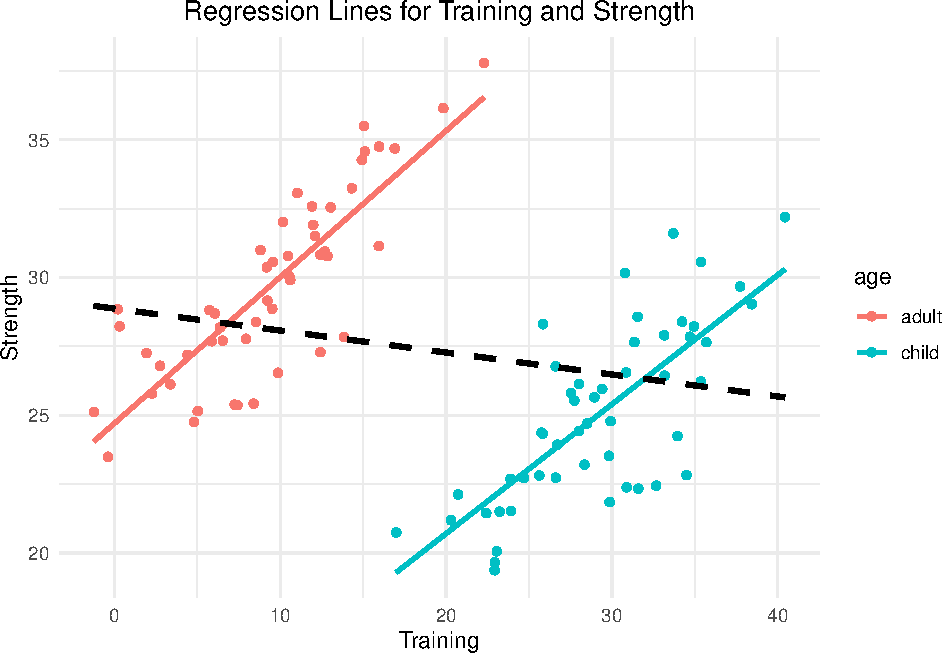
\includegraphics[keepaspectratio]{bookdown-demo_files/figure-latex/unnamed-chunk-70-1.pdf}}

\begin{itemize}
\tightlist
\item
  \textbf{Group-Specific Trends}:

  \begin{itemize}
  \tightlist
  \item
    In the group of \textbf{children} (blue line), strength \textbf{increases} with training, as indicated by the positive slope of the regression line.
  \item
    Similarly, in the group of \textbf{adults} (red line), strength also \textbf{increases} with training.
  \end{itemize}
\item
  \textbf{Overall Trend}:

  \begin{itemize}
  \tightlist
  \item
    When both groups are combined, the overall regression line (black, dashed) shows a \textbf{negative slope}, suggesting that \textbf{strength decreases} with training.
  \item
    This overall trend is opposite to the trends observed within the individual groups.
  \end{itemize}
\item
  \textbf{Why Does This Happen?}

  \begin{itemize}
  \tightlist
  \item
    This paradox occurs because the relationship between the grouping variable (\texttt{age}) and the independent variable (\texttt{training}) creates a confounding effect.
  \item
    In this case:

    \begin{itemize}
    \tightlist
    \item
      \textbf{Children} tend to have higher training values overall, while \textbf{adults} tend to have lower training values.
    \item
      The overall regression line reflects the imbalance between these groups rather than the true within-group relationships.
    \end{itemize}
  \end{itemize}
\end{itemize}

This (fictitious) example illustrates the importance of considering group-level differences when analyzing data.
In multiple regression this might not be so straightforward, since we cannot just plot the data and see the effect
as in our toy example. We will discuss this later.

Richard McElreath also has a nice example for this on \href{https://github.com/rmcelreath/causal_salad_2021/blob/main/1_causal_salad.r}{github}
and explains this in a \href{https://www.youtube.com/watch?v=KNPYUVmY3NM&ab_channel=RichardMcElreath}{video}.

\begin{Shaded}
\begin{Highlighting}[]
\FunctionTok{library}\NormalTok{(rethinking)}

\CommentTok{\# d{-}separation plots}
\NormalTok{a }\OtherTok{\textless{}{-}} \FloatTok{0.7}
\NormalTok{cols }\OtherTok{\textless{}{-}} \FunctionTok{c}\NormalTok{( }\FunctionTok{col.alpha}\NormalTok{(}\DecValTok{1}\NormalTok{,a) , }\FunctionTok{col.alpha}\NormalTok{(}\DecValTok{2}\NormalTok{,a) )}

\CommentTok{\# pipe}
\NormalTok{N }\OtherTok{\textless{}{-}} \DecValTok{1000}
\NormalTok{X }\OtherTok{\textless{}{-}} \FunctionTok{rnorm}\NormalTok{(N)}
\NormalTok{Z }\OtherTok{\textless{}{-}} \FunctionTok{rbern}\NormalTok{(N,}\FunctionTok{inv\_logit}\NormalTok{(X))}
\NormalTok{Y }\OtherTok{\textless{}{-}} \FunctionTok{rnorm}\NormalTok{(N,(}\DecValTok{2}\SpecialCharTok{*}\NormalTok{Z}\DecValTok{{-}1}\NormalTok{))}

\FunctionTok{plot}\NormalTok{( X , Y , }\AttributeTok{col=}\NormalTok{cols[Z}\SpecialCharTok{+}\DecValTok{1}\NormalTok{] , }\AttributeTok{pch=}\DecValTok{16}\NormalTok{ )}
\FunctionTok{abline}\NormalTok{(}\FunctionTok{lm}\NormalTok{(Y[Z}\SpecialCharTok{==}\DecValTok{1}\NormalTok{]}\SpecialCharTok{\textasciitilde{}}\NormalTok{X[Z}\SpecialCharTok{==}\DecValTok{1}\NormalTok{]),}\AttributeTok{col=}\DecValTok{2}\NormalTok{,}\AttributeTok{lwd=}\DecValTok{3}\NormalTok{)}
\FunctionTok{abline}\NormalTok{(}\FunctionTok{lm}\NormalTok{(Y[Z}\SpecialCharTok{==}\DecValTok{0}\NormalTok{]}\SpecialCharTok{\textasciitilde{}}\NormalTok{X[Z}\SpecialCharTok{==}\DecValTok{0}\NormalTok{]),}\AttributeTok{col=}\DecValTok{1}\NormalTok{,}\AttributeTok{lwd=}\DecValTok{3}\NormalTok{)}
\FunctionTok{abline}\NormalTok{(}\FunctionTok{lm}\NormalTok{(Y}\SpecialCharTok{\textasciitilde{}}\NormalTok{X),}\AttributeTok{lwd=}\DecValTok{3}\NormalTok{,}\AttributeTok{lty=}\DecValTok{3}\NormalTok{)}
\end{Highlighting}
\end{Shaded}

\pandocbounded{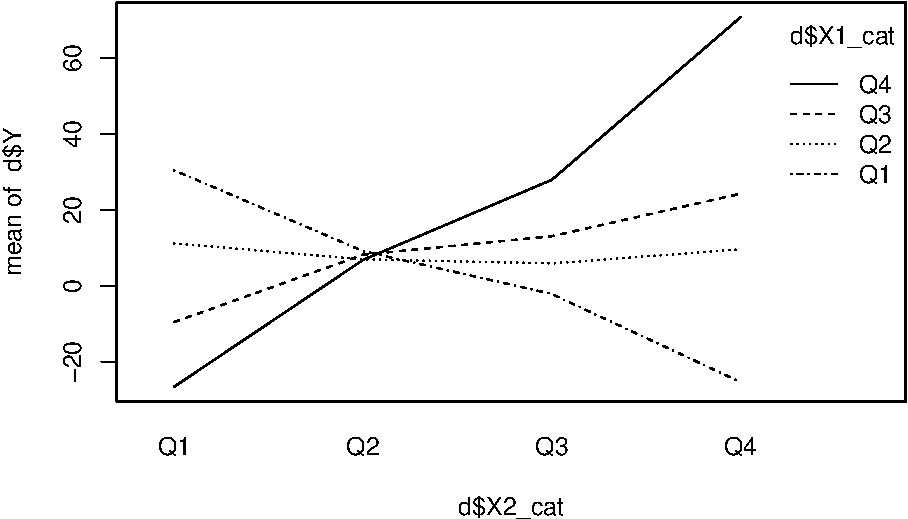
\includegraphics[keepaspectratio]{bookdown-demo_files/figure-latex/unnamed-chunk-71-1.pdf}}

\begin{Shaded}
\begin{Highlighting}[]
\CommentTok{\# fork}
\NormalTok{N }\OtherTok{\textless{}{-}} \DecValTok{1000}
\NormalTok{Z }\OtherTok{\textless{}{-}} \FunctionTok{rbern}\NormalTok{(N)}
\NormalTok{X }\OtherTok{\textless{}{-}} \FunctionTok{rnorm}\NormalTok{(N,}\DecValTok{2}\SpecialCharTok{*}\NormalTok{Z}\DecValTok{{-}1}\NormalTok{)}
\NormalTok{Y }\OtherTok{\textless{}{-}} \FunctionTok{rnorm}\NormalTok{(N,(}\DecValTok{2}\SpecialCharTok{*}\NormalTok{Z}\DecValTok{{-}1}\NormalTok{))}

\FunctionTok{plot}\NormalTok{( X , Y , }\AttributeTok{col=}\NormalTok{cols[Z}\SpecialCharTok{+}\DecValTok{1}\NormalTok{] , }\AttributeTok{pch=}\DecValTok{16}\NormalTok{ )}
\FunctionTok{abline}\NormalTok{(}\FunctionTok{lm}\NormalTok{(Y[Z}\SpecialCharTok{==}\DecValTok{1}\NormalTok{]}\SpecialCharTok{\textasciitilde{}}\NormalTok{X[Z}\SpecialCharTok{==}\DecValTok{1}\NormalTok{]),}\AttributeTok{col=}\DecValTok{2}\NormalTok{,}\AttributeTok{lwd=}\DecValTok{3}\NormalTok{)}
\FunctionTok{abline}\NormalTok{(}\FunctionTok{lm}\NormalTok{(Y[Z}\SpecialCharTok{==}\DecValTok{0}\NormalTok{]}\SpecialCharTok{\textasciitilde{}}\NormalTok{X[Z}\SpecialCharTok{==}\DecValTok{0}\NormalTok{]),}\AttributeTok{col=}\DecValTok{1}\NormalTok{,}\AttributeTok{lwd=}\DecValTok{3}\NormalTok{)}
\FunctionTok{abline}\NormalTok{(}\FunctionTok{lm}\NormalTok{(Y}\SpecialCharTok{\textasciitilde{}}\NormalTok{X),}\AttributeTok{lwd=}\DecValTok{3}\NormalTok{,}\AttributeTok{lty=}\DecValTok{3}\NormalTok{)}
\end{Highlighting}
\end{Shaded}

\pandocbounded{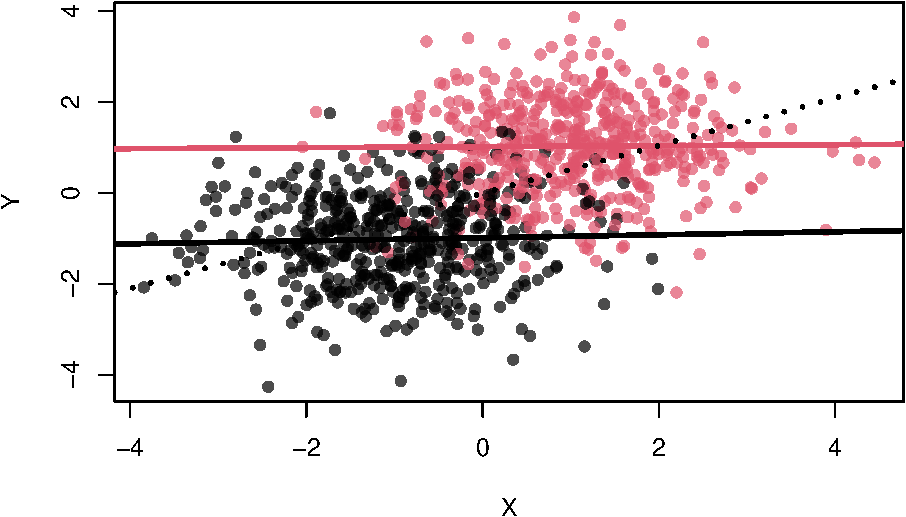
\includegraphics[keepaspectratio]{bookdown-demo_files/figure-latex/unnamed-chunk-71-2.pdf}}

\begin{Shaded}
\begin{Highlighting}[]
\CommentTok{\# collider}
\NormalTok{N }\OtherTok{\textless{}{-}} \DecValTok{1000}
\NormalTok{X }\OtherTok{\textless{}{-}} \FunctionTok{rnorm}\NormalTok{(N)}
\NormalTok{Y }\OtherTok{\textless{}{-}} \FunctionTok{rnorm}\NormalTok{(N)}
\NormalTok{Z }\OtherTok{\textless{}{-}} \FunctionTok{rbern}\NormalTok{(N,}\FunctionTok{inv\_logit}\NormalTok{(}\DecValTok{2}\SpecialCharTok{*}\NormalTok{X}\SpecialCharTok{+}\DecValTok{2}\SpecialCharTok{*}\NormalTok{Y}\DecValTok{{-}2}\NormalTok{))}

\FunctionTok{plot}\NormalTok{( X , Y , }\AttributeTok{col=}\NormalTok{cols[Z}\SpecialCharTok{+}\DecValTok{1}\NormalTok{] , }\AttributeTok{pch=}\DecValTok{16}\NormalTok{ )}
\FunctionTok{abline}\NormalTok{(}\FunctionTok{lm}\NormalTok{(Y[Z}\SpecialCharTok{==}\DecValTok{1}\NormalTok{]}\SpecialCharTok{\textasciitilde{}}\NormalTok{X[Z}\SpecialCharTok{==}\DecValTok{1}\NormalTok{]),}\AttributeTok{col=}\DecValTok{2}\NormalTok{,}\AttributeTok{lwd=}\DecValTok{3}\NormalTok{)}
\FunctionTok{abline}\NormalTok{(}\FunctionTok{lm}\NormalTok{(Y[Z}\SpecialCharTok{==}\DecValTok{0}\NormalTok{]}\SpecialCharTok{\textasciitilde{}}\NormalTok{X[Z}\SpecialCharTok{==}\DecValTok{0}\NormalTok{]),}\AttributeTok{col=}\DecValTok{1}\NormalTok{,}\AttributeTok{lwd=}\DecValTok{3}\NormalTok{)}
\FunctionTok{abline}\NormalTok{(}\FunctionTok{lm}\NormalTok{(Y}\SpecialCharTok{\textasciitilde{}}\NormalTok{X),}\AttributeTok{lwd=}\DecValTok{3}\NormalTok{,}\AttributeTok{lty=}\DecValTok{3}\NormalTok{)}
\end{Highlighting}
\end{Shaded}

\pandocbounded{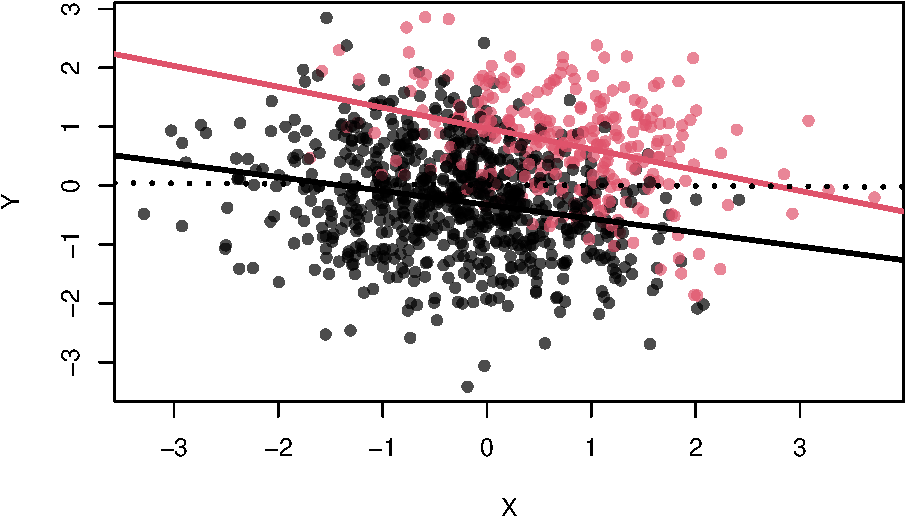
\includegraphics[keepaspectratio]{bookdown-demo_files/figure-latex/unnamed-chunk-71-3.pdf}}

\section{Exercises}\label{exercises-2}

\subsection{{[}M{]} Exercise 1}\label{exercise1_multiple_regression}

\begin{itemize}
\tightlist
\item
  Fit a model with a cubic term for weight and height of the !Kung San people.
\item
  Add the prediction bands as seen in the book.
\item
  Come up with an explanation for the functional form of this relationship.
\item
  Could there be reasons to for taking a less complicated model
  (\href{https://en.wikipedia.org/wiki/Statistical_model_specification}{1}, \href{https://en.wikipedia.org/wiki/Occam\%27s_razor}{2})?
\end{itemize}

\subsection{{[}E{]} Exercise 2}\label{exercise2_multiple_regression}

Consider the model equations from \hyperref[adding_transformed_predictor]{above}
where we used polynomial regression to model the relationship between
weight and height:

\begin{itemize}
\tightlist
\item
  Draw the model hierarchy for the model.
\end{itemize}

\subsection{{[}H{]} Exercise 3}\label{exercise3_multiple_regression}

Invent a data set (or use the first 3 lines of a previous data set)
with 3 observations of \(Y\) and \(X_1, X_2\) and \(X_3\). You have a data frame
with 3 rows and 4 columns.

\begin{itemize}
\tightlist
\item
  Fit a model with \(Y\) as the dependent variable and \(X_1, X_2, X_3\) as predictors.
\item
  How big is \(R^2\)?
\item
  Could you have calulated this without \texttt{lm}and R?
\end{itemize}

\subsection{{[}E{]} Exercise 4}\label{exercise4_multiple_regression}

Go back to the \hyperref[interaction_term]{section about the interaction term} in the linear model.

\begin{itemize}
\tightlist
\item
  Use the code provided
\item
  Standardise the predictors. How are the \(\beta\)s changing and what is their interpration now?
\item
  Change the relative sizes of the true but usually unknown \(\beta\)s.
  What happens to the estimates and the graph?
\item
  What happens if you change the error term and increase or decrease its variance?
\end{itemize}

\subsection{{[}E{]} Exercise 5}\label{exercise5_multiple_regression}

Draw the interaction plot from the \hyperref[interaction_plot]{section about the interaction plot}
for the case when there is not interaction, i.e.~\(\beta_3 = 0\).

\subsection{{[}M{]} Exercise 6}\label{exercise6_multiple_regression}

Go back to the model assumptions checks \hyperref[check_model_bayes]{above}.

\begin{itemize}
\tightlist
\item
  Create the same two plots for the simple mean model without predictors, just with the intercept.
\item
  Which model fits the data better according to these posterior predictive checks?
\end{itemize}

\section{TODOS}\label{todos}

\begin{itemize}
\tightlist
\item
  Add more Bayesian model checks, chapter 6 Gelman.
\item
  If you add a lot of variables to your regression model, you can get an arbitrarily large (\(\le 1\))
  \(R^2\). We will verify this when we have more than 2 explanatory variables.
\item
  maybe create animation of points wiggling to get a feeling for the variability
\item
  Show by simulation what Gelman talks about with significant p values. So I scan the data
  for significant p values and then simulate data with the same effect size and see how often
  I get significant p values. Especially the next effect would be probably smaller,
  especially, if one did p-hacking! Calculate a priori probability for replication (def?).
\item
  Variability of confidence interval borders (draw from X\ldots)
\item
  Logistic Regression
\item
  Chapter: Sample size calculations for logistic and multivariate regression, Proportions, ICCs, t.test
\item
  Chapter about ICCs, but maybe reduced
\item
  clearer difference between prediction and explanation. why do we need causal inference and
  why do we have to be careful when we throw predictors into a model, how sure can we be that
  the model does what we want it to do?
\item
  causal terror of richards book, fork, pipe, collider
\item
  Angenommen man hat ein masking eines Effekts und der Model fit ist aber gut (keine Voraussetzung verletzt),
  ist diese Situation möglich?
\item
  What about 2 interactions?
\item
  Which variables should I include in a model and why?
\item
  Emphasize individual prediction (if not already) - cant get below \(\sigma\) in prediction
\item
  Include information of Kahnemans book, Thinking fast and slow. Specifically, regression
  is better than intuition. Intuition only works in a valid environment, where patterns
  can be obeserved. In non-valid environments, the wrong patterns are learned. Furthermore,
  regression using some simple scores is better than expert intuition. Also Meehl is mentioned
  by Kahneman.
\item
  What to do if regression assumptions are violated?
\item
  What about a real life data set?
\item
  What about papers?
\item
  Simulate a cohort of Master thesis with small sample sizes and assume
  that there is a true but unknown effect.
\end{itemize}

\bibliography{book.bib,packages.bib}

\end{document}
